%%%%%%%%%%%%%%%%%%%%%%%%%%%%%%%%%%%%%%%%%
% Masters/Doctoral Thesis 
% LaTeX Template
% Version 2.5 (27/8/17)
%
% This template was downloaded from:
% http://www.LaTeXTemplates.com
%
% Version 2.x major modifications by:
% Vel (vel@latextemplates.com)
%
% This template is based on a template by:
% Steve Gunn (http://users.ecs.soton.ac.uk/srg/softwaretools/document/templates/)
% Sunil Patel (http://www.sunilpatel.co.uk/thesis-template/)
%
% Template license:
% CC BY-NC-SA 3.0 (http://creativecommons.org/licenses/by-nc-sa/3.0/)
%
%%%%%%%%%%%%%%%%%%%%%%%%%%%%%%%%%%%%%%%%%

%----------------------------------------------------------------------------------------
%	PACKAGES AND OTHER DOCUMENT CONFIGURATIONS
%----------------------------------------------------------------------------------------
\documentclass[
12pt, % The default document font size, options: 10pt, 11pt, 12pt
%oneside, % Two side (alternating margins) for binding by default, uncomment to switch to one side
english, % ngerman for German
onehalfspacing, % Single line spacing, alternatives: singlespacing or doublespacing
%draft, % Uncomment to enable draft mode (no pictures, no links, overfull hboxes indicated)
nolistspacing, % If the document is onehalfspacing or doublespacing, uncomment this to set spacing in lists to single
liststotoc, % Uncomment to add the list of figures/tables/etc to the table of contents
%toctotoc, % Uncomment to add the main table of contents to the table of contents
parskip, % Uncomment to add space between paragraphs
%nohyperref, % Uncomment to not load the hyperref package
headsepline, % Uncomment to get a line under the header
chapterinoneline, % Uncomment to place the chapter title next to the number on one line
% consistentlayout, % Uncomment to change the layout of the declaration, abstract and acknowledgements pages to match the default layout
]{MastersDoctoralThesis} % The class file specifying the document structure

% Font and language packages
\usepackage{polyglossia}
\setmainlanguage{english}
% \setotherlanguages{arabic}
\setotherlanguages{arabic, japanese, korean, thai, russian, ukrainian, greek} 

\usepackage{fontspec}
\newfontfamily\arabicfont[Script=Arabic]{Amiri}
\newfontfamily\japaneseFont{IPAMincho} % or any font that supports Kanji, Hiragana, and Katakana
\newcommand{\japaneseText}[1]{{\japaneseFont #1}}


\newfontfamily\koreanfont{NanumGothic} % Supports Hangul
\newfontfamily\thaifont{Norasi} % or any other font that supports Thai script
\newfontfamily\cyrillicfont{Times New Roman} % Just as an example; use a font that supports Cyrillic
\newfontfamily\greekfont{Times New Roman}


% Linking and PDF metadata
\usepackage{hyperref}

% Removed inputenc and fontenc as they are not required with LuaLaTeX/XeLaTeX
% \usepackage[utf8]{inputenc} % LuaLaTeX and XeLaTeX assume UTF-8 by default
% \usepackage[T1]{fontenc} % Not needed with LuaLaTeX/XeLaTeX

% Palatino font for text (optional)
\usepackage{mathpazo}

% Bibliography
\usepackage[backend=biber,style=authoryear,natbib=true]{biblatex}
\addbibresource{bibliography.bib}
\usepackage{pdfpages}
% Additional packages
\usepackage{todonotes}
\usepackage[autostyle=true]{csquotes} % For language-dependent quotes in the bibliography

% For adjusting figure sizes and rotations
\usepackage[export]{adjustbox}
\usepackage{rotating}

% For handling data tables
\usepackage{pgfplotstable}
\pgfplotsset{compat=1.18}

% Set the path to your images
\graphicspath{{images/}}

%----------------------------------------------------------------------------------------
%	MARGIN SETTINGS
%----------------------------------------------------------------------------------------

\geometry{
	paper=a4paper, % Change to letterpaper for US letter
	inner=2.5cm, % Inner margin
	outer=2.5cm, % Outer margin
	bindingoffset=.5cm, % Binding offset
	top=1.5cm, % Top margin
	bottom=1.5cm, % Bottom margin
	%showframe, % Uncomment to show how the type block is set on the page
}

%----------------------------------------------------------------------------------------
%	THESIS INFORMATION
%----------------------------------------------------------------------------------------
\thesistitle{Analyzing the Impact of Globalization on Color Naming Patterns Across Languages through Online Recruitment and Large Language Models}
% \thesistitle{Studying the Effect of Globalization on Color Perception using Multilingual Online Recruitment and Large Language Models} % Your thesis title, this is used in the title and abstract, print it elsewhere with \ttitle
\supervisor{Prof. Dr. Marc \textsc{Schönwiesner}} % Your supervisor's name, this is used in the title page, print it elsewhere with \supname
\examiner{Prof. Dr. Nori \textsc{Jacoby}} % Your examiner's name, this is not currently used anywhere in the template, print it elsewhere with \examname
\degree{M. Sc. Biology} % Your degree name, this is used in the title page and abstract, print it elsewhere with \degreename
\author{Jakob \textsc{Niedermann}} % Your name, this is used in the title page and abstract, print it elsewhere with \authorname
\addresses{} % Your address, this is not currently used anywhere in the template, print it elsewhere with \addressname

\subject{Biological Sciences} % Your subject area, this is not currently used anywhere in the template, print it elsewhere with \subjectname
\keywords{} % Keywords for your thesis, this is not currently used anywhere in the template, print it elsewhere with \keywordnames
\university{University Leipzig} % Your university's name and URL, this is used in the title page and abstract, print it elsewhere with \univname
\department{Fakultät für Lebenswissenschaften} % Your department's name and URL, this is used in the title page and abstract, print it elsewhere with \deptname
\group{AG Neurobiologie} % Your research group's name and URL, this is used in the title page, print it elsewhere with \groupname
\faculty{Faculty of Biology} % Your faculty's name and URL, this is used in the title page and abstract, print it elsewhere with \facname

\AtBeginDocument{
\hypersetup{pdftitle=\ttitle} % Set the PDF's title to your title
\hypersetup{pdfauthor=\authorname} % Set the PDF's author to your name
\hypersetup{pdfkeywords=\keywordnames} % Set the PDF's keywords to your keywords
}

\begin{document}

\frontmatter % Use roman page numbering style (i, ii, iii, iv...) for the pre-content pages

\pagestyle{plain} % Default to the plain heading style until the thesis style is called for the body content



%----------------------------------------------------------------------------------------
%	TITLE PAGE
%----------------------------------------------------------------------------------------

\begin{titlepage}
\begin{center}

\vspace*{.0\textheight}
{\scshape\LARGE \univname\par}\vspace{0cm} % University name
\textsc{\Large Master Thesis}\\[0.5cm] % Thesis type

\HRule \\[0.4cm] % Horizontal line
{\huge \bfseries \ttitle\par}\vspace{0.3cm} % Thesis title
\HRule \\[1.5cm] % Horizontal line
 
\begin{minipage}[t]{0.4\textwidth}
\begin{flushleft} \large
\emph{Author:}\\
{\authorname} % Author name - remove the \href bracket to remove the link
\end{flushleft}
\end{minipage}
\begin{minipage}[t]{0.4\textwidth}
\begin{flushright} \large
\emph{1. Gutachter:} \\
{\supname} \\ % Supervisor name - remove the \href bracket to remove the link
\vspace{5mm}
\emph{2. Gutachter:} \\
{\examname}
\end{flushright}
\end{minipage}\\[1cm]
 
% \vfill

\large \textit{A thesis submitted in fulfillment of the requirements\\ for the degree of \degreename}\\[0.3cm] % University requirement text
\textit{in the}\\[0.4cm]
\groupname\\\deptname\\[0cm] % Research group name and department name
 
% \vfill

{\large \today}\\[0cm] % Date
% 
\includegraphics{images/uni_leipzig_logo.png} % University/department logo - uncomment to place it
 
% \vfill
\end{center}
\end{titlepage}

%----------------------------------------------------------------------------------------
%	DECLARATION PAGE
%----------------------------------------------------------------------------------------

\begin{declaration}
\addchaptertocentry{\authorshipname} % Add the declaration to the table of contents
Hiermit erkläre ich, dass ich die vorliegende Arbeit selbständig verfasst habe und keine anderen als die angegebenen Quellen und Hilfsmittel benutzt habe. Alle Stellen der Arbeit, die wörtlich oder sinngemäß aus Veröffentlichungen oder aus anderweitigen Quellen entnommen wurden, sind als solche kenntlich gemacht. 

Diese Arbeit ist in gleicher oder ähnlicher Form noch bei keiner anderen Prüfungsbehörde eingereicht worden.

\vspace{5mm}
\noindent Unterschrift:\\
\rule[0.5em]{25em}{0.5pt} % This prints a line for the signaturehttps://www.overleaf.com/project/65af877d5c3a839be2c04913

 \vspace{5mm}
\noindent Ort, Datum:\\
\rule[0.5em]{25em}{0.5pt} % This prints a line to write the date
\end{declaration}

% \cleardoublepage

%----------------------------------------------------------------------------------------
%	QUOTATION PAGE
%----------------------------------------------------------------------------------------

%\vspace*{0.2\textheight}

%\noindent\enquote{\itshape Thanks to my solid academic training, today I can write hundreds of words on virtually any topic without possessing a shred of information, which is how I got a good job in journalism.}\bigbreak

%\hfill Dave Barry

%----------------------------------------------------------------------------------------
%	ABSTRACT PAGE
%----------------------------------------------------------------------------------------

\begin{abstract}
\addchaptertocentry{\abstractname} % Add the abstract to the table of contents
Is my blue your celeste? 
Although seeing the exact same physical colors, people of different languages use different terms to describe them. The influence of language and culture on perception is a longstanding problem in cognitive science and extensively studied e.g. in the World Color Survey. Berlin and Kay (1969) recruited participants speaking unwritten languages and asked them to describe a set of 330 Munsell color chips using color terms. They concluded that different languages use a subset or all of eleven "Basic" Color Terms. These categories are arranged according to strict evolutionary laws. Cross-lingual differences are hypothesized to decrease as a result of globalization, which explains the absence of a comprehensive and consistent data set for industrialized nations.

This research project employs Lucid as a new recruiter for online experiments with a massively expanded range of 112 targetable countries and 73 languages. A free elicitation naming paradigm was used to collect data from 4,351 participants in 25 languages. Analysis of the data showed preserved structural differences in the naming pattern of participants heavily exposed to globalization effects through the internet across languages, specifically the expected cross-cultural variation within the color category "blue".
Comparison to a dataset created using an analog procedure with GPT4 and GPT4-V as agents showed correlated naming pattern across languages. In addition, language specific differences are preserved in the responding behavior of GPT4. %However, GPT and GPT-4 agents use more color terms across languages compared with humans. 
The results show how diverse recruiting, as well as the use of machine learning, can help to revisit classical cognitive science questions.



\end{abstract}

%----------------------------------------------------------------------------------------
%	ACKNOWLEDGEMENTS
%----------------------------------------------------------------------------------------

\begin{acknowledgements}
\addchaptertocentry{\acknowledgementname} % Add the acknowledgements to the table of contents
I wish to express my profound gratitude to Prof. Dr. Nori Jacoby, who has been an invaluable supervisor and mentor throughout this project. His continuous guidance and expertise have been crucial to the research and writing process. His enthusiasm for research is infectious, and I am fortunate to have absorbed some of it.
I extend my thanks to Pol van Rijn for his mentorship in both the technical aspects and theoretical inspiration of this work. His willingness to dedicate so much time has significantly shaped the direction and quality of this thesis.
My appreciation also goes out to all members of Prof. Dr. Nori Jacoby's research group, whose inclusive and ambitious environment has been incredibly motivating.
I am grateful to my family, friends, and the 4,351 participants who took part in this study, each of whom has contributed immensely to this work.

The findings discussed in this dissertation have been submitted as a conference paper for CogSci and published as a preprint, available at: \url{https://osf.io/preprints/psyarxiv/3jvxw}, titled "Studying the Effect of Globalization on Color Perception using Multilingual Online Recruitment and Large Language Models."


\end{acknowledgements}

%----------------------------------------------------------------------------------------
%	LIST OF CONTENTS/FIGURES/TABLES PAGES
%----------------------------------------------------------------------------------------

\tableofcontents % Prints the main table of contents

\listoffigures % Prints the list of figures

\listoftables % Prints the list of tables

%----------------------------------------------------------------------------------------
%	ABBREVIATIONS
%----------------------------------------------------------------------------------------

\begin{abbreviations}{ll} % Include a list of abbreviations (a table of two columns)

\textbf{BCT} & Basic Color Terms\\
\textbf{ARI} & Adjusted Rand Index\\
\textbf{MDS} & Multidimensional Scaling\\
\textbf{WCS} & World Color Survey\\
\textbf{SD} & Standard Deviation\\
\textbf{LLM} & Large Language Model\\
\textbf{VLM} & Vision Language Models\\
\textbf{MTurk} & amazon mechanical turk\\

\end{abbreviations}

%----------------------------------------------------------------------------------------
%	PHYSICAL CONSTANTS/OTHER DEFINITIONS
%----------------------------------------------------------------------------------------

%\begin{constants}{lr@{${}={}$}l} % The list of physical constants is a three column table

% The \SI{}{} command is provided by the siunitx package, see its documentation for instructions on how to use it

%Speed of Light & $c_{0}$ & \SI{2.99792458e8}{\meter\per\second} (exact)\\
%Constant Name & $Symbol$ & $Constant Value$ with units\\

%\end{constants}

%----------------------------------------------------------------------------------------
%	SYMBOLS
%----------------------------------------------------------------------------------------

%\begin{symbols}{lll} % Include a list of Symbols (a three column table)

%$a$ & distance & \si{\meter} \\
%$P$ & power & \si{\watt} (\si{\joule\per\second}) \\
%Symbol & Name & Unit \\

%\addlinespace % Gap to separate the Roman symbols from the Greek

%$\omega$ & angular frequency & \si{\radian} \\

%\end{symbols}

%----------------------------------------------------------------------------------------
%	DEDICATION
%----------------------------------------------------------------------------------------

\dedicatory{} 

%----------------------------------------------------------------------------------------
%	THESIS CONTENT - CHAPTERS
%----------------------------------------------------------------------------------------

\mainmatter % Begin numeric (1,2,3...) page numbering

\pagestyle{thesis} % Return the page headers back to the "thesis" style

% Include the chapters of the thesis as separate files from the Chapters folder
% Uncomment the lines as you write the chapters


\chapter{Introduction}
\section{Introduction}

According to the Sapir-Whorf hypothesis, we perceive and interact with our environment through the filters and categories of our language. The ability to talk about situations or characteristics of objects alters the way we perceive them \parencite{blasi2022over,kramsch2014language, whorfLanguage2012}.
In the field of cognitive science, the way in which culture including economy \parencite{fine2016world,henrich2001search}, values \parencite{inglehart2000world,triandis2018individualism} and language influence cognition is an object of intense investigation \parencite{barrett2020towards, henrichWeirdest2010}. 
The domain of color terms is a classic case-study for investigating culture-perception interaction because it has a directly measurable physiological correspondence.
It has been empirically demonstrated that when presented with the same color patches, people speaking different languages use different naming patterns. 

In a seminal work, Berlin and Kay subdivided color space into 330 Munsell Chips (Fig. \ref{fig:mode_prop_maps} upper panel) and ask participants to name these colors using "basic" color terms \parencite{berlinBasic1969}.
In the World Color Survey (WCS) \parencite{kayWorld2009} they examined 110 unwritten languages spoken solely of small scale societies.
From the investigation of these data they derived two main findings: First, different languages use different naming patterns - especially concerning the number of color terms. They claimed to have found a set of maximally eleven basic color categories. Languages make use of these terms or a subset of them down to three color terms. 
Second, languages using the same number of color terms exhibit similarities in the position of these categories in color space. This suggests universal rules shaping color terminology across languages.

\textcite{berlinBasic1969} suggested that exposure to global cultural influences has a leveling effect on the linguistic differences towards the eleven Basic Color Terms (BCT) in English vocabulary.
This is also why there was no large-scale, standardized, contemporary color-naming data collection at a global scale for industrialized languages. 
For some languages data sets exist but these investigations mostly concentrate on single languages and therefore differ in methodology and availability (for example \cite{lindseyColor2014,al-rasheedFurther2014, daviesBasic1994, kurikiModern2017, ozgenTurkish1998, thierryUnconscious2009, zollingerWhy1984,winawerRussian2007,berlinBasic1969}).

Globalization is a process having a heavy impact on informational flux and cultural exchange around the globe \parencite{barrett2020towards, pieterse2019globalization}. The work of this thesis is dedicated to the investigation of globalization effects on perception, particularly in the area of color terms.

With the recent publication of Large Language Models (LLM) e.g. GPT4 \parencite{achiam2023gpt} trained on all texts available online, another question can be addressed. If color perception is influenced by language and therefore conserved within text, are LLMs capable of reproducing language specific color naming patterns?

LLMs such as GPT4 \parencite{achiam2023gpt}, which are trained on extensive text corpora, have opened up a new line of inquiry.
%With the increase use of LLMs such as GPT4 \parencite{achiam2023gpt}, which are trained on extensive corpora of text accessible online, a novel line of inquiry emerges.
Since color perception is modulated by linguistic frameworks, and therefore embedded within textual corpora, can LLMs replicate language-specific color naming patterns?
In addition, the utilization of GPT4, a multilingual model subjected to extensive global cultural influences, may be considered as a proxy for a control group in assessing the impacts of globalization.

%In order to do justice to these impulses, 
To test this we collected data from human participants being native speakers of 25 distinct languages. Participants were recruited via the platform Lucid \parencite{lucid2024} , which served as a recruitment channel offering a non-traditional and diverse participant pool compared to traditional providers such as Amazon Mechanical Turk and Prolific.
In parallel, an analog dataset was created using the same procedure but engaging multilingual state-of-the-art LLMs (here GPT4; \cite{achiam2023gpt}) and Vision Language Models (VLMs, here GPT4V) as agents.

This thesis starts with an introduction describing the visual sense in general, ranging from light over the eye as the visual organ to the neurophysiological implementation in the brain stem and the visual cortex.
Then, I discuss the context information about the history and current state of knowledge in the field of color term research.
\section{Vision}

As a result of the properties of light, the sense of sight can be considered a "distant sense", similar to audition. As opposed to the sense of touch, our eyes perceive emitted light from distant objects rather than being in direct contact with them.

\subsection{Physical basis of light}

Consistent with the idea of sensing at a distance, "perceived light" itself is defined in the International Lighting Vocabulary (ILV) curated by the International Commission on Illumination (CIE) under the number \#17-22-039 with these properties in mind:

'light:
(perceived light)

\begin{itemize}
 \item Characteristic of all sensations and perceptions that is specific to the visual system
 \item Light is normally, but not always, perceived as a result of the action of a light stimulus on the visual system.'
\end{itemize}

This definition clarifies the distinction between perceived light and an object omitting light. In addition it highlights the role of the visual system to define light. 
%Something that excites the visual sense is normally considered to be light. 
Interestingly, visual light is a sub-range of the electromagnetic wave spectrum which can vary across different species and is defined by the properties of the sensual cells. For humans, this ranges from 380 to 700 nm wavelength (Fig. \ref{fig:VisLight}). In evolutionary terms, this has multiple causes.
Firstly, the solar emission of electromagnetic radiation peaks in the range of visible light. Additionally, the atmosphere surrounding the earth is most transparent for this range of wavelengths while absorbing much of the ultraviolet radiation below 300 nm and also reduces the transmission of infrared light above 700 nm. 
A similar transmission behaviour is observed for water, the medium in which the evolution of the eye started \parencite{born2013principles}.
%At least in the sense that there is no special property of this span of wavelength that is special compared to the rest. 
Other species such as bees are capable of seeing parts of the ultraviolet spectrum \parencite{slineyWhat2016}.

\begin{figure}[htp]
 \centering
 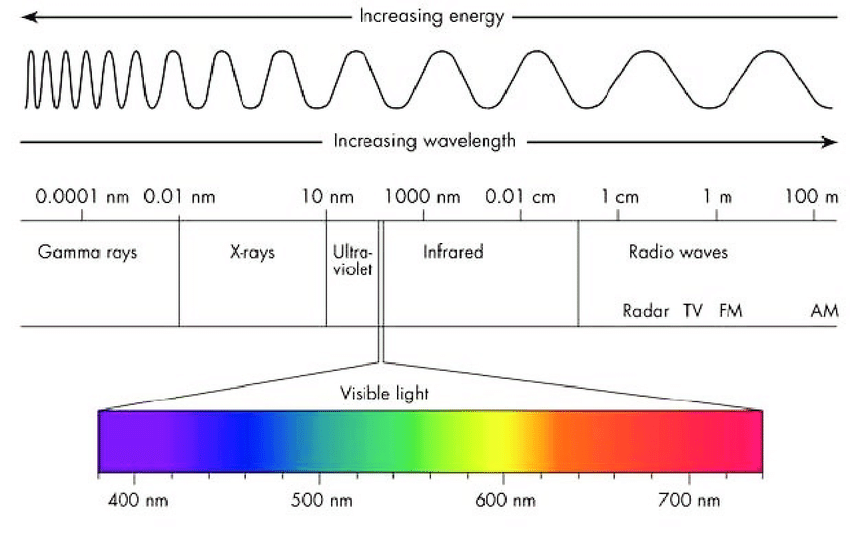
\includegraphics[width=\textwidth]{Diagram-of-the-lights-electromagnetic-spectrum-showing-the-different-wavelengths-of}
 \decoRule
 \caption[Spectrum of electromagnetic radiation]{Spectrum of electromagnetic radiation from large to small wavelengths (in nm) and, in more detail, the part of visual light from blue to red. Taken from \protect\textcite{SzantoiVisibleLightSpect}}
 \label{fig:VisLight}
\end{figure}

\subsection{Eye}

The sensory organ that processes light is the eye. The necessity for eyes has proven to be very urgent and apparently variable in evolution as it has developed up to 40 times independently by different metazoa \parencite{schwab2018evolution}.
%Ontogenetically, the human eye originates from both a protuberance of the neuroecto- (retina) and ectoderm (lens). 
The main structures of the eye that are responsible for perception are the lens and the retina. The lens focuses the incident light and ensures that the light can be collected more effectively. Variable shapes refract light differently, allowing objects at different distances to be focused. The incident light is then projected onto the opposite retina. The retina is a densely populated structure with, among other things, visually sensitive photo-receptor cells in which photo-transduction takes place, the conversion of light into a neuro-physiological receptor signal. A small area (ca. 0.2 mm diameter) of the retina directly opposite the lens is called the fovea. Here, the receptor cells are packed tight together, which enables extremely sharp vision \parencite{fatt2013physiology}.


\begin{figure}[htp]
 \centering
 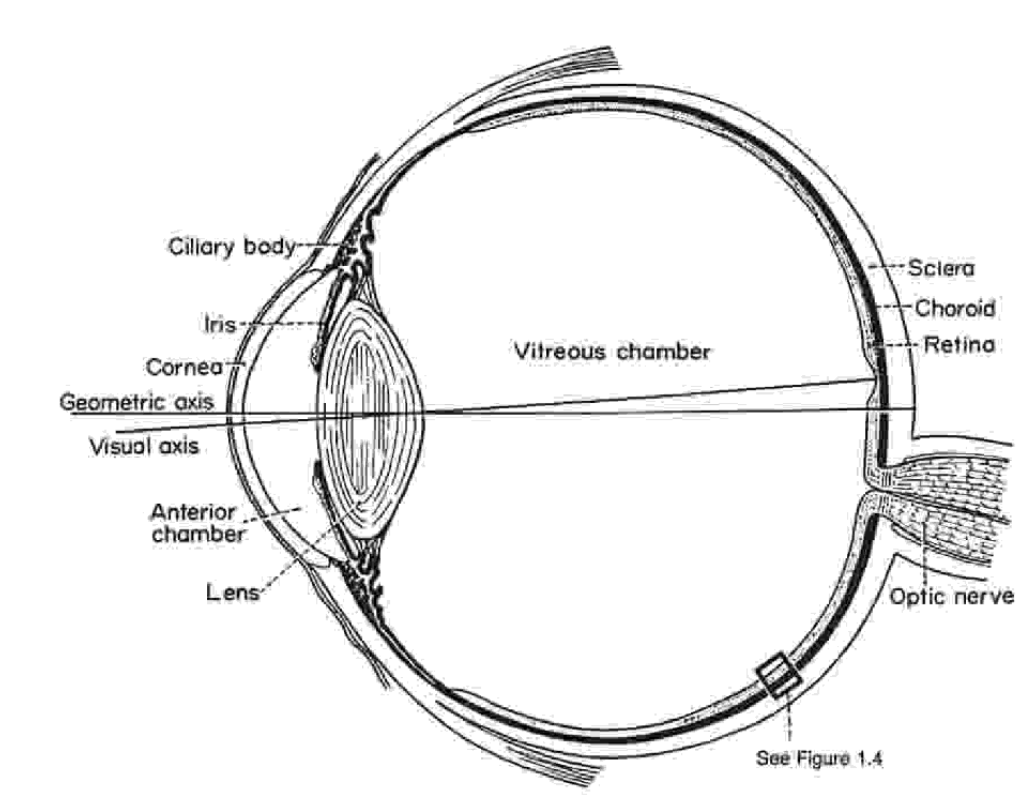
\includegraphics[width=\textwidth]{images/TheEye.png}
 \decoRule
 \caption[The Eye]{The Eye: Scientific drawing of the human eye, the organ responsible for the visual sense. Labels name the most important physiological structures, especially the lens that focuses light and the retina on which phototransduction takes place. Horizontal lines illustrate incident light rays hitting the retina. Taken from \protect\textcite{fatt2013physiology}}
 \label{fig:Eye}
\end{figure}

\subsection{Photo-receptors and Photo-transduction}
Photo-receptors consist of two parts. The inner segment is the cell body responsible for the general metabolism and the continuous construction of the outer segment. The outer segment is made up of membrane stacks which are permeated by Rhodopsin, a peptide composed of a trans-membrane domain and an attachment site for retinal. Retinal is a visual pigment that switches from 11-cis to all-trans configuration by the influence of a photon, thereby starting the phototransduction cascade, the initiation of the sensual process by creating a receptor potential. This signal is then transmitted via the synaptic terminal of the inner segment to the bipolar cells and then onto the ganglion cells. The axons of the bipolar cells form the optic nerve and therefore send signals to regions in the brain-stem \parencite{kolb1995webvision}. Importantly, the location of retinal cells is reflected in upstream areas, specifically in the optic nerve and later becomes prominent in the first visual cortex. This means that cells that are close together tend to send signals that are also processed in closely located areas in the upstream processing of the visual stimulations \parencite{selhorst2009optic}.


There are two types of photoreceptors that diverge in their shape and photoreception: Rods are thin, long and rod-shaped cells. They all contain the same visual pigment, which absorbs a wide range of wavelengths. Therefore, they are very efficient in collecting light, but they cannot distinguish between wavelengths. The perceptual outcome is black and white vision also in situations with low light exposure \parencite{kolb1995webvision}.

The cones are shorter and more cone-shaped. The outer segment does not contain as many membrane piles as rods. Thus, more light is necessary to elicit excitation of these cells. Cones are subdivided into three different types depending on the wavelength at which they maximally absorb. Short cones (S) absorb most efficiently short wavelengths which represents mostly blue and violet. Medium cones (M) absorb best in the green area, and long cones (L) are most sensitive to long wavelengths perceived as red. "S" cones are proportionally low in abundance, as the "M" and "L" cones occur around 100 times more often. But the overall relative composition of the different types is highly individual and might be the source of variation in color perception across humans. Namely, the brain uses the discrimination between wavelengths and the proportional excitation of these three types of receptor cells to process color vision \parencite{kolb1995webvision}.

In addition to the shape, cones and rods differ also in the region they occupy on the retina. The Fovea is almost exclusively populated with cones, while rods are placed in the periphery. Therefore, the Fovea is the place of color and the most precise vision. Low precision and non-chromatic vision of the peripheral regions are compensated for by constant scanning movements of the eye over the scenery and the brain's processing power, completing the mental image \parencite{kolb1995webvision}.


\subsection{Brain-stem}
The optical nerve leaving the eye is connected to the central nervous system. As a first step, the tracts cross in the Optic-Chiasm and through partial decussation information of both eyes coming from the right facial field is directed to the right hemisphere and vice versa. A smaller part of the nerve projects into the pretectal area, which is responsible for unconscious reflexes such as accommodation and pupillary reflex. Another subprojection aims for the superior colliculus which integrates somatosensory, auditory, and visual information in different layers forming, e.g. maps of the respective space. In "earlier" vertebrates this is the region of most complex processing and enables reflexes such as the intuitive focusing of newly approaching auditory or visual stimuli in the periphery. Furthermore, premotor areas code for movements towards specific areas in space. However, this region also integrates top down projections from the cortex which enables conscious intervention \parencite{fernandez2010anatomy, hubel1979BrainMech}.

The major part of the optical axons enter the Thalamus, more specifically, the corpus geniculatum laterale, which is considered to be the gatekeeper for all information entering the cortex and is constructed of six layers. These layers receive information from either the contra-lateral or ipsi-lateral side and are differentiated based on the ganglion cells from which they receive information. Layers one and two receive information from magnocellular ganglion cells, whereas layers 3 to 6 receive input from parvocellular ganglion cells. Magnocellular cells integrate over a broader number of sensory cells enabling the brain to process with higher speed and, therefore, support the perception of moving object in the visual scene. This is even exacerbated by heavily myelinated axons. The parvocellular ganglion cells integrate on fewer sensory cells, allowing for higher resolution and color perception \parencite{fernandez2010anatomy, hubel1979BrainMech}.

This differentiation represents the beginning of two hypothesized paths of visual processing that are supposed to be different in their objective: the "What" path and the "Where" path. The "What" path includes the precise identification of objects and their properties such as color or shape \parencite{grill2001lateral}. The "Where" path processes the rapid location of objects in space and their movement \parencite{gottlieb2007thought}. This separation is conserved in further processes in the cortex \parencite{ferrera1994responses, malach2002topography,mishkin1983object}.

\begin{figure}[htp]
 \centering
 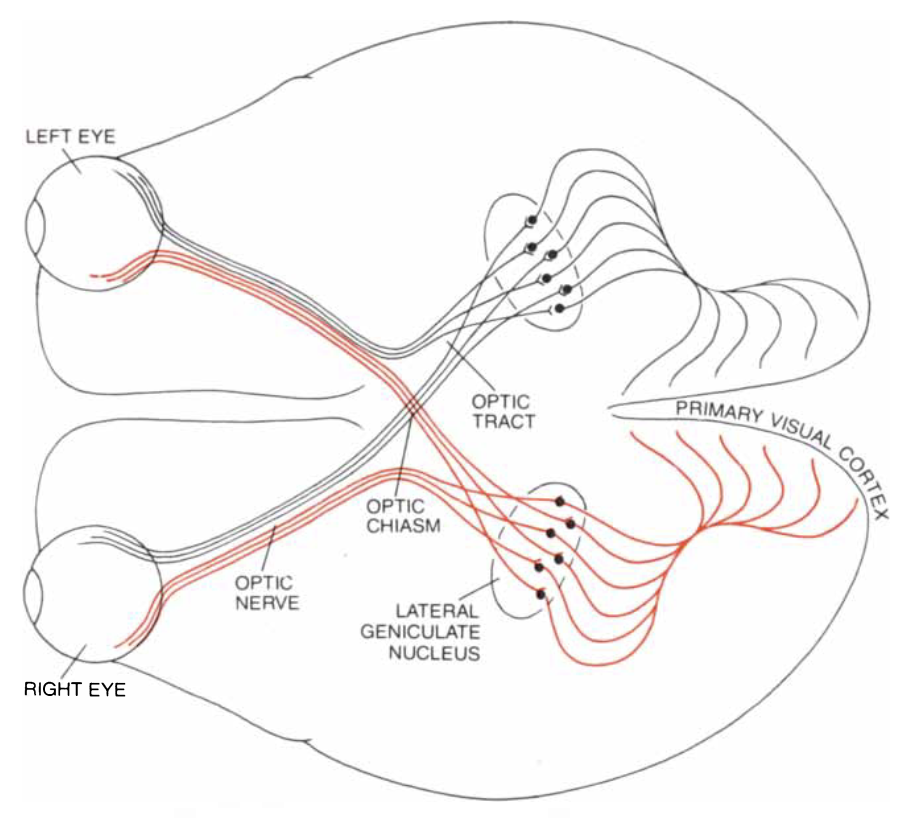
\includegraphics[width=\textwidth]{images/visual_pathway.png}
 \decoRule
 \caption[Visual Pathway]{Visual Pathway: The axons of the ganglion cells leave the retina and partially cross in the optic chiasm. Projections enter regions in the brain stem (pretectal area, Superior Colliculus, and the six layers of the lateral geniculate nucleus - thalamus). From there information is passed on to the primary visual cortex located in the occipital lobe.
 Taken from \protect\textcite{hubel1979BrainMech}}
 \label{fig:visual_pathway}
\end{figure}

\subsection{Visual Cortex}
Subsequently, the information is passed on to the fourth layer of the primary visual cortex, which is located in the occipital lobe. In the primary visual cortex, the retinotopic arrangement is conserved, which means that neighboring ganglion cells of the retina project to neighboring cells in the visual cortex. The overall organization is based on an the "ice-cube-model" \parencite{hubel1962receptive, hubel1979BrainMech}. Every point in the visual scene is represented by columns of neurons that respond to specific orientations of lines and edges. Additionally, there are so called blobs of neurons processing colors of the respective point in space \parencite{horton1984cytochrome, hubel1979BrainMech}. This implies that contours and colors in the visual scene are processed separately up until the second visual cortex. Once information leaves the visual cortex, it interacts with all other brain systems including memory, decision making and other executive functions \parencite{froudarakis2019Annual}. Ultimately, visual information contributes to actions. This hierarchy of processing is also a simplification. Naturally, sometime low level visual information is tightly integrated with actions and decision making. A simple example is a basketball player that needs to decide how to through a ball, coordinate visual information with its own motion and motor planning \parencite{pennartz2023howvisu}. 


From there, information is transmitted toward higher-order regions of the visual system. In the cortex visual processing is organized in different regions that are responsible for specific tasks of growing complexity, with "earlier" regions taking on more primitive tasks and higher-order areas such as the Inferior Temporal Lobe being engaged in complex tasks such as face recognition \parencite{sugase2011role}. The two previously mentioned paths can also be found here and determine the functions of the neighboring regions. Areas where an object's properties are studied are lined up around the temporal side of the cortex whereas regions that process motion are positioned toward the Paritetal Cortex \parencite{gegenfurtner1996interaction, niebur1995control}.


%\subsection{Higher order cortices and pathways}



% %! Author = jakobnieder
%! Date = 07.02.24


\section{Color term background}
\label{sec:Color_term_background}

\textcite{berlinBasic1969} collected color naming data on 320 chromatic and nine non-chromatic Munsell chips (\textcite{lennebergLanguage1956}; see Figure \ref{fig:munsell-chips}) from speakers of 20 languages in the Bay Area. Most of these speakers were bilingual. In a follow-up project, the ``World Color Survey" (WCS), linguists and anthropologists from around the world studied color naming patterns in 110 unwritten languages, many of them in small societies (Fig \ref{fig:wcs-locations}).

\begin{figure}[htbp]
\centering
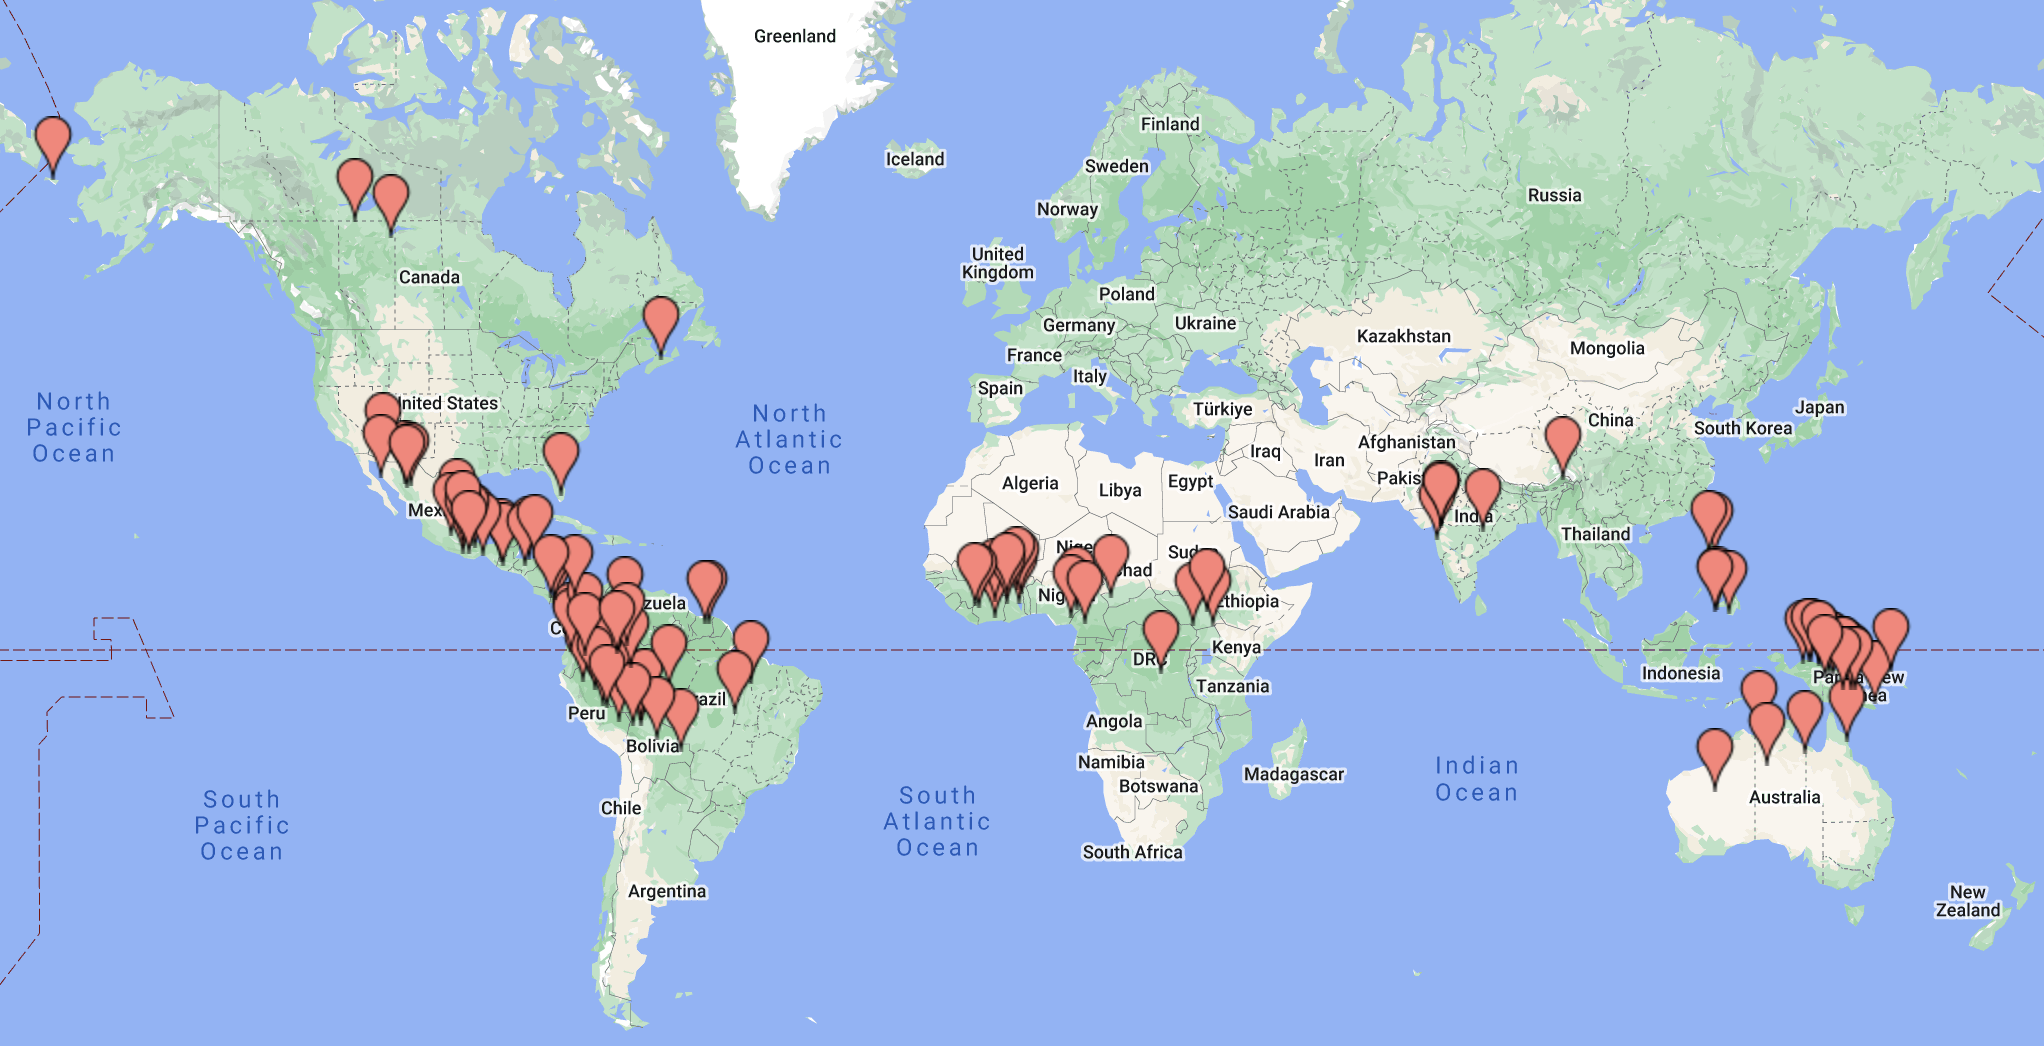
\includegraphics[width=\linewidth]{images/wcs-locations.png}
\decoRule
\caption[WCS Locations]{World map with information on the location of the 110 languages examined in the WCS.}
\label{fig:wcs-locations}
\end{figure}

Here, they used 330 Munsell chips, including 329 Munsell chips from the earlier study, plus one white chip. Their method included two stages. First, in a free naming task, participants named each chip in a fixed randomized order. In a second task (``focus task"), participants were asked to point to the color chip that best represents each unique color term used in the first task. This study concluded that having ``basic colors" -- a small set of commonly used color terms -- is universal. 

The systems of color terms themselves, however, varied greatly across languages. Nevertheless, they showed that languages with similar numbers of BCT tend to have similar mappings of terms to colors. Based on this, Berlin and Kay suggested that color terms systems develop from the simplest two color terms systems to more complex color systems with up to eleven color terms (\textit{black, white, red, yellow, green, blue, brown, orange, pink, purple, and gray})\parencite{berlinBasic1969,kayWorld2016}. According to this hypothesis, languages with similar numbers of terms have similar color maps because they went through the same constrained historical development trajectory. They received support by an approach by \textcite{lindseyUniversality2006} using k-means clustering, taking the naming pattern of each WCS participants as input. This analysis revealed successively forking categories from two to ten. The step wise results resembled with exceptions very well the actual categories present in the examined WCS languages and english. In addition, they identified regions of low concordance dividing roughly warm and cold colors across participants in color space. Both findings indicate consistent tendencies across languages dependent on the number of color terms.
\parencite{lindseyUniversality2006}

Across all WCS languages, \textcite{lindsey2009World} were able to categorize individual differences into six motives, reflecting the use of different subsets of BCT. The presence of two motives was replicated for English \parencite{lindseyColor2014}.

\begin{figure}[htbp]
\centering
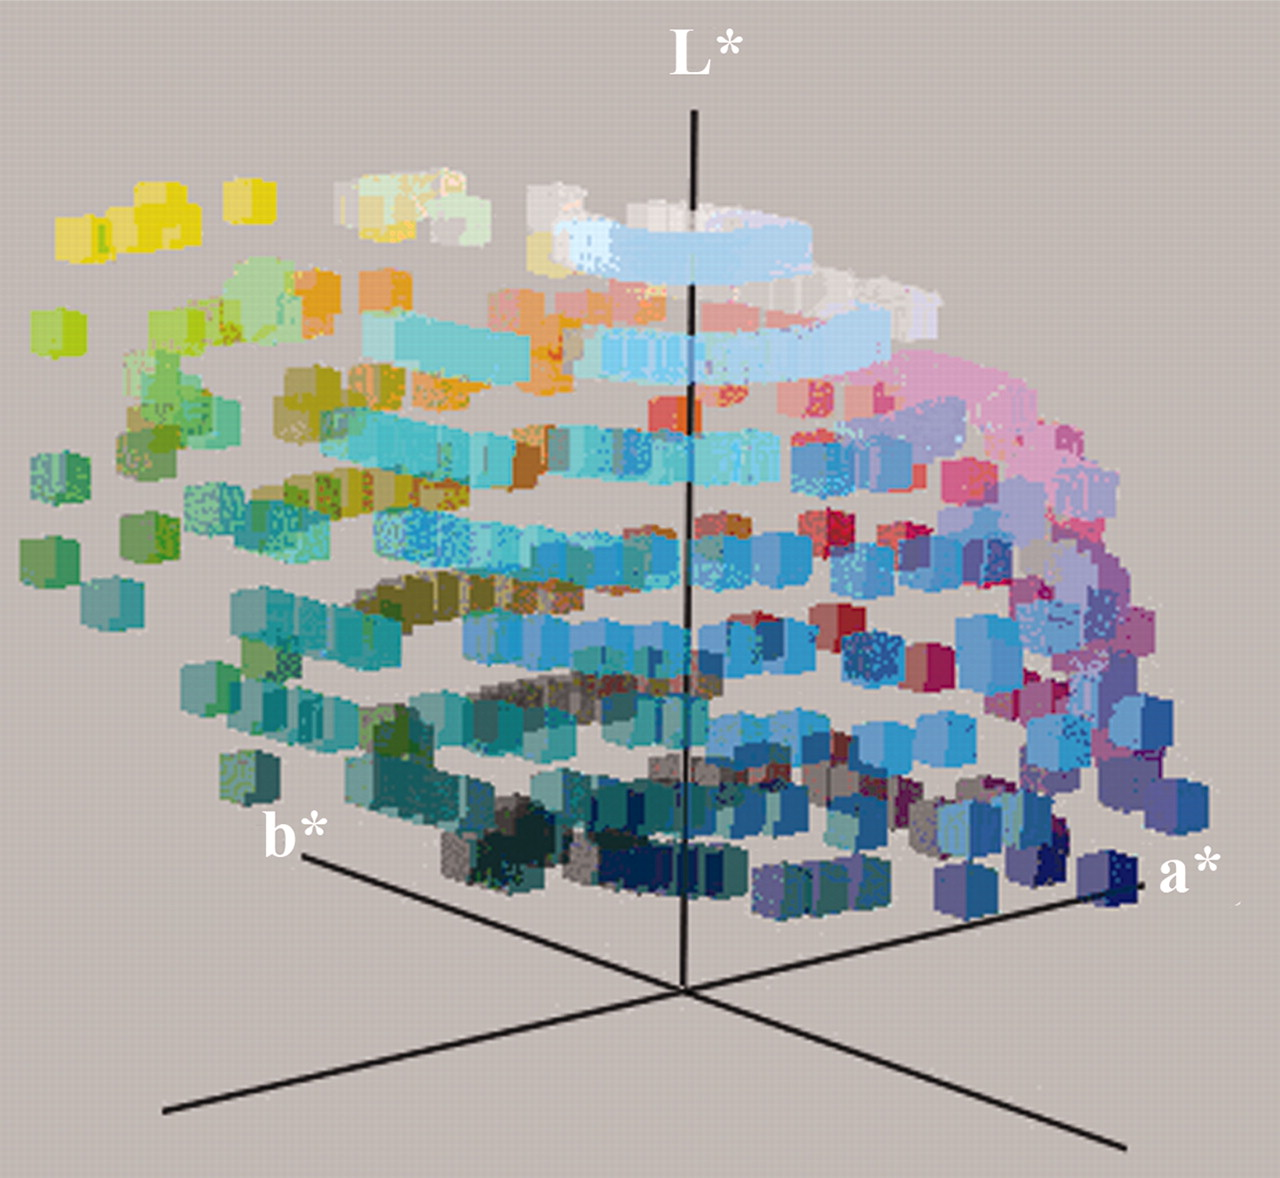
\includegraphics[width=\linewidth]{images/Cielab-space.jpeg}
\decoRule
\caption[Munsell Chips in Cielab Color Space.]{Munsell Chips in Cielab Color Space: 330 Musell color chips projected into Cielab color space. The irregular arrangement of the color chips is most prominent in the yellow region. \textcite{regierColor2007} used this irregularities and principles of categorization to explain the location and shape of color categories.
Taken from \textcite{regierColor2007}.}
\label{fig:Cielab_space}
\end{figure}

Subsequent theoretical work provided an alternative interpretation of the WCS findings. According to \textcite{regierColor2007}, the results of the WCS can be explained from two principles: a) a universally shared visual system, and b) an ``efficient'' organization of the lexicon. These universalist claims were pushed forward by an approach to predict color categories based on the mere irregularity of color space and basic assumptions of categorization. When converting the 330 color chips into the CIElab space, which constitutes a better psychophysical representation of the color space, the resulting locations of these color values do not yield a perfect symmetric shape (Fig. \ref{fig:Cielab_space}). 
A model using euclidean distances between color chips and rules of categorization to minimize similarity across categories and vice versa was able to predict naming patterns of real WCS languages. The model used a well formedness factor calculated as the sum of all distances of all chips of the same category and the distances of all chips that do not belong to the same category. When rotating the naming pattern along the L*axis, meaning to change the region of categories in the CIElab color space, the "Well-Formdness"-factor declined.
This was also true for languages that did not match the predictions of the model. Overall, these results support the hypothesis that color categories fit into optimal regions arranged by the universal peculiarities of color space \parencite{regierColor2007}.

% Change and add things
This idea was further developed by \textcite{zaslavskyEfficient2018}, proposing a unified formalization of “efficiency” using information theory. According to \textcite{zaslavskyEfficient2018}, efficient communication between speakers is characterized by an optimal trade-off between the complexity of the lexicon (as measured by the number of color terms) and the accuracy of communication. Therefore, languages with similar complexity have similar color maps because they provide similar optimal solutions to the problem of maximizing accuracy given a particular complexity.
The results of an iterated learning experiment performed by \textcite{xuCultural2013} are consistent with this communicative account. In the experiment, English-speaking participants were initially exposed to random assignments of color chips. The participants then generalized their responses to unseen chips after receiving some examples. The result of one participant was given to another participant, imitating cultural transmission in the real world. The systems of color terms produced by this process reproduced the structure of systems of color terms documented in the WCS.


Despite the impact of the World Color Survey, the data in the survey are limited to unwritten languages, mostly from small-scale societies and nonindustrial countries. Languages with many speakers, such as English, Spanish, French, and Portuguese, are missing from the survey. Part of the motivation for this omission was a concern that systems of color terms in industrial societies may have converged to similar structures as a result of contact through globalization. Data for these languages exist in the literature but are scattered in different papers with variations in methodology (for example, \textcite{forbesStructural1976, josserand:hal-03900005, lindseyColor2014, xuComparison2023}).


Several follow-up studies have further tested the findings of the WCS in a number of other languages and complementary paradigms. Most of these studies involved a small number of languages (e.g., German: \textcite{zollingerWhy1984}; Greek: \textcite{thierryUnconscious2009}; Turkish: \textcite{ozgenTurkish1998}). For example,\textcite{lindseyColor2014} asked participants to name colors in two different tasks. In the ``free elicitation task'', participants were asked to name colors freely using BCT, whereas, in the ``constrained naming task'', they had to use the eleven BCT elicited by \textcite{berlinBasic1969}.
Both groups showed fairly similar results with respect to the most frequently used color terms per color chip.

It is also well documented that some languages have greater diversity in terms of their shades of blue, in particular, Russian, Hebrew, and Italian \parencite{winawerRussian2007, CerquegliniHebrew, Paggetti2016ColorNI}. \textcite{winawerRussian2007} showed that Russian and English speakers differ not only in their color terminology, but also in the speed and accuracy of their discrimination of colors that fall into different color categories in one language and not the other.
% Several other languages also have a similar distinction between light and dark blue. For example,


% Color Term Evolution
Regarding Berlin and Kay's evolution hypothesis, follow-up studies declared to have found additional BCT for Russian \parencite{daviesBasic1994}, Greek \parencite{thierryUnconscious2009}, Turkish \parencite{ozgenTurkish1998} and German\parencite{zollingerWhy1984}. Another study by Lindsey and Brown proposed the stabilization of new color terms in English \parencite{lindseyColor2014}. This process of forming color categories is underpinned by a dual mechanism: it involves both the emergence between \parencite{levinsonYeli2000} and the partitioning \parencite{kayLinguistic1978} of preexisting color categories.
\parencite{lindseyColor2014}.
%They show, we can not be sure that previous datasets are not outdated by now.

Collecting new data could be specifically interesting to further deciphering these mechanisms of color term development especially for language where dataset already exist. Interestingly, several studies showed evidence for changes in the number of color terms within periods of just a few decades. For Japanese, for example, \textcite{kurikiModern2017} have reported that a large number of color categories have evolved significantly in less than fifty years. In another paper, \textcite{gibsonColor2017} documented changes in the number of color terms produced by Tsimane participants in the Bolivian Amazon and attributed these changes to industrialization due to the increased use of diversely colored artificial objects. In a large picture corpus investigation they discovered that objects are more likely to be colored in warm colors compared to the background. Subsequently, individuals exhibit increased precision and succinctness in naming warm color hues compared to their ability to articulate cold colors. Based on these observations, the researchers posited that the prevalent frequency of color usage acts as a catalyst, prompting the delineation and subsequent categorization of distinct chromatic nuances. In addition, they where able to show that Tsimane participants showed higher usage of color adjectives when describing artificial objects compared to natural objects. Thus, industrialization might drive the creation of new color categories simply by a greater use of diverse colored artificial objects.

\paragraph{\textbf{Color terms}}
The definition of BCT (BCT) is non trivial. The study of basic color term has long history (xxxxxxxx) but it was strongly promoted by aforementioned work by Berlin And Key \parencite{berlinBasic1969}.In this dissertation we operationally the definition to be commonly used in everyday life and not a compound word but a single word. Across the literature different explanations are given and different components are emphasized although this is a key factor to elicit comparable results \parencite{kayWorld2009 ,lindseyColor2014}. In fact, finding a definition that can be validly generalized across languages is a complex task. Some languages investigated during the WCS did not even have a word for color. In these cases experimenters were asked to use phrases like "How does it strike you eyes" \parencite{kayWorld2016}. In addition, the role and concept of compound words vary strongly across languages and make this definition less explicit. 
%In the case of Vietnamese it is not conclusively evident whether parts of a single word can be seperated by an "-" or if this already indicated that it is a compound word.


Another issue in the literature is the relationship between color terms and color categories. Often these two concepts are used interchangeably or mixed. However, this may poses problems, particularly when inferences are made from color terms and their use on color categories. \textcite{lindsey2009World} for example applied a k-means clustering algorithm on each individual naming pattern to identify a reasonable distribution of color categories independent of the actual term assigned. These categories are then named by the most common color term for this category. Even if they justify the level of this threshold the value remains arbitrary and distinct terms might be unified in single color categories. Therefore in the domain of color terms, clustering terms together is a strong unstable assumption. To avoid this loss of information, I propose alternative approach in this dissertation that does not commit to one category for each color. 
% Confusion of Color Categories and Terms
% A weakness in the studies mentioned so far is the confusion of color terms and categories.
% For the sake of clustering synonyms into one category the authors used k-means clustering to detect categories.
% However, we understand that in the domain of color terms, clustering terms together is a strong unstable assumption.
% Where to put the threshold to distinguish between two clusters?
% Especially in this research investigating the influence of language on perception we should stick to the actual color terms.
% Therefore, we propose that each color term should be treated as an own category.
% Hence, we strongly depend our analysis on color terms instead of clustered categories.


\section{Color term background}
\label{sec:Color_term_background2}


Naming different colors and therefore subdividing color space into discrete categories is an intuitive process.
However, it is well known that the number of color terms and their related location in color space differs strongly across cultures.
Hence, although people around the globe see the same thing, they still use different systems to name it.
The fact that color terms have a direct physical correspondence makes them an excellent domain to study the relationship of language and thought.
Are thoughts and perception shaped by language or the other way round?

In this debate universalists try to detect universal rules that determine patterns of subdividing color space into categories whereas relative linguists emphasize the influence of language and culture.

\textcite{berlinBasic1969} where the first to subdivide color space into 329 Munsell chips and ask participants to name these colors using BCT. These were defined to be monolexemic, generally applicable (excluding blonde), frequently used and saliently partition color space exhaustively.
The 320 Musell chips were created by subdividing the hue axis in 40 steps and 9 levels of brightness. This collections was supplemented by 9 non chromatic chips ranging from white to black. 
The results show considerable differences but also similarities across languages, including the number and position of color categories in color space. \textcite{berlinBasic1969} claimed to have identified universal rules resulting in a set of maximal eleven color categories that align with the English color terms (black, white, red, yellow, green, blue, brown, orange, pink, purple, and gray). Different languages would either use these categories or a subset of them down until only 3 color terms. The naming pattern undergoes highly constrained evolutionary differentiation with new color terms further partitioning color space (\parencite{berlinBasic1969}). Therefore, languages with similar numbers of terms exhibit similar color maps.

\begin{figure}[htbp]
\centering
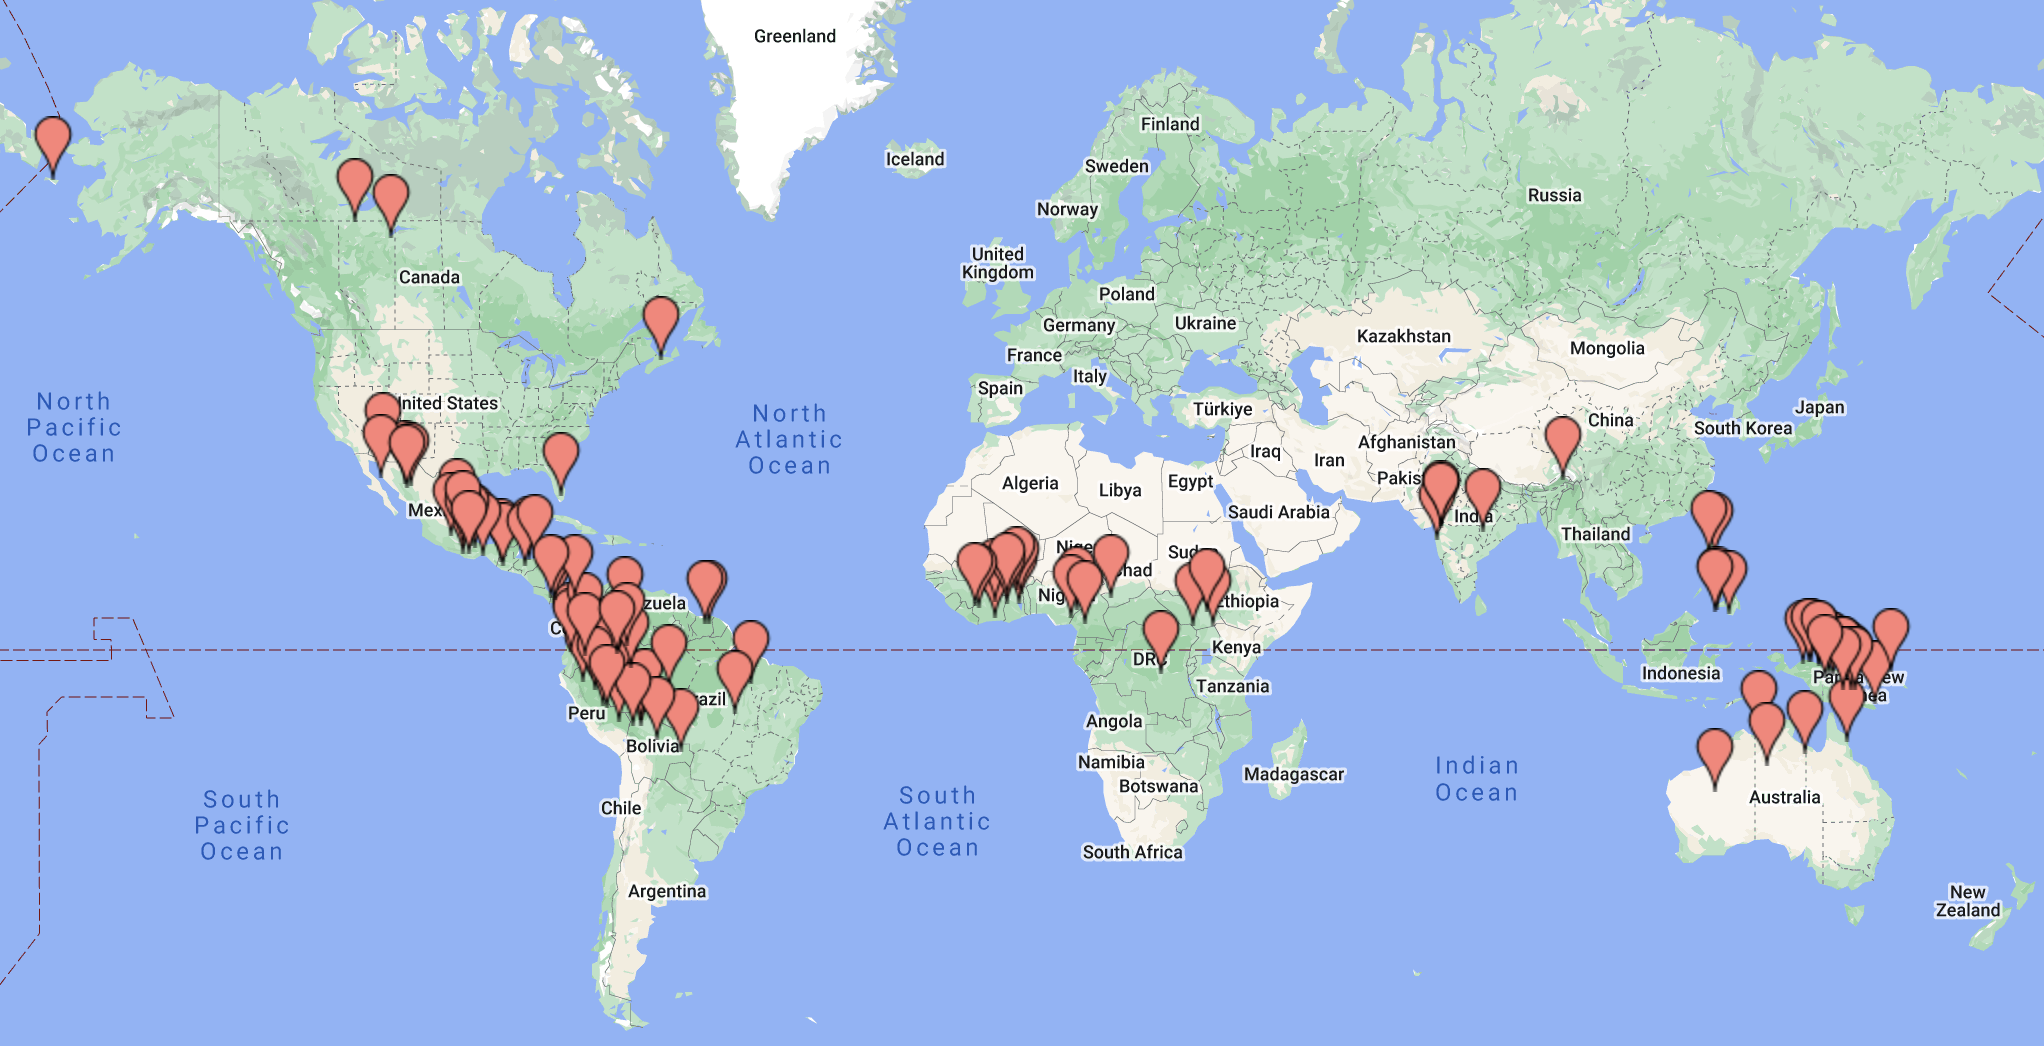
\includegraphics[width=\linewidth]{images/wcs-locations.png}
\decoRule
\caption[WCS Locations]{World map with information on the location of the 110 languages examined in the WCS.}
\label{fig:wcs-locations}
\end{figure}


In the World Color Survey (WCS - 1976 to 1980) data sets of 110 unwritten languages (See locations in Fig. \ref{fig:wcs-locations}) were collected, which were considered to be uncontaminated by contact with highly industrialized cultures 
\parencite{kayWorld2016}.
The procedure was twofold and the collection of Munsell chips was expanded by one white color chip. 
In a first ``free naming task" the participants were presented with each single Munsell chip in a pseudo randomized order and requested to name the respective color using a BCT. From these answers a list of unique BCT were elicited for the second ``focal task". Here participants were asked to name for each unique color term the chip that best represents the color term. This vast data set was then subject to many different analysis approaches.

% Lindsay & Brown (2006) - Universality of color names
\textcite{lindseyUniversality2006} used k-means clustering, taking the naming pattern of each of the WCS participants as input.
This analysis revealed successively forking categories from two to ten.
The step wise results resembled with exceptions very well the actual categories present in the examined WCS languages and English.
In addition, they identified regions of low concordance dividing roughly warm and cold colors across participants in color space.
Both findings indicate consistent tendencies across languages dependent on the number of color terms.

% Regier B&K (2007)Color naming reflects optimal partitions of color space

\begin{figure}[htbp]
\centering
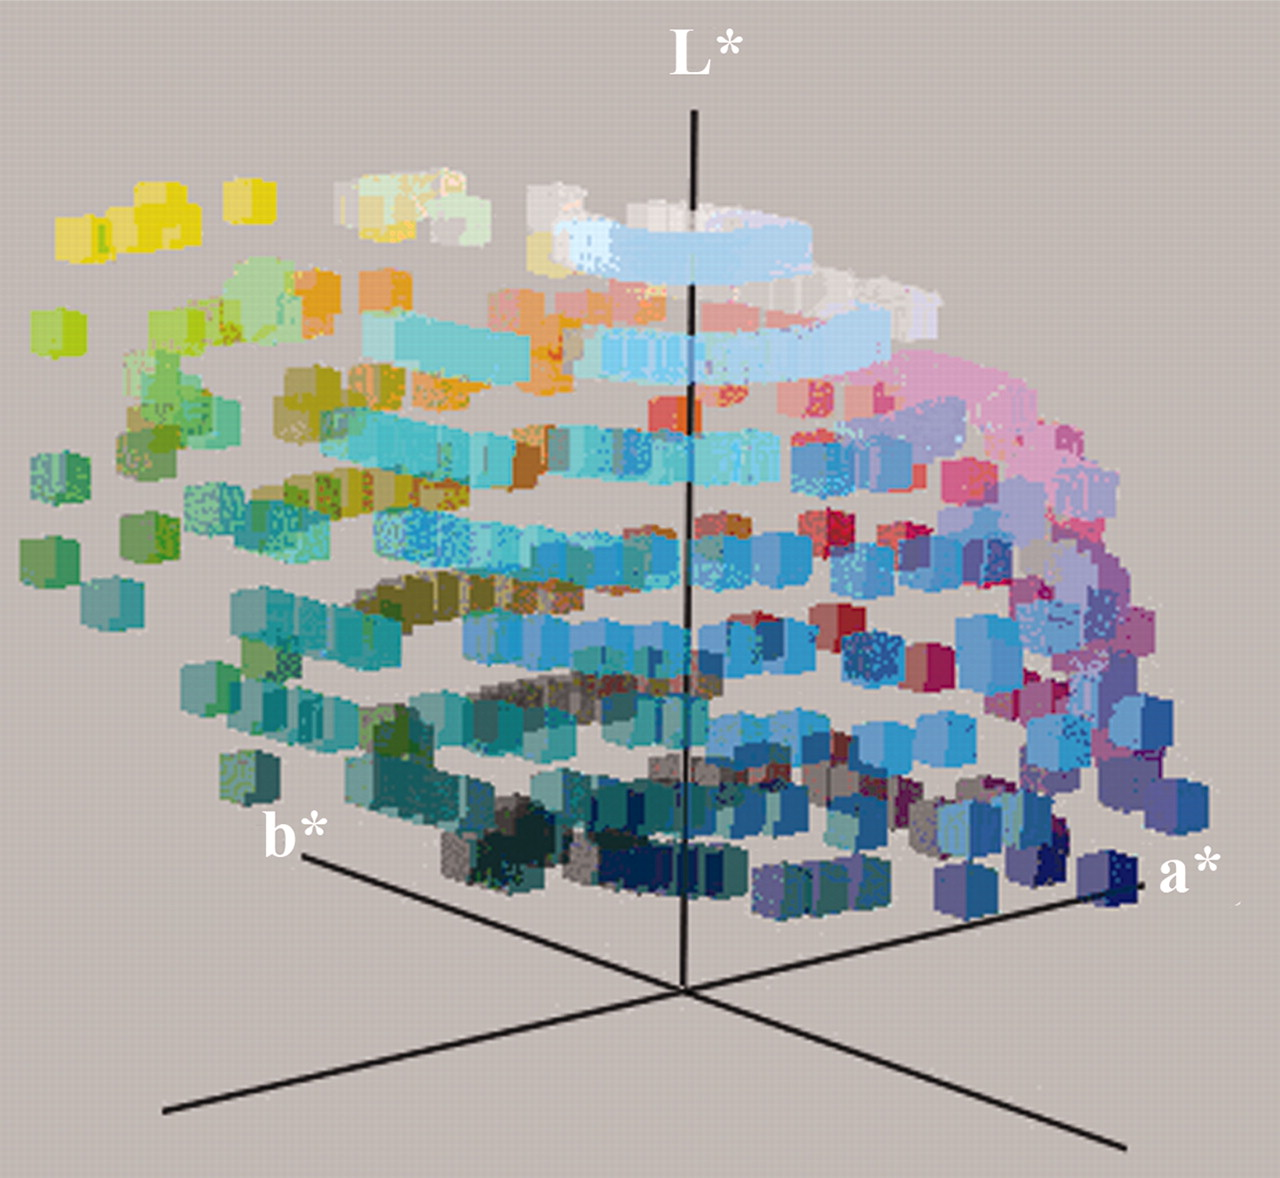
\includegraphics[width=\linewidth]{images/Cielab-space.jpeg}
\decoRule
\caption[Munsell Chips in Cielab Color Space.]{Munsell Chips in Cielab Color Space: 330 Musell color chips projected into Cielab color space. The irregular arrangement of the color chips is most prominent in the yellow region. \textcite{regierColor2007} used this irregularities and principles of categorization to explain the location and shape of color categories.
Taken from \textcite{regierColor2007}.}
\label{fig:Cielab_space}
\end{figure}

Subsequent theoretical work provided an alternative interpretation of the WCS findings. According to \textcite{regierColor2007}, the results of the WCS can be explained from two principles: a) a universally shared visual system, and b) an ``efficient'' organization of the lexicon based on the mere irregularity of color space and basic assumptions of categorization.
When converting the 330 color chips into the CIElab space, which constitutes a better psychophysical representation of color space, the resulting locations of these color values do not yield a perfect symmetric shape (Fig. \ref{fig:Cielab_space}).
A model using euclidean distances between color chips and rules of categorization to minimize similarity across categories and vice versa was able to predict naming patterns of real WCS languages.
A well formedness factor was calculated as the sum of all distances of all chips of the same category and the distances of all chips that do not belong to the same category.
When rotating the naming pattern along the L*axis, meaning to change the region of categories in the CIElab color space, the well formedness factor declined.
This was also true for languages that did not match the optimal model predictions.
Overall, these results support the hypothesis that color categories fit into optimal regions arranged by the universal peculiarities of color space.



% Relativists:
The Sapir-Whorf hypothesis assumes that perception is determined by the categories and filters of language. This approach agrees with the idea that color terminology seeks for optimization but is based on different premises. Color terminology is considered to be shaped by the rules of language rather than by universal properties of the color domain.

% Noga:
% \parenparencite{zaslavskyEfficient2018}
Information Bottleneck (IB) theory posits that language evolution is driven by a dual imperative: a tendency towards simplification for ease of use, while concurrently striving for maximal precision in communication.
\textcite{zaslavskyEfficient2018} showed that the WCS languages achieve nearly optimal communicative efficiency in this trade-off between complexity and information loss.
Following the IB principles, they were able to predict the successive differentiation of the color categories depicted in WCS languages. 
Similarity in naming patterns across languages of equal number of color terms is based on the principle to maximize accuracy given a particular complexity.
The results of an iterated learning experiment performed by \textcite{xuCultural2013} are consistent with this communicative account. In the experiment, English-speaking participants were initially exposed to random assignments of color chips. Participants then generalized their responses to unseen chips after receiving some examples. The result of one participant was given to another participant, imitating cultural transmission in the real world. The systems of color terms produced by this process reproduced the structure of systems of color terms documented in the WCS.


% Color Term Evolution
Regarding Berlin and Kay's evolution hypothesis, followup studies declared to have found additional BCT for Russian \parencite{daviesBasic1994}, Greek \parencite{thierryUnconscious2009}, Turkish \parencite{ozgenTurkish1998} and German\parencite{zollingerWhy1984}.
Specifically, \textcite{winawerRussian2007} found disparities between Russian and English speakers not just in their color nomenclature but also in their ability to quickly and accurately distinguish between colors that belong to separate categories in one language but not the other.
\textcite{kurikiModern2017} have identified a large number of color categories that have evolved in Japanese in less than the last fifty years.
Another study by \textcite{lindseyColor2014} proposed the stabilization of new color terms in English.
Furthermore, they provide evidence for both the emergence \parencite{levinsonYeli2000} and partitioning \parencite{kayLinguistic1978} hypothesis, indicating that new color terms emerge both between existing color categories and through partitioning of old categories.
Across all WCS languages, \textcite{lindsey2009World} were able to categorize individual differences into six motives, reflecting the use of different subsets of BCT. The presence of two motives was replicated for English \parencite{lindseyColor2014}.

% Gibbson:
A large picture corpus investigation by \textcite{gibsonColor2017} addresses the incentives for developing new color terms.
They discovered that objects on pictures are more likely to be colored in warm colors compared to the background.
Secondly, they were able to show that people name warm colors with higher precision and more concise than cold colors.
From this they concluded that the frequency of usage represents an impulse to differentiate between colors and come up with new categories.
In a further part of the study they recruited Tsimane participants. The Tsimane is a group of indigenous farmer-foragers living in remote areas of the Bolivian Amazon basin who are considered to be relatively isolated form western cultural influence \parencite{mcdermott2016indifference}.
When confronted with artificial objects they exhibited a higher usage of diverse color adjectives compared to natural objects.
Thus, industrialization and the crafting of artificial objects using synthetic colors might drive the creation of new color terms.
These results show, that we can not be sure that previous data sets are not outdated by now. Collecting new data could be specifically interesting in terms of deciphering the mechanisms of color term development especially for language exposed to globalization effect.



% \paragraph{\textbf{Color terms}}
\subsection{BCT}
The definition of BCT is non trivial. The study of basic color term has long history and dates back to Homers study about color term usage of the ancient Greek people \parencite{homer2015odyssey} later analysed by \textcite{gladstone1877colour}.
The concept was strongly promoted by aforementioned work by Berlin And Key \parencite{berlinBasic1969}. In this thesis we define BCT to be commonly used in everyday life and not a compound word but a single word. Across the literature different explanations are given and different components are emphasized although this is a key factor to elicit comparable results (\textcite{kayWorld2009},\textcite{lindseyColor2014}). In fact, finding a definition that can be validly generalized across languages is a complex task. Some languages investigated during the WCS did not even have a word for color. In these cases experimenters were asked to use phrases like "How does it strike you eyes" \parencite{kayWorld2016}. In addition, the role and concept of compound words vary strongly across languages and make this definition less explicit. 
%In the case of Vietnamese it is not conclusively evident whether parts of a single word can be seperated by an "-" or if this already indicated that it is a compound word.


Another issue in the literature is the relationship between color terms and color categories. Often these two concepts are used interchangeably or mixed. However, this poses problems, particularly when inferences are made from color terms and their use on color categories. \textcite{lindsey2009World} for example applied a k-means clustering algorithm on each individual naming pattern to identify a reasonable distribution of color categories independent of the actual term assigned. These categories are then named by the most common color term for this category. Even if they justify the level of this threshold the value remains arbitrary and distinct terms might be unified in single color categories. Therefore, in the domain of color terms, clustering terms together is a strong unstable assumption. To avoid this loss of information, in this work we propose an alternative approach that does not commit to one category for each color. 
% Confusion of Color Categories and Terms
% A weakness in the studies mentioned so far is the confusion of color terms and categories.
% For the sake of clustering synonyms into one category the authors used k-means clustering to detect categories.
% However, we understand that in the domain of color terms, clustering terms together is a strong unstable assumption.
% Where to put the threshold to distinguish between two clusters?
% Especially in this research investigating the influence of language on perception we should stick to the actual color terms.
% Therefore, we propose that each color term should be treated as an own category.
% Hence, we strongly depend our analysis on color terms instead of clustered categories.


%! Author = jakobnieder
%! Date = 3.01.24
\section{WEIRD Participants}
\label{sec:weired-participants}

It is a long-standing issue that the vast majority of participants in research about human psychology and behavior are WEIRD participants. WEIRD is an acronym proposed in \cite{henrichWeirdest2010} that stands for Western, Educated, Industrialized, Rich, and Democratic. Statistics from 2008 show that research recruits 96\% of their samples from only 12\% of the world population. Apparently, this recruitment window is getting narrower as 64\% - 80\% of these participants are undergraduates in psychology courses \parencite{arnettNeglected2008}.

%Problematic inference that findings are universal
    Inherently, there is no problem with this habit of recruitment. However, it is crucial to consider that inferences are only valid for the population for which the sample is representative. Without justification, a generalization of the general human psyche is not necessarily valid. The Müller-Lyer illusion is an example from the visual domain that induces differences in perception between populations \parencite{müller-lyer}. Far too often, researchers thoughtlessly claim to have discovered universality in human behavior without having tested for diversity across subpopulations. \textcite{WardUndergradsEmployed1993} discovered significant differences even between undergraduates and employed American adults. This diversity can differ in magnitude and direction, depending on the research question \parencite{henrichWeirdest2010}.

%Variation possibly originates from diverse reasons:
    Adaptation to environmental conditions through behavioral plasticity and genetic processes can lead to these variations in behavior. Cultural evolution, for instance, has a fundamental impact on the environment of individuals. Firstly, invention of tools, technology, and other knowledge impacts the physiological environment. Second, the cognitive sphere is influenced by the creation of counting systems, written symbols, categories, and heuristics. Third, the social environment is designed by norms, institutions, and laws \parencite{henrichWeirdest2010}.
    %(S. 80 rechts)

    Taking this into account, it could be posited that WEIRD participants may even represent the least suitable subgroup from which to derive generalizations. In contrast to e.g. small-scale societies, WEIRD populations typically exhibits a pronounced division of labor, considerable engagement with books and television, and a childhood experience marked by minimal physical punishment yet substantial levels of praise. Crystalline families and a high degree of individualism are further characteristics \parencite{henrichWeirdest2010}.
    %(S. 80 links)

    Encapsulation and therefore behavioral separation between sub-populations can also have genetic origins as relative similarity might reflect shared genetic origin \parencite{roseShared1988}. However, this assumption was challenged by a study showing that the expression of genes still can lead to different phenotype \parencite{kimCulture2010}. In addition, natural selection is thought to favour onto-genetic adaptation, enabling humans to better adapt to their environments through non-genetic means \parencite{henrichWeirdest2010}. Overall, evolutionary theory frequently serves as the foundation for discussions on universals although it may offer arbitrary explanations for varied behaviors. 

Aim of this argument is not to prove all populations to be substantially different in all types of behavior. Indeed, in many domains, fundamental similarities can be found across all populations such as the ability to make music, learn a language and theory of mind \parencite{henrichWeirdest2010}. However, it tries to question the predominant inference to carelessly conclude from WEIRED people that represent a very narrow sample of the world's population on universals. In fact, science can only benefit from this criticism to further expand the body of evidence and provide a more comprehensive picture of human behaviour.

In the field of color cognition the world-color-survey certainly was a pioneer project. Not only the sheer size of the dataset is impressive and makes it the most influential study related to color terms. The languages examined in the WCS all came from non-industrialized cultures and unwritten languages. Other studies tried to broaden this picture for languages which are spoken by many speakers such as English \parencite{lindseyColor2014}, Spanish and Chinese \parencite{xuComparison2023} and Russian \parencite{winawerRussian2007}. However, there is still a lack of completeness in this area of languages form industrialized and globalized countries. With the help of a new crowd-sourcing approach, in which we conducted online experiments worldwide, we were able to collect data from 25 mostly industrialized countries. In this way, this research can help close this long-standing knowledge gap and complete the picture.




% Example visual perception
    %when even the effect of carpentered corners have such an strong effect, we suspect that this might even stronger for the phenomenon related to language.
    %S. 64
%Even differences within the population of american participants.
    %From there they even go ahead and show fundamental differences between the broad amarican polulation to the psychology undergraduates... and childere
    %S(76)
%Also similarities detected(S. 78)
%Evolution theory often basis on which universals discussed but this can have arbitrary explanations for different behaviour.
    %also onto-genetic adaptation suspected to be favored by natural selection to make human capable of adapting non-genetically on environment.
%criteria to anticipate universality
%Strategies to change this habit.
    %institutionalized incentives.
    %Both from research institutions and publication side.
    %setting up testing facilities at but terminals, rail stations or airports
    %we got much better solution to this!


% Such as genetic, cultural, or environmental.
% In the context of color naming, the most prominent example is the difference between the English and the Himba language.
% The Himba language has only five color terms, whereas English has eleven.
% \parencite{sturgesStudies1969}
% This difference is often explained by the fact that the Himba language has no word for blue.
% \parencite{berlinBasic1969}
% This explanation is based on the Sapir-Whorf hypothesis, which states that the language we speak influences the way we perceive the world.
% \parencite{whorfLanguage1956}
% This hypothesis is controversial and has been criticized for its lack of empirical evidence.
% \parencite{regierColor2007}
% Nevertheless, it is still a popular explanation for the differences in color naming patterns between languages.
% \parencite{regierColor2007}



%This is especially important in the context of color naming because it is often used as an example of a universal phenomenon.
%\parencite{regierColor2007}


\section{Online Experiments}

The term crowd-sourcing emerged analogously to the term outsourcing, which describes the process of relocating production locations to other countries mostly with lower production costs. The initial idea of crowd-sourcing was to recruit groups of internet users to complete human intelligence tasks (HITs), instead of hiring temporary employees. These tasks can vary from commercial applications such as attaching meaningful tags to numerous products of a new online shop to cleaning up training data for machine learning or spectacular database investigations \parencite{CrowdsourceML,TurkRescue}. Specifically, these are tasks that are too complicated to be solved by computers and need human intelligence but do not require skilled personnel \parencite{BerendViabCrowd2011}. 
%Crowd sourcing can be defined as “the intentional mobilization for commercial exploitation of creative ideas and other forms of work performed by consumers” \parencite{def-crowdsource}. 
Importantly, crowd source workers are paid, recruited from any geographic location and hired only for single tasks. 

In recent years it has been discovered that especially science can benefit from this new approach. Online experiments offer the opportunity to collect very simple, flexible and fast data from a large pool of participants \parencite{BerendViabCrowd2011, truellResponse2002}. Reduced costs, easier logistics, and lower investment of physical resources are other advantages of online experiments \parencite{KrautOnlExpCost}. But the most significant benefit offered by conducting experiments online is the potential to surmount the prevalent reliance on a participant pool characterized as WEIRD. Online participant pools are found to be older as well as more ethnically and educationally diverse and thereby may help to enhance the diversity and representativeness of research samples \parencite{BerendViabCrowd2011, henrichWeirdest2010}. Earlier studies have also shown that the pools of online providers such as Mechanical Turk are more representative for the average working adult population within a country \parencite{BerendViabCrowd2011}. This is crucial as \textcite{WardUndergradsEmployed1993} has indicated even significant differences between undergraduate and employed American adults.
% At the same time data are still similar to the ones obtained from undergraduate students and are reported to have comparable quality to in lab experiments \parencite{BerendViabCrowd2011, sprouseValidAMazTurk2010}.
% providers

%MTurk
The first relevant provider that offered the opportunity to recruit participants online was amazon mechanical turk (MTurk, \parencite{mturk}). In 2015 MTurk generously claimed to have 500,000 online workers available, which was corrected down to 7,300 actually recruitable participants, which is still a large participant pool \parencite{stewartAverage2015}. Although the platform was not intended to host research surveys, in 2015 already 1,200 studies were conducted online. Some of these studies replicated results from older lab studies and therefore proved consistency across the procedures \parencite{CrumpEval2013, AmirEcoGames2012, hortonOnline2011}.

%Prolific
However, several problems related to the pool management of MTurk were discovered. This got addressed by Prolific \parencite{prolific} which is currently the predominant recruiter used for online experiments providing access to a pool of currently 120,000 participants from 35 countries %(almost all from the OECD-list).
In contrast, Prolific was specifically designed for research surveys and informs participants accordingly. Again comparable results show consistency with Mturk \parencite{peerTurk2017}. Prolific ensures fair payment, and gives incentives for participants to provide qualitative answers. The participant pool is even more geological and ethical diverse and the website design allows to target participants based on demographic criteria. Each participant is strictly identified to ensure that each person can only participate once and to exclude bot participants. Conversation between experimenter and participants is monitored by Prolific to prohibit demand effects and exploitation \parencite{NeckaMturkProblematic2016}.

% Lucid
The geographical reach of Prolific predominantly encompasses countries listed by the OECD, which implies that surveys carried out through this platform are largely confined to industrialized nations. Conversely, Lucid \parencite{lucid} serves as an alternative marketplace, covering a broader spectrum of 112 countries and 73 languages that include both industrialized and non-industrialized regions, offering a more diverse participant pool. Importantly, participants on Lucid are approached using their own native language whereas all communication on Prolific is in English.
This opens up new possibilities to reach an even broader pool of participants around the world. To our knowledge, this is the first research survey to use Lucid as a recruiting platform and to take advantage of some of this potential.
The task was not only to identify the recruiting mechanisms of this platform, but also to evaluate its consistency compared to established platforms such as Prolific.




% Lucid is not tailred towards research

% Both recruiters allow the use of individual software to acustom the surveys






% Because of poor participants moderation the quality of this provider declined \parencite{Kennedy_Clifford_Burleigh_Waggoner_Jewell_Winter_2020}.
% Since then a commonly used provider is Prolific. 


% Loss of nativity:
% - participation in hundreds of studies may have a practice effect.
% - Dicussion board organizes exchange between MTurk workers
% - Conversation can be monitored but not controlled 
% No controlled in lab experiment conditions
% - Multitasking (watching TV or listen to music Chandler et al. (2014)Necka et al. (2016)
% - No substantial differences between groups found Necka et al. (2016)
% - Caution for experiments if design requires stable conditions across participants
% Payment:
% - Ethical problems in the case of exploiting participants by paying to less as well as overpaying and therefore luring them into participation of experiment they would not do for lower wage. Shank, 2016; Crump et al., 2013; Mason and Suri, 2012)
% - Although data quality seems to be independent from reward size it might still have a arbitrary influence on the data quality (Buhrmester et al., 2011)
% Participant IDs:
% - Tracking of participants that use multiple accounts and therefore participate more than once in the survey
% - (Chandler et al., 2014).
% Demand effect:
% - To maintain high data quality the experimenter is able to give feedback or even reject the payment of participants according to the answers of a participant. The feedback results in an acceptance score assigned to each participant wich can then lead to exclusion to certain surveys. 
% - To avoid low ratings participants might give answers according to how they expect the results of the survey are.
% - Necka et al. (2016)


% Prolific:
% 1.2 dedicated research pool:
% - explicetly recruits participants for research and informs them accordingly.
% - Study have replicated results of experiments conducted on Mturk
% - Reported a geographical and ethnical more diverse pool

% 2. Subject pool management:
% - Ensure fair payment by setting a minimum fixed payment of 5 GBP per hour.
% - In fact this might be problematic in case of developing countries as it is considered unethical to offer excessive incentives to lure participants into studies
% - Transparent information of the duration of a experiment
% - Communication between provider and participant is mediated by Prolific. 
% - Rejection of low quality data have to be justified by the experimenter and participants can raise an objection in case.
% - This lowers the danger of demand effects that the participant answers as he thinks he is supposed to answer.
% - In addition participant always can terminate or return their submission without fear of negative reputation 
% - Very good participants can even win prizes
% - H

% 3. Pre-Screening:
% - Experimenters can exclude participants based on pre screening questions. 
% - To mitigate the risk of response bias, where participants might answer based on perceived expectations, basic demographic information is collected at the account creation stage. Furthermore, these responses are stored and made available for subsequent experiments, ensuring consistency and reducing the need for repetitive data collection.

% 4. Exclusion of individual participants
% - Prolific employs a system where each participant is assigned a unique participant ID and monitors their activity on the platform. This approach enables the prevention of individuals from participating in the same experiment more than once, ensuring the integrity of experimental data.


\section{Study Significance}

This thesis intends to contribute to science on multiple frontiers. Methodically, the use of online experiments generally helps to expand the circle of participants and to be able to make more representative statements about the human psyche. 
The preponderance of psychological research continues to draw from a limited and unrepresentative sample—predominantly from WEIRD societies, which has been shown to inadequately reflect the diversity of the global human population.
This is even leveraged by the use of Lucid as an recruitment platform offering a wider range of accessible countries and languages than traditional recruiters. Since this is the first research program to use this recruiter, it is not only taking advantage of the new potentials but also explores the mechanisms of recruitment on this platform. By doing so we set the way for further research exploiting these massive potentials.
In this study, we tested 4,351 participants of 25 languages across three continents Europe, Asia and Africa.

In the domain of color terms, this study closes an important knowledge gap that has existed for a long time. 
Under the assumption that globalization effects diminish differences across languages a lot of research was done investigating unwritten languages of small scale societies.
Conclusions derived from these data sets could only examine the developmental mechanisms in these environments.
Further studies investigated single industrialized languages, but varied in methodology and the availability of data sets and therefore do not allow comparison.
The data set obtained covers a range of 25 mostly industrialized languages and recruited participants fully exposed to cultural exchange through the Internet.
Using the data set obtained, we are now in a position to examine the effects of globalization on the contingent of color terms in industrialized languages.

With growing capabilities, LLMs are becoming more and more important in the daily lives of Internet users around the world. This also increases the importance of understanding how they work. Do they simulate human behavior or operate more independently?
Conducting experiments analogously allows to determine the relationship between human and GPT4 behaviour. Even more importantly, LLMs can help determine whether the perceptual world can be inferred from language.
In the context of this study, GPT4 is considered to be a multilingual agent highly exposed to cultural exchange, functioning as a control group.



\chapter{Methods}
\section{Experiment}

\subsection{Procedure}
 In the experiment 4,351 participants had to fill out custom demographic questions on the Lucid website. In order to qualify, the participant had to satisfy all of the following criteria: brought up monolingually, hold nationality of the country we targeted, speak the language as a native and use it as their first language.

In the first page the participants are presented with a consent page. Here they accept the conditions of privacy and data collection. The first part of the experiment is Wikivocab (See Sec. \ref{wikivocab}), a pre-screener test to determine the participant's proficiency of the examined language. Subsequently, the participants had to pass the main experiment. Here they were presented with a color square (See Sec. \ref{stimuli}) which they had to name with a basic color term (See Sec. \ref{paradigm}). After completion of all trials, the participants where forwarded to a color blindness test (See Sec.\ref{col-blindness}). At the end of the experiment, the participants were asked about the duration of any training in music and art related activities.

\subsection{Software Implementation}
The Experiment was implemented using Psynet \footnote{\url{https://www.psynet.dev}}. Psynet is a framework built on Dallinger which is a platform to host and deploy online experiments \footnote{\url{https://github.com/Dallinger/Dallinger}}. It allows you to develop and design complex experiments \parencite{harrisonGibbs2020}. We recruited participants from two different crowd-sourcing platforms: Prolific \parencite{prolific} and Lucid platform by Cint \parencite{lucid,cint}. \textcite{lucid} is a platform for recruiting human participants serving as an exchange to connect survey providers and recruting services, which was acquired by the major recruiting firm Cint (\cite{cint}) in 2022. Currently, Cint offers Lucid as one of its services. In this thesis, we refer to the platform as `Lucid' to distinguish the participant group it provides, which may vary from the broader pool available through Cint. The attendees interact with the study via a user interface in their browser. This interface connects to a Python EC2 Server (Amazon Elastic Compute Cloud) cluster on the back end, overseeing the experiment's progression. Additionally, there's a secure Postgres database set up for storing data. To keep the interaction and loading time for the participants low, EC2 servers were provisioned at locations close to the participants location. The availability of the code detailing the experiments is specified in section \ref{code_availability}.

\begin{figure}[htp]
    \centering
    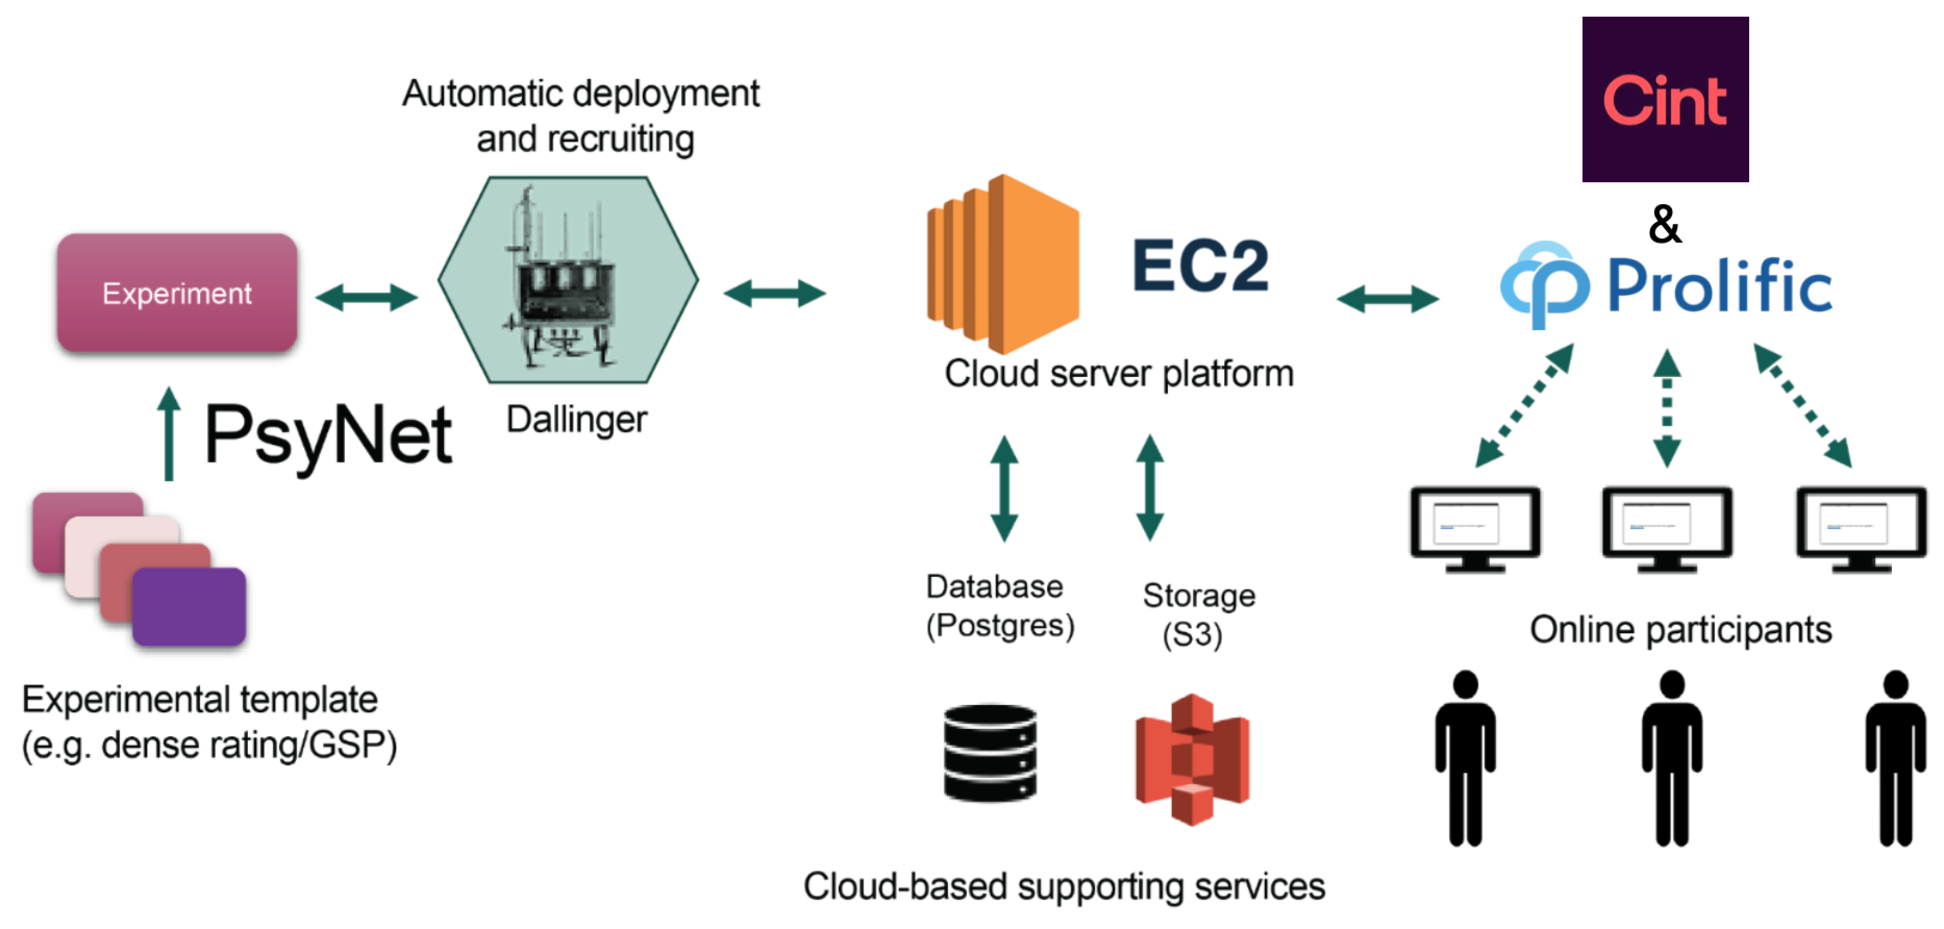
\includegraphics[width=\textwidth]{psynet-workflow.pdf}
    \decoRule
    \caption[Structure of the data collection infrastructure]{Structure of the data collection infrastructure: Reproduced from Harrison et al., 2020 and updated with more recent deployment platforms Prolific and Lucid.}
    \label{fig:psynet-workflow}
\end{figure}

To counter the arguments that online experiments have a lack of control over the experimental conditions and that participants respond honestly, Psynet offers a range of pre-screen test such as Wikivocab and a color-blindness test.


\subsection{Wikivocab}
\label{wikivocab}
Wikivocab is a pre screen test developed by \textcite{vanrijnWorld2023} to predict the proficiency of participants in languages. It was shown that the test is reliable and can distinguish speaker of closely related languages. The procedure is still under development. By the time we conducted the experiments it supported 36 languages covering all examined languages except Thai. For this test low frequency words are sampled from the Wikipedia corpus as real words. Second, pseudo words are created using an algorithm that preserves the phonotactic structure of the language. The participants are then asked to identify the real words. The test is designed to be language independent and is therefore suitable for a each specific language (Fig. \ref{fig:pre-screens} B).


\subsection{Color Blindness Test}
\label{col-blindness}
The color blindness test of the Psynet framework adapts to the procedure of the Ishihara-color-blindness test \parencite{clark1924ishihara}. An image shows circles of diverging size. Some of these circles are colored such that their connected overall picture shapes a number. Importantly, the used colors and contrasts are designed such that for participant suffering from color perception deficiencies it is hard to distinguish between background and number. Each participant was presented with six trials and had to give at least four correct answers. Participants with a smaller score where excluded from the analysis.
(Fig. \ref{fig:pre-screens} A)

\begin{figure}[htp]
    \centering
    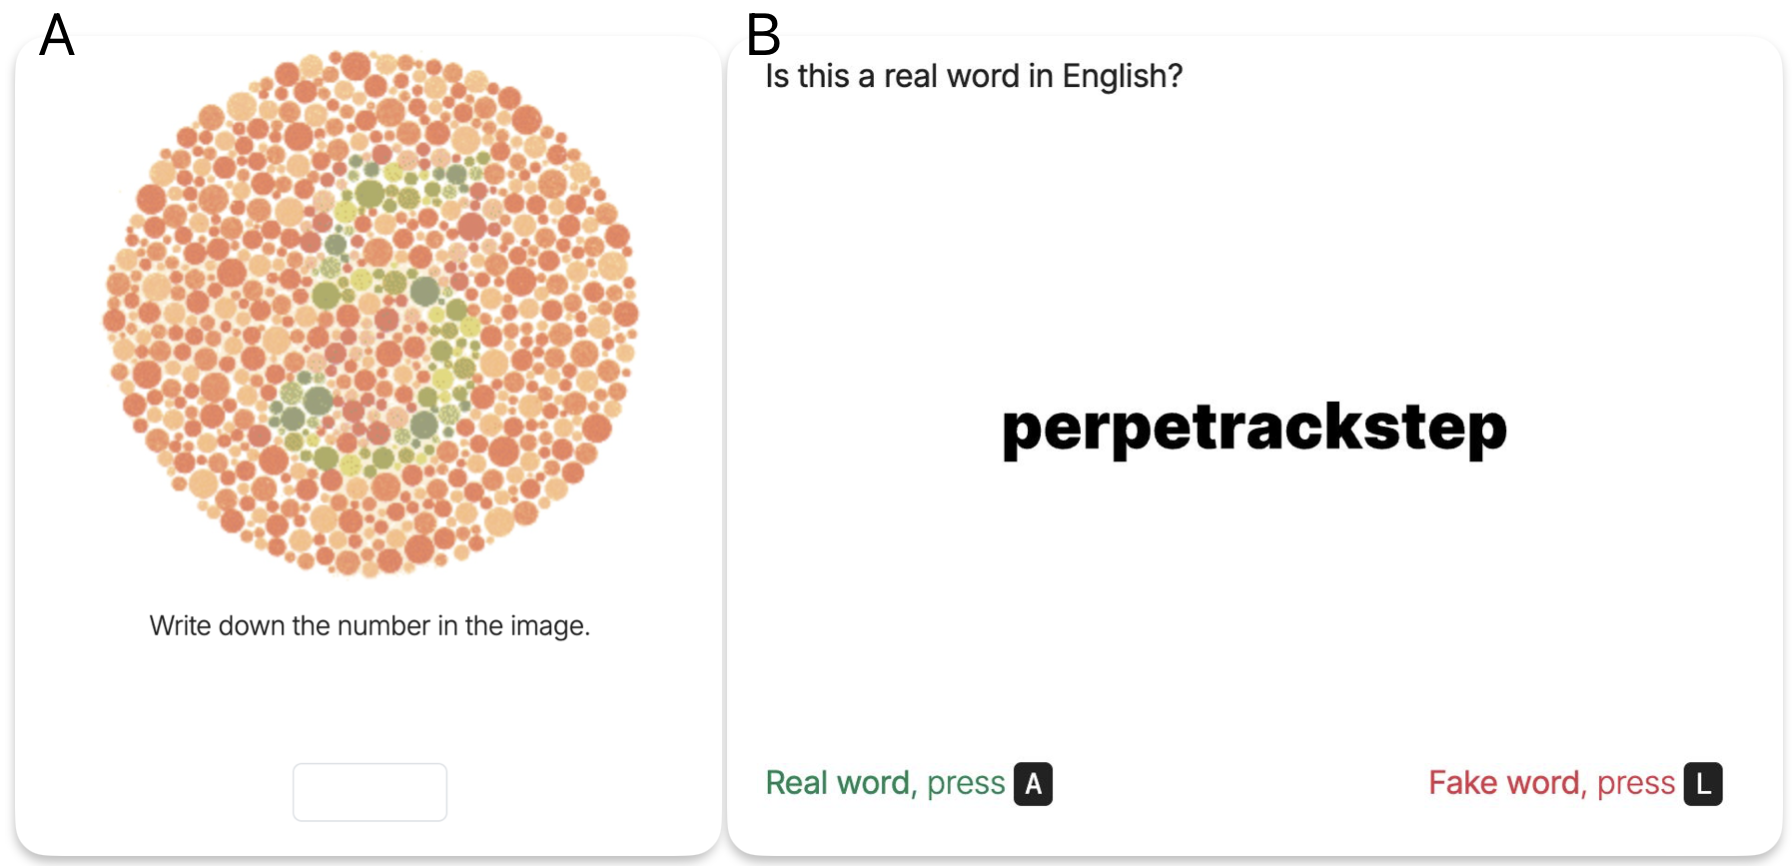
\includegraphics[width=\textwidth]{images/PrescreenTests.png}
    \decoRule
    \caption[Ishihara Color Blindness Test and Wikivocab]{Ishihara Color Blindness Test and Wikivocab: A: Color blindness test adapted to the Ishihara procedure asking participants to report the depicted number. B: Wikivocab trail showing a generated pseudo-word. Participants were to detect real and artificial words.}
    \label{fig:pre-screens}
\end{figure}



\subsection{Paradigm}
\label{paradigm}
There have been multiple paradigms applied in the field of color categorization such as color discrimination \parencite{winawerRussian2007}, serial reproduction \parencite{xuCultural2013}, and similarity judgments \parencite{marjieh2023words}. This study aimed to collect comprehensive up to date color lexicony of a large number of languages. Therefore, we decided to adapt to the free naming task of the World Color Survey \parencite{kayWorld2009}. Participants were asked to freely name presented color patches.

To prevent fatigue, each participant was only presented with a subset of 50 color chips instead of the full 330 chips. To make the prompt generalizable and simple to translate into all languages and give unambiguous guidelines about BCT, we converged (after piloting different options, and comparing different prompt from the literature) on the following: 

“Please identify the color above using a commonly used color name. The color name should be the one you would normally use in everyday life to describe that color. Avoid using compound words. The color name should be a single word”. 

\begin{figure}[htp]
    \centering
    \fbox{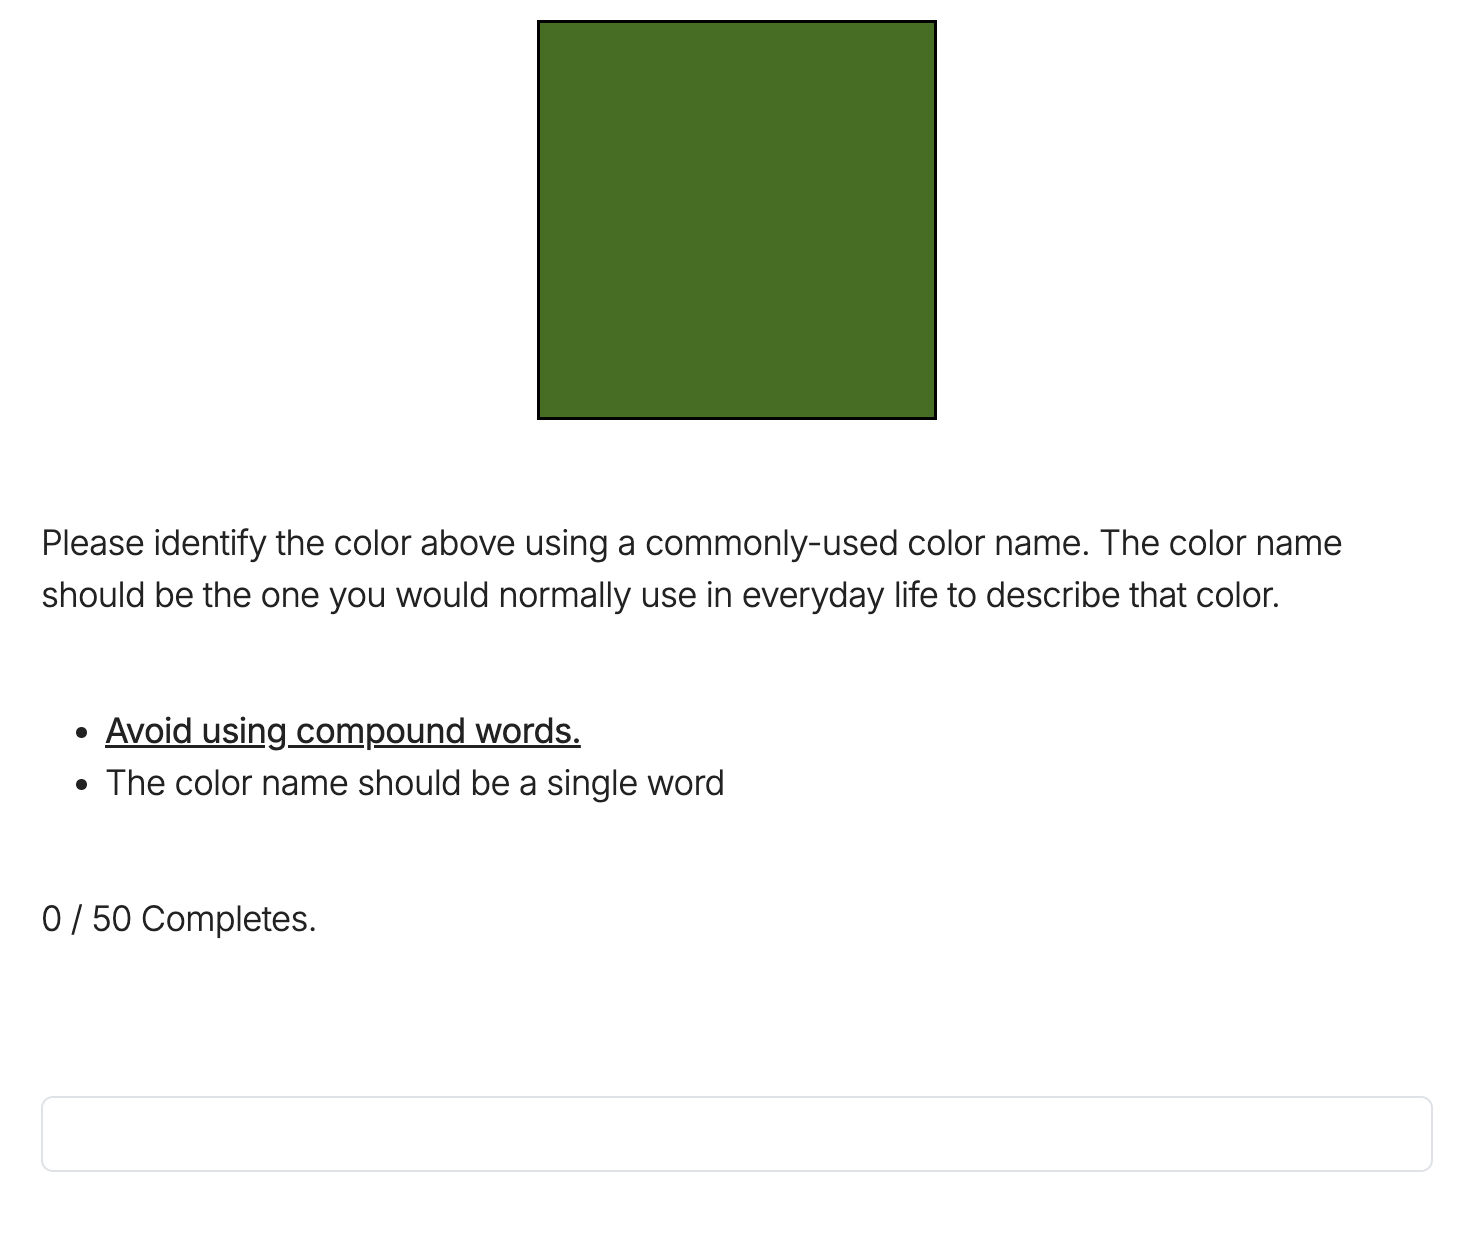
\includegraphics[width=\textwidth]{images/Color-Trail.png}}
    \decoRule
    \caption[Color trail]{Main task of the experiment, presents a square of color to the participant and requests the participant to name the color. The input had to fulfill the following requirements: Min and max number of characters obtained from data elicited from GPT4, only in the language commonly used scripts allowed, no digits, no spaces.}
    \label{fig:col-trail}
\end{figure}


The prompt was then translated by professional translators recruited with the online service translated \parencite{translated} to all 25 languages (Fig. \ref{fig:deployment_map}). Translated was fully paid by the service for their translation service.
%Overall, we collected 121,108 naming responses from the participants.


\subsection{Stimuli}
\label{stimuli}
To ensure comparability with the literature we adopted to the concept of subdividing the color space into 330 color chips \parencite{kayWorld2009}. Color space was divided into eight levels of lightness and 40 equal steps on the hue scale. This collection was complemented by 10 achromatic Musell chips ranging from black over gray to white (Fig. \ref{fig:mode_prop_maps} upper panel).
% (Fig. \ref{fig:munsell-chips}).

For the representation of colors we used the RGB color space which is based on the idea of trichromatic vision. The human eye has three types of cone photoreceptores that are most sensitive to different ranges of wavelengths. Short, Medium, and Long. These correspond roughly to the blue, green, and red parts of the spectrum, respectively. In the brain the impression of all shades of colors gets constructed through the relative excitation of these three types of cones. In digital image processing this fact is used to display every shade of each color by mixing the amount of red, green or blue for every pixel \parencite{rgb-model}.


% \begin{figure}[htp]
%     \centering
%     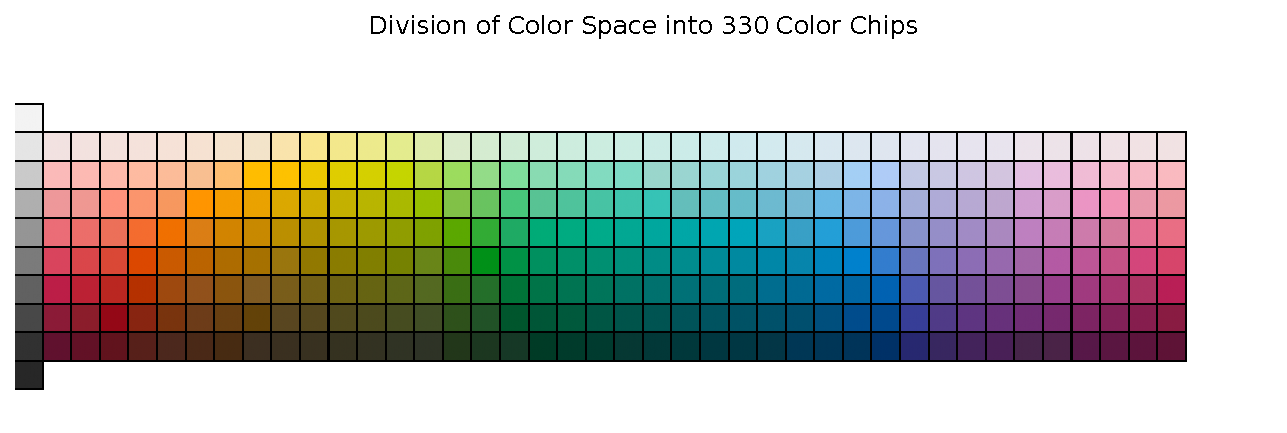
\includegraphics[width=\textwidth]{images/munsell_chips.pdf}
%     \decoRule
%     \caption[330 Munsell-Chips]{330 Munsell-Chips: Color space equally divided along hue and lightness axis (40x8).}
%     \label{fig:munsell-chips}
% \end{figure}

\begin{figure}[h!t]
\centering
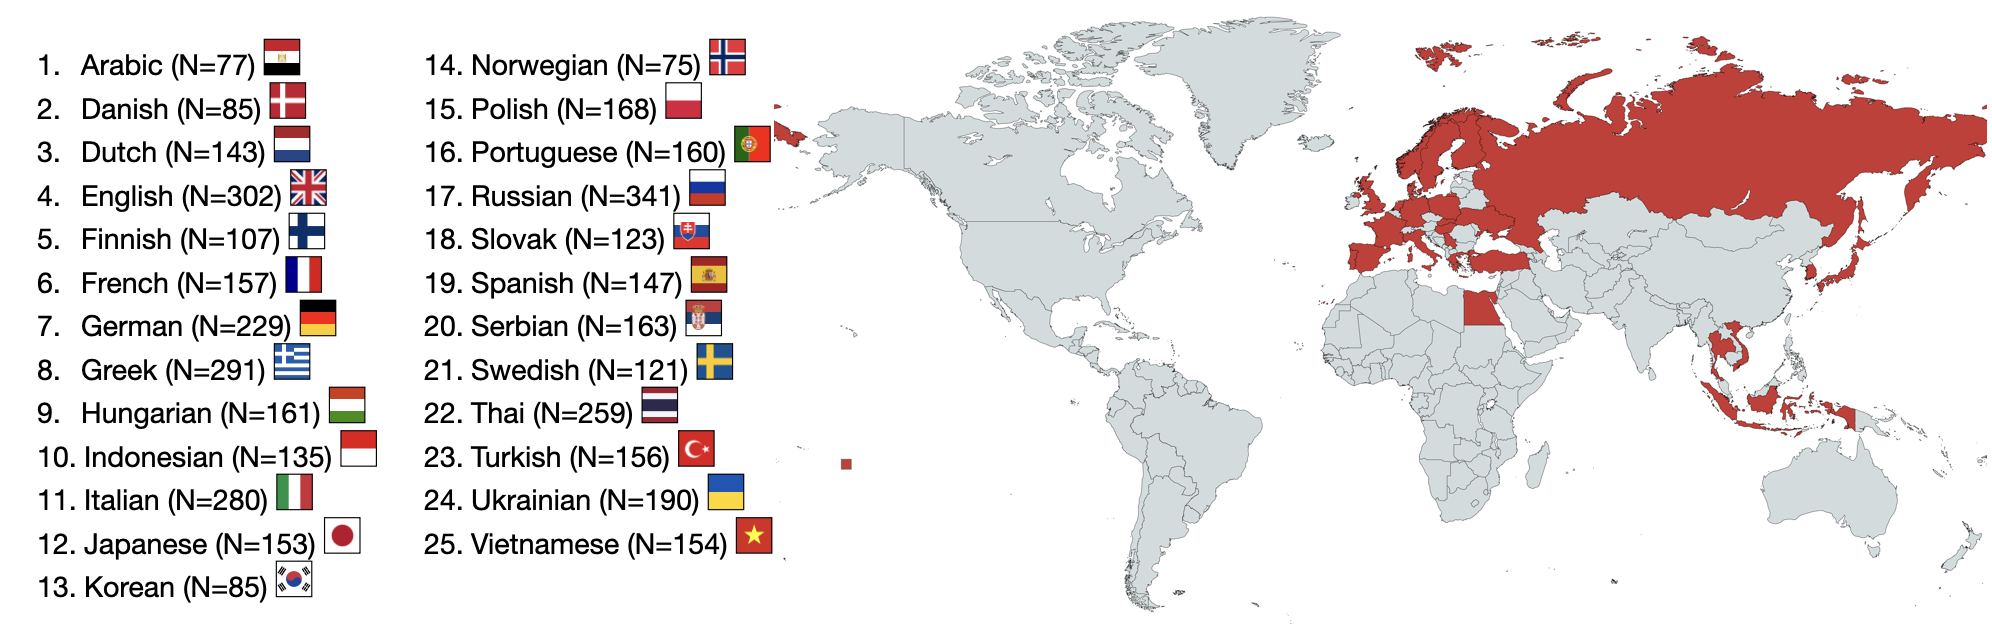
\includegraphics[page=1, width=\linewidth]{images/deployment_map.png}
\decoRule
\caption[Deployment Map]{Deployment Map: Regions in the world we recruited participants from.}
\label{fig:deployment_map}
\end{figure}


\section{Participants}
\label{sec:participants}
All participants provided informed consent according to an approved protocol (Max Planck Ethics Council \#2021\_42) and were recruited through Prolific \parencite{prolific} and Lucid Marketplace \parencite{lucid}.
Data were collected from 29 groups (25 in Lucid and 4 in Prolific, with 25 unique languages, see Figure \ref{fig:deployment_map}). 
Per group between 75 and 259 participants were recruited (mean: 150.0, sd=39.6). We aim to recruit about 160 people per group and at least 75 per group. The number of participants was matched to previous literature and our pilot data. Importantly, the difficulty (time to recruit) was different across locations. This resulted that the number of participant varied from location to location. We recruited the data in two batches: one in Summer 2023 (from 13/06/2023 - 10/8/2023) and one in early 2024 (from 11/03/2024 - 15/03/2024). 
Altogether, we collected data from 4,351 participants (Lucid: 3,834, Prolific: 517).
The mean age across all participants was 42 (sd=15) and the male to female ratio was 38.5 \% female. Participants had in average 1.5 (sd=3.6) years of formal training and 2.0 (sd=6.2) years of non formal training in the field of color related activities. 
For all languages the wikivocab score was very high, in average 80\% right answers.
The wage per hour was adapted to the local minimal wage.  Summary information about all recruited groups can be found in Table \ref{tab:pgfplotstable_csv}.


\begin{sidewaystable}[htp]
\centering
\resizebox{0.9\textwidth}{!}{%
    \pgfplotstabletypeset[
        col sep=comma,
        string type,
        every head row/.style={before row=\hline, after row=\hline},
        every last row/.style={before row=\hline\hline, after row=\hline},
        every first column/.style={column type=|l},
        every last column/.style={column type=l|},
    ]{images/participants_table.csv}
}
\caption{Participants}
\label{tab:pgfplotstable_csv}
\end{sidewaystable}


% HERE YOU MAY WANT TO PROVIDE INFORMATION ON THE GPT EXPERIMENTS BECAUSE DATA CLEANING IS UNCLEAR IF YOU DON"T KNOW ABOU THESE EXPERIMENTS.
\section{GPT4 data collection}
In a second experiment participants were replaced with a LLM.
Here data collection was done by Dr. Ilia Sucholutsky analogous to the elicitation of the human data. As an LLM, OpenAI's GPT4 \parencite{achiam2023gpt} was examined using the Microsoft Azure OpenAI API (version 0613 of the model).
Data collection was performed with the default value of the hyperparameter temperature = 0.7.
Consolidating GPT4 via the API enables two steps of prompting. The system prompt is used to prepare the model for the experiment: ``Follow all instructions that users provide to you in their own language. Respond to users in their own language using only a single word and no other text. Do not use any compound words.''
For each languages we then used the exact same elicitation prompt we used for humans translated into the respective language. For GPT4 instead of showing the visual color we specified the colors as hexcodes: 

``COLOR: $<$hexcode$>$
Please identify the color above using a commonly-used color name. The color name should be the one you would normally use in everyday life to describe that color. Avoid using compound words. The color name should be a single word.'' 
50 responses per color chip for each language were collected.

The LLM-V dataset was obtained through the utilization of OpenAI's GPT4-V (version GPT4-vision-preview, accessed via Microsoft Azure's OpenAI API), employing a methodology consistent with the one previously delineated. However, instead of providing GPT4 with a hexadecimal code, the process involved the presentation of a Base64 encoded image representative of the specific color.


\section{Data Cleaning}
The paradigm used in this study elicited free text. Therefore, we had to clean these results in several steps. The main problems appeared to be invalid answers, inconsistent use of grammatical forms, diacritics, special scripts, compound words and typos. The data cleaning was done in the same manner for humans and GPT4 data.


\subsection{Exclusion of invalid answers}
The first step in the cleaning pipeline was to exclude invalid answers such as "Error", "Nan", empty answers, answers containing spaces, digits, punctuation, only capital letters as we assumed them to be acronyms, or if scripts were used which are not common in the respective language. This can also occur when GPT4 and human did not provide valid responses and thus this "empty" response needs to be eliminated from further processing.
Exclusion of unusual scripts was done by first identifying the Unicode blocks\footnote{\url{http://unicode.org/Public/UNIDATA/Blocks.txt}} of the responses and then counter check if these are present in a list of scripts we specified beforehand.

\subsection{Lemmatization}
For languages under support (excluding Arabic Japanese, Serbian, Thai and Vietnamese), we applied lemmatization \parencite{jurafskySpeech}\footnote{\url{https://pypi.org/project/simplemma/}} . In order to group the same words together, different forms of the same term get "reduced" to its root or lemma. This is more elegant than other methods, such as stemming.

\subsection{Diacritics}
Some languages include the use of diacritics in their alphabet.
However, the participants did not use these diacritics consistently. 
To match the versions of each color term with and without diacritics, we removed them and then replaced all occurrences with the most common version. 
This was done using the python unicodedata library \footnote{\url{https://docs.python.org/3/library/unicodedata.html}}.
Arabic is a special case where pronunciation has an impact on the written form of a letter, including diacritics. Therefore, different dialects can lead to modified writing and characters \parencite{owens2013oxford}. A list of letters were identified that are most exposed to this influence and unified across the dataset (\textarabic{ى, ؤ, إ, أ, ئ, ة} to \textarabic{ي, و, ا, ا, ي, ه}).


\subsection{Special scripts}
We regarded Japanese and Korean as employing "special scripts." 
Japanese incorporates three distinct scripts in its writing system: Kanji, which is logographic, and two syllabic scripts, Hiragana and Katakana\parencite{harai2007japanese}.
Participants seem not to use a single script exclusively.
To universalize the scripts, we transformed all answers into katakana using the pykakasi\footnote{\url{https://pypi.org/project/pykakasi/}} package.
The most common script in Korean is Hangul where single syllables are put together in blocks \parencite{pae2018korean}.
To decomposed different writings of the same words we syllabified all answers into their Jamos or components. We used for this purpose the jamotools\footnote{\url{https://pypi.org/project/jamotools/}} python package.
%This was done using the "jamotools" python package.

\subsection{Compound words}
To remove compound words we identified frequent color terms (occurring in >1\% of answers).
For all these words we iterated over all unique color terms and checked weather they end with that word. If this was the case and the two terms co occurred in the dataset we replaced the compound word with the base (e.g. "hellblau" -> "blau").
This heuristic assumes that in case of color terms compound words are built from a base which is the main color category referred to and a modulator part placed beforehand giving it a specified shade.
This was however not applicable to Arabic.

\subsection{Typos}
Typos were detected based on the frequency of a word in the respective language calculated using "thefuzz" library \footnote{\url{https://pypi.org/project/thefuzz/}}. If the score exceeds the threshold of 80 the color term was replaced with the most similar color term which was evaluated using the Levenstein edit distance and co-occurrence in the dataset.

\subsection{Rare words}
As a last cleaning step infrequent color terms (occurring in less than 1\% of all answers) where deleted from the dataset even if the exclusion of these color terms lead to the extinction of all answers for a color chip so that no data were left to name this color chip. If this was the case instead of deleting these color terms from the data they were mapped to one of the frequently used color terms they most co-occurred with in the data. 
\section{Data-Visualization}

\subsection{Mode Maps}

Mode maps are a common way to visualize the distribution of color terms in a color space (Fig. \ref{fig:mode_prop_maps} middle panel).
These visualizations display the 330 Color chips (Fig. \ref{fig:mode_prop_maps} upper panel) as a two-dimensional map of the color space, where the color of each chip represents the most common color term for that chip.
We innovate here a bit, by improving the standard visualization with the following trick. 
 For each chip, we assign it a color that is the average over all chips in that category.
%We visualize the selected color for each  chip by assigning it to a color which  is the average over all chips of this category.
%In this way the color of each term is calculated by taking the mean of all chips that were assigned to that term, and thus allow us to quickly see the selected visual category over the space of all chips.
 As a result, each term's color is calculated based on the mean of all chips assigned to it, allowing us to quickly see the selected visual category over all chips (See Fig.\ref{fig:mode_prop_maps} lower panel).
This approach is more informative than using generic unrelated colors for example in \cite{regierColor2007} (See Fig.\ref{fig:mode_prop_maps} middle panel). 
% In the case of ties, the term that occurs the most in the overall dataset wins.


%The characters '*' and '+' are used to indicate the proportion of the winning term in respect to the number of the total number of terms assigned to that chip.
%Therefore, they indicate a measure of confidence in the assignment.

\subsection{Proportion Maps}
We propose another new way of visualizing color lexicons and their distribution in color space.
For every chip our proportion maps show the distribution of the first three most common terms (Fig. \ref{fig:mode_prop_maps} lower panel).
This provides additional information and allows a more intuitive understanding of the centers and boundaries of color categories in color space. Importantly, it allows us to see better the overlap and boundary of color categories beyond only the most frequent color. 

% insert image that represents the mode map
% \begin{figure}[htp]
%     \centering
%     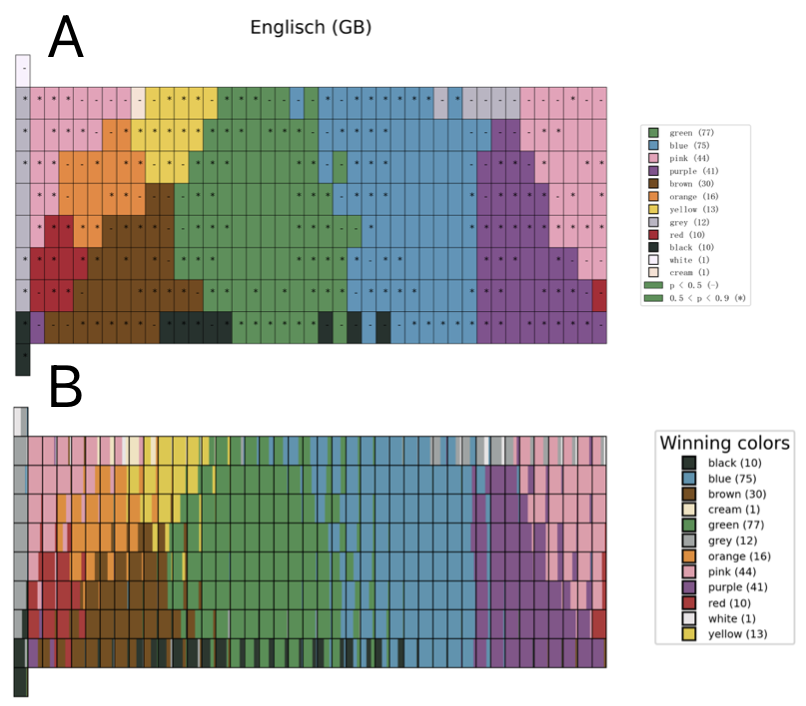
\includegraphics[width=\textwidth]{images/GradientAndMode.png}
%     \caption{Both show the same data we collected for English. A: Mode Map, B: \textit{NAME} map.
%     Mode maps give an overconfident impression about the solidness of  categories and hide much of information between.
%     }
%     \label{fig:maps}
% \end{figure}

\begin{figure}[htbp]
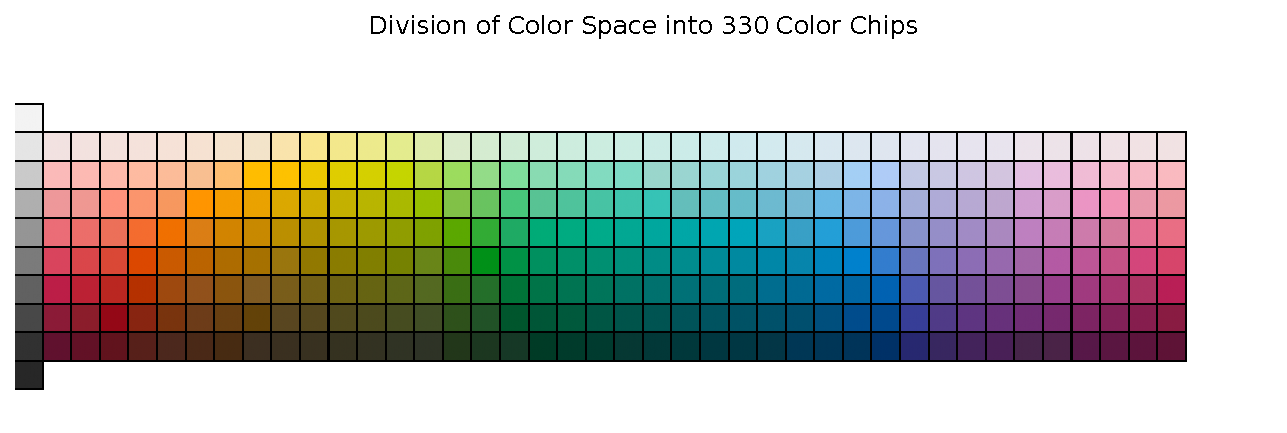
\includegraphics[page=1, width=0.88\linewidth]{images/munsell_chips.pdf}
% 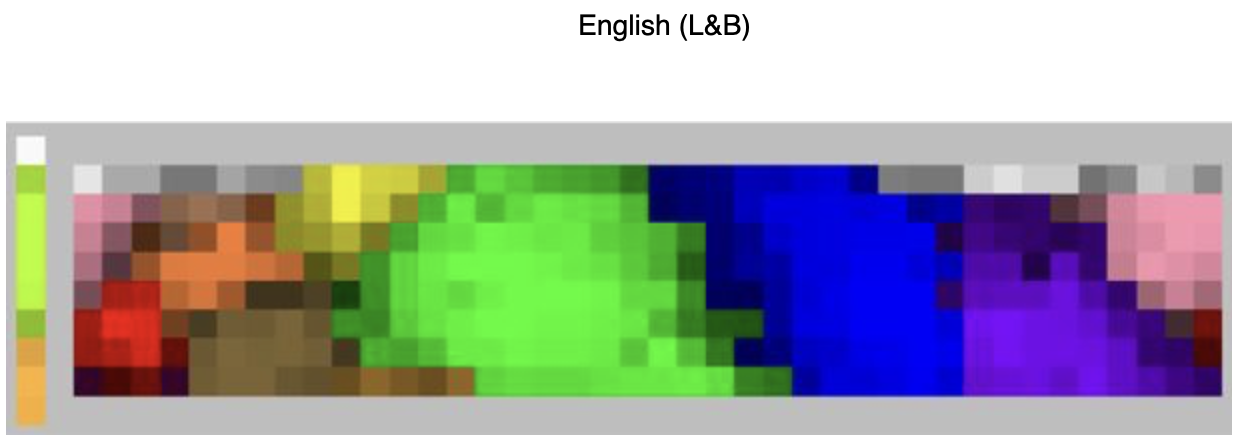
\includegraphics[page=1, width=0.81\linewidth]{images/LnB_generic.png}
% 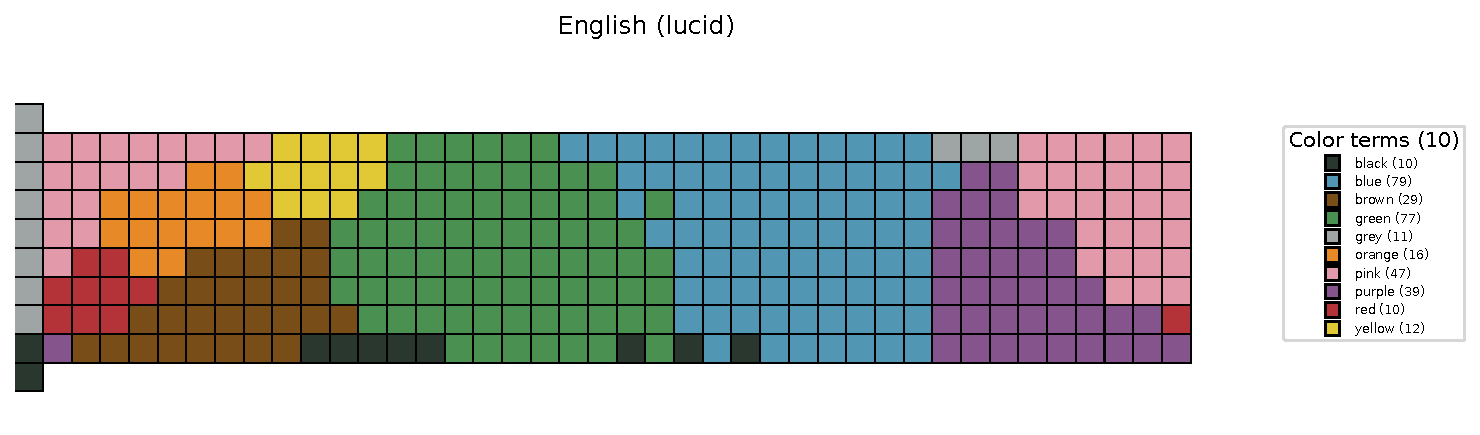
\includegraphics[page=1, width=\linewidth]{images/mode_maps/English (lucid)mode-map.pdf}
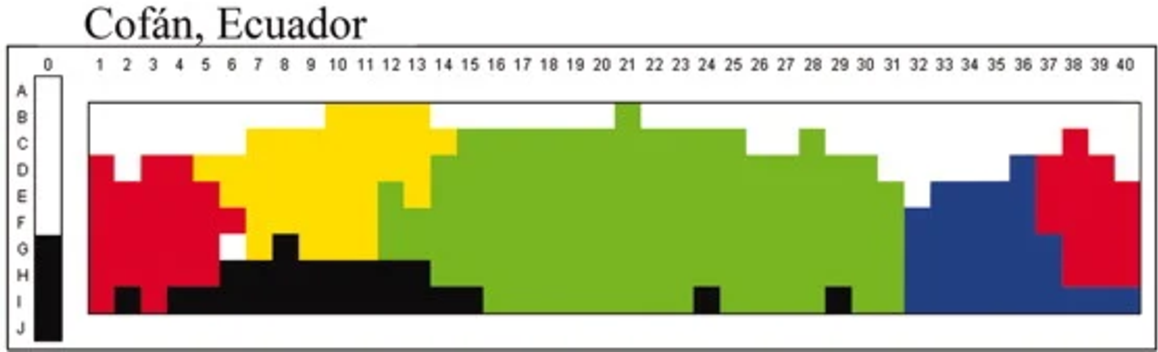
\includegraphics[page=1, width=0.81\linewidth]{images/mode_map.pdf}
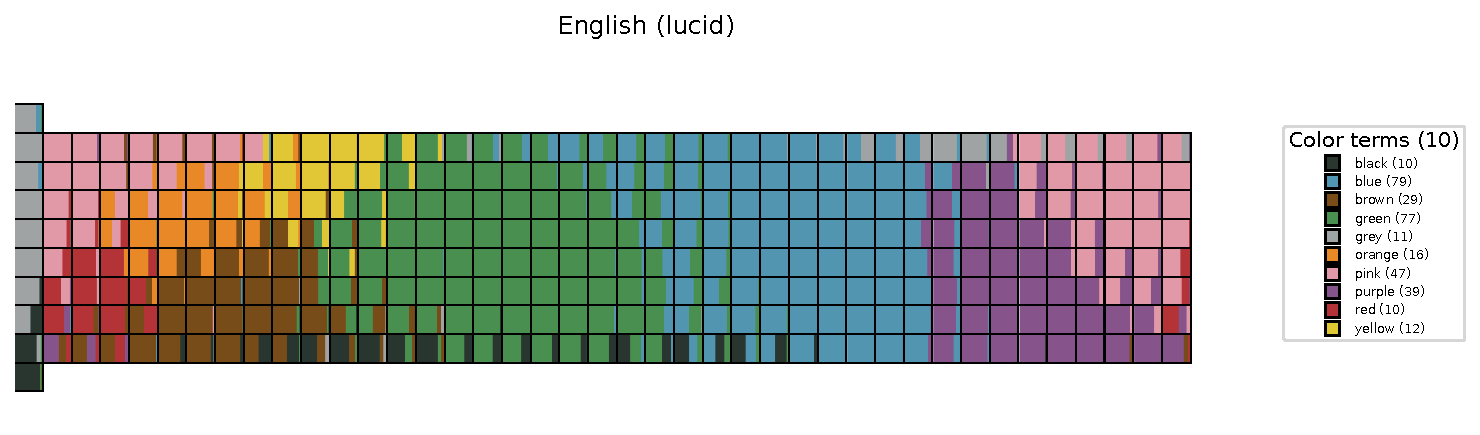
\includegraphics[page=1, width=\linewidth]{images/mode_maps/English (lucid).pdf}
\decoRule
\caption[330 Color Stimuli, Mode Map Regier et al. and Proportion Map]{330 Color Stimuli, Mode Map \parencite{regierColor2007} and Proportion Map. Upper panel: Subdivided color space into 330 color chips analog to the Munsell chips used in the WCS. Middle panel: Mode map of Cofán (Ecuador), a language examined in the WCS. Color naming pattern of six color categories visualized by \textcite{regierColor2007} using generic colors.
Lower panel: Proportional map using the mean RGB values for each color category. For each chip three most common color terms presented, therefore give intuitive information about the consensus for single color chips.}
\label{fig:mode_prop_maps}
\end{figure}
\section{Data-Analysis}

\subsection{Adjusted Rand Index}
To detect differences in color naming patters between the tested languages we used the adjusted rand index (ARI).
For every language we calculated the majority vote for all 330 color chips and transferred this naming pattern into a vector containing numeric representation of the winning color terms. This vector was then used to compute the ARI for each pair of languages using the scikit-learn implementation of the ARI \footnote{\url{https://scikit-learn.org/stable/modules/generated/sklearn.metrics.adjusted_rand_score.html}}. 

The ARI determines the similarity across cluster patterns which has been proven to be a reliable measure \parencite{rand1971objective}. It is adjusted for chance and takes a value between -1 and 1. A value of 1 indicates a perfect agreement between the two clusterings, whereas a value of 0 indicates a low expected similarity between two random clusterings \parencite{Hubert1985}. The resulting ARI matrix provides information about the similarity and dissimilarities between naming patterns of tested languages.


\subsection{Multidimensional Scaling}
We used multidimensional scaling (MDS) to project the ARI-matrix into a 2D space and therefore gather information about similarities and dissimilarities across languages as geometrical representation \parencite{carroll1998multidimensional}.
To do so we used the \textit{scikit-learn }implementation \footnote{\url{https://scikit-learn.org/stable/modules/generated/sklearn.manifold.MDS.html}}.
This implementation requires a dissimilarity matrix as an input. Thus we first had to convert the similarity matrix obtained from the ARI calculation into a dissimilarity matrix.


\begin{itemize}
    \item $S$ is the similarity matrix based on the Rand Index.
    \item $D$ is the dissimilarity matrix.
\end{itemize}

\[
D = 1 - S
\]

% ARI was used in previous color works (e.g. \cite{lindseyColor2014})
% This approach appeared to be very sensitive to minor differences.
% Especially near the boundaries between categories, the belonging of single chips is not very stable.
% Therefore, the resulting MDS plot appeared not to be very informative.

% In our second alignment approach, we aimed to be more robust against these minor differences.
% After identifying the winning color term for each chip, we calculated the mean color chip for each color term.
% \todo{not sure if first tranlated into CIE lab space?}
% To compare languages, we then calculated the Euclidean distance between each color term in both languages.
% We assumed that the color terms with the smallest distance between them are the categories that are most similar.
% As a measure of similarity, we summed up all these distances \todo{Thats all??}
% This distance matrix was then again projected into a 2D space using MDS\@.
% By taking the means of each category, this analysis is more robust against minor differences in the color naming pattern.
% It, therefore provides a more stable and informative MDS.

\subsection{Entropy}
Entropy in our case describes the uniformness of the participants answers. In Information theory entropy measures the uncertainty or unpredictability of information content. It quantifies the average amount of information produced by a stochastic source of data. High entropy means the information has high variability and is less predictable, while low entropy indicates a more predictable source of information.

In our analysis, we compute the Shannon entropy, denoted as $H$, for a single color chip. This variable's entropy is calculated based on the probability distribution of each observed color term, denoted as $p_1, p_2, \ldots, p_n$, according to the formula:

\begin{equation}
H = -\sum_{i=1}^{n} p_i \log_2 p_i
\end{equation}

Here, $p_i$ signifies the probability of the occurrence of the $i$-th color term within the distribution. The base 2 logarithm implies that entropy is quantified in bits, reflecting the information content or uncertainty associated with the color terms' distribution.
The exponent of the entropy can also count the number of possible states or configurations. Therefore, the exponent of the global entropy of a language is an estimate of the number of color terms available for this language. In Figure \ref{fig:entropy_plot} the exponent of the global entropy (number of color terms in the respective language) is plotted against the exponent of the local entropy (mean consensus on single chips).

\subsection{Levenstein distance}
The Levenstein distance, also known as edit distance, calculates how many single-character-edits (deletions, insertions, substitutions) have to be done to change one word in an other. For example the edit distance between 'grue' and 'blue' equals 2.
During data cleaning we made use of "thefuzz"\footnote{\url{https://github.com/seatgeek/thefuzz}} a python packages that uses this calculation to create a measure of similarity between words.

\subsection{K-means clustering}
K-means clustering is an algorithm to subdivide data into k clusters optimized by a measure of distance. The calculations follows these steps: First, k cluster centers are initialized at random values. Second, all data points get assigned to the closest cluster center mostly using the euclidean distance. Third, new location of the cluster center is calculated by taking the mean of each cluster. Steps two and three get repeated until the assignments do not change anymore or the change is below a certain threshold. We used this method to find distinct clusters in the naming patterns of the human data.


\subsection{Color Term Frequency}
"wordfreq" \footnote{\url{https://github.com/rspeer/wordfreq}} is a python library that enables to look up the frequency of usage of words in a specified language based on a large dataset. This was used in the cleaning procedure to detect typos. All color terms of a score = 0 were considered to be possible typos.
Furthermore, in Fig. \ref{fig:frequency_plot} we investigated the color term frequency found for GPT4 and human data to determine which one uses less frequent terms for the respective language.
\section{Experimental hypothesis}

\begin{itemize}
    \item This research project is the first to use Lucid Marketplace to recruit participants. Lucid promises many advantages such as a vast quantity of participants of up to 112 countries and 73 languages. However, the data quality has yet to be tested and controlled using control experiments on traditional recruiters that have been tested extensively during earlier research.
    Therefore, we launched the same experiment in four different languages, Greek, English, Italian and Russian analog on Prolific and Lucid. Comparison of these four dataset are expected to result in high accordance and similarity.
    \item We identified the data of \textcite{lindseyColor2014} to be a good reference and control group for an in-lab conducted experiment. Because of the difficulties related to online experiments we need to compare our results to an in-lab experiment that used the same or comparable procedure conditions to verify the quality of the collected data.
    \item \textcite{kayWorld2009} suspected globalization effect to erase cross linguist distinctions in color terminology. However, other studies have proven the stabilization of new BCT in different languages. Therefore, we expect to find updated color vocabularies containing newly emerging color terms for each specific language.
    \item A lot of research has been done to detect universal rules in how the categories are located in color space. Color naming pattern have been proven to be determined a.o. by the irregularities of color space and principles of categorization and the rules of information theory. 
    For the newly emerging color categories we expect to detect similar universal developments.
    \item GPT4 is a LLM trained on massive text corpora enabling the model to produce text about colors. Because GPT4 derives its information about colors solely out of these text sources, we expect language-specific color naming patterns to be preserved in the data. However, GPT4 is trained on multiple languages and therefore contains information about different color naming patterns. We will try to observe these cross lingual influences.
\end{itemize}


\chapter{Results}
% \section{Participants}

We collected data from 25 groups (21 in Lucid and 4 in Prolific, with 22 unique languages across both recruiters).
We recruited between 40 and 229 participants per group (mean: 91.2, sd: 41.7). 
Altogether, we collected data from 2,280 participants (Lucid: 1,763, Prolific: 517). 
The mean age across all participants was 42 (sd: 15)
%and 31% of the participants have at least a Bachelor’s degree.


We indeed see a relatively high mean age of the participants
we also see diverse levels of education ranging from non to graduate or higher. 
also the relevant education in colors has a great range

\section{Human Data}
\subsection{Data Quality}

Visualization in mode-maps gives qualitative confirmation that the data and the cleaning procedure give reasonable information about the color lexicon of the respective languages (Fig. \ref{fig:color_maps_english}).
Overall, we found the split-half ARI value for all languages to be high (range=.66-.88, mean=.75 sd=.05, Tabl.: \ref{tab:pgfplotstable_csv}).


\subsection{Comparison between Recruiters}

 Figure \ref{fig:color_maps_english} shows the English proportional maps obtained from Prolific and Lucid and compares them to the maps by \textcite{lindseyColor2014} (data reproduced with permission). 
We found a high ARI between \textcite{lindseyColor2014} and Prolific and Lucid (.72 [.67, .77] and .67 [.62, .72], respectively, CIs via bootstrapping, Fig. \ref{fig:color_maps_english}). 
For other languages that were tested on both recruiters (English, Italian, and Greek), the ARIs were also high (.70 [.65, .74], .61 [.56, .66], and .63 [.57, .68], respectively, (Fig. \ref{fig:color_maps_english}). 

 % In these maps, each chip is colored by the majority vote for this particular chip. We plot the color of the region associated with a term to be the average color (in RGB space) across all winning chips. 
 As indicated by the legends, participants mention similar color categories which cover similar proportion of chips across the data sets.
 The prolific sample includes two newly emerging color terms 'lilac' and 'teal' which are already discussed by \textcite{lindseyColor2014}.
 Majority vote over all participants on Lucid converged on the 11 basic color categories proposed by \textcite{berlinBasic1969} with white as one exception.
 Interestingly, throughout our dataset we see a consistently small or utterly absent white category. This is most likely due to the way we present the stimulus (Fig. \ref{fig:col-trail}). The square of color is presented on a white page. When showing very light chips a side effect might be that they never meet exactly the white of the page right next to the stimulus. The task undeliberately turns into a distinction task which makes it easy for people to see the very light color instead of just white.

 

\begin{figure*}[h!t]
    \begin{center}    
    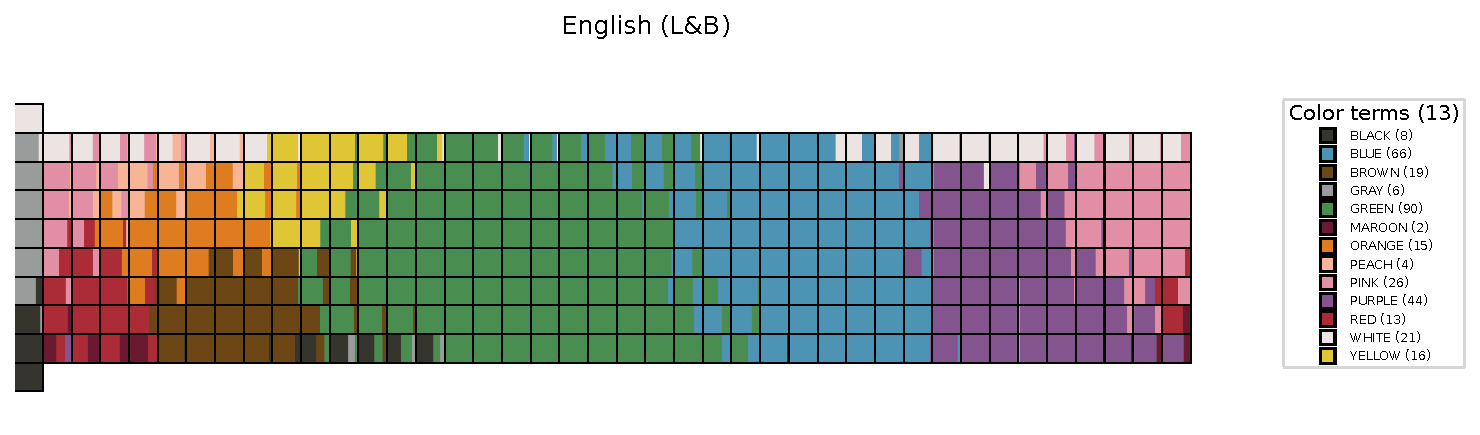
\includegraphics[page=1, width=\linewidth]{images/mode_maps/English (L&B).pdf}
    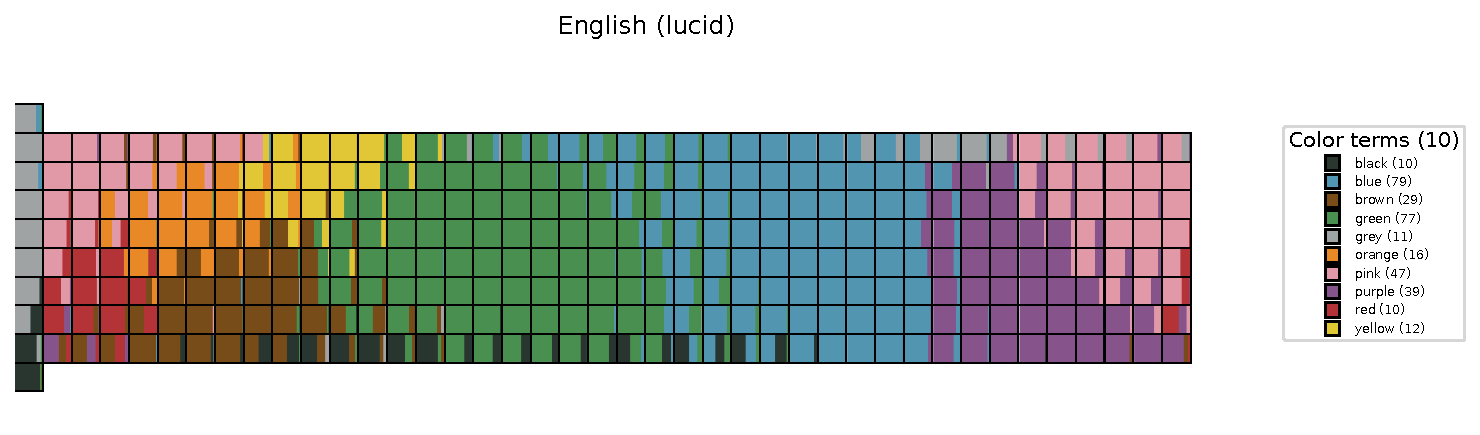
\includegraphics[page=1, width=\linewidth]{images/mode_maps/English (lucid).pdf}
    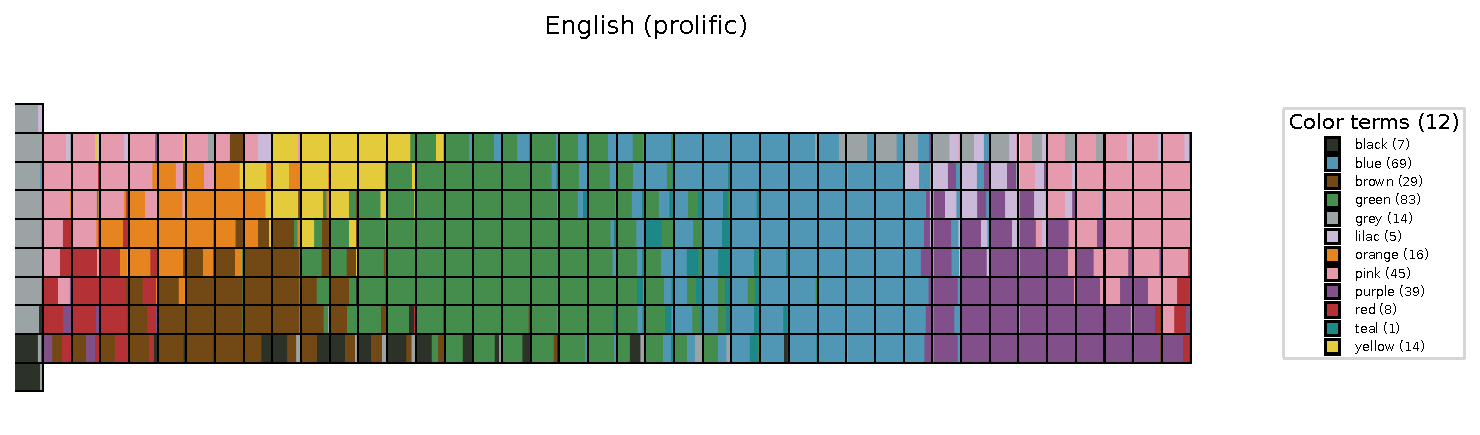
\includegraphics[page=1, width=\linewidth]{images/mode_maps/English (prolific).pdf}
    \end{center}
    \caption[English Proportional maps]{English Proportional maps: Upper panel: Reproduction of data from an in lab experiment by \textcite{lindseyColor2014} with permission. Middle and lower panel: Newly online collected Data on different recruiters Prolific and Lucid.
    Proportional maps show qualitatively high accordance across the different occasions of data collection.}
    \label{fig:color_maps_english}
\end{figure*}

\begin{figure*}[h!t]
    \begin{center}    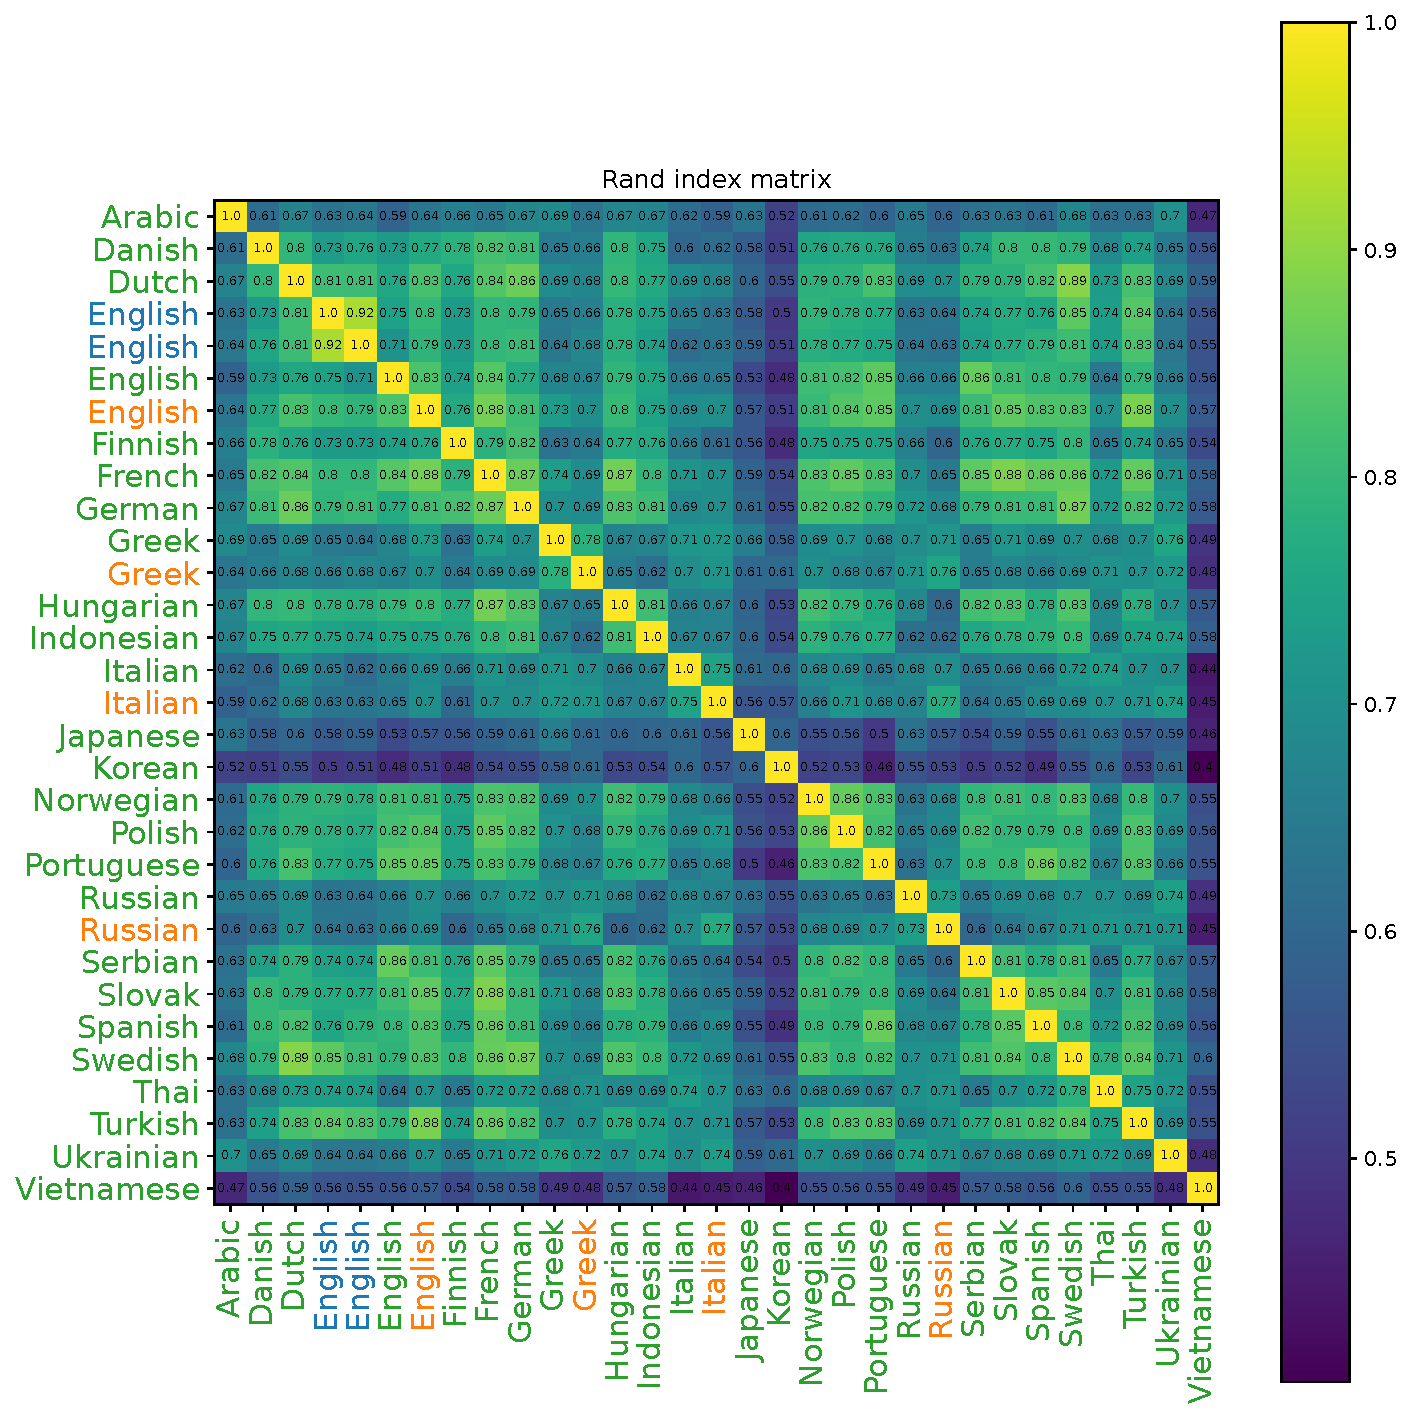
\includegraphics[width=\textwidth,height=\textheight,keepaspectratio]{images/rand_index_matrix_all.pdf}
    \end{center}
    \decoRule
    \caption[Rand Index Matrix human data]{Rand Index Matrix for human data from \textcite{lindseyColor2014} (blue) and newly collected data on recruiters Prolific (orange) and Lucid (green). Rand index indicates similarity of naming pattern of respective languages, ranging from 1, exactly the same, to 0, dissimilar clustering.}
    \label{fig:rand_index_matrix}
\end{figure*}


\subsection{Comparing to WCS Data}

% Mean ARI (Uniformness of the dataset)
Compared to the WCS languages the collected dataset seem more homogeneous.
The mean ARI across the entire dataset is .70 [.50, .89] whereas it is much lower across the WCS languages (.43 [.18, .68]).
Across both data sets, the mean ARI is significantly lower .31 [.05, .57] than within the two data sets (p<.001 for both cases via the Mann-Whitney U test), confirming the difference.
% Number of Color Term
Significant distinction was also found for the number of color terms which was higher in the Lucid dataset (9.02 [5.92, 12.12]) than for the WCS data (5.71 [2.57, 8.85], p<.001 via the Mann-Whitney U test).
The number of color terms here is calculated by computing the exponent of the entropy on all chips.
The variance of the number of color terms was equally high in both data sets.


\subsection{Analysis of Single languages}

\paragraph{English:}
\textcite{berlinBasic1969} claimed to have found eleven basic color categories represented by the 11 English color categories \textit{black, white, red, yellow, green, blue, brown, orange, pink, purple, and gray}.
The English data elicited on Lucid reproduced this list of color terms with one exception: white.
Because of the high concordance with the literature the English data will be used as a reference when analysing other languages.
(Split-half-rand-index = 0.85)

\paragraph{Arabic:}

We found a relatively broad lexicon for Arabic, namely 18 winning color terms. Interestingly, there is a distinction in the blue category differentiating \textit{light blue} from \textit{dark blue}.
Furthermore, many color terms are derived from objects such as the word for \textit{grey}
\begin{Arabic}رمادي\end{Arabic}(ramadi), coming from \begin{Arabic}رماديرماد\end{Arabic}(ramad), which means ashes or \begin{Arabic}رصاصي\end{Arabic}(rṣaṣi) translates to lead.
The data show a relatively large white category of six chips. (Split-half-rand-index = 0.66)


\paragraph{Danish:}
% hvid} (2)
Aligns to the English color lexicon covering all BCT.
Interestingly, we see a \textit{white} category of only small size covering two color chips.
(Split-half-rand-index = 0.74)

\paragraph{Dutch:}
The dutch color lexicon contains apart from \textit{white} all eleven BCT plus one additional small \textit{lila} category and a double category for \textit{roze} which was not caught by our cleaning algorithm.
Here the \textit{white} category is entirely absent. 
(Split-half-rand-index = 0.76)

\paragraph{Finish:}
Finish data show all BCT plus a \textit{lila} and \textit{turkoosi} category.
Here the \textit{white} category wins in 3 chips.
(Split-half-rand-index = 0.73)

\paragraph{French:}
French data show high accordance with the BCT. However the white category only covers 1 chip.
(Split-half-rand-index = 0.81)

\paragraph{German:}
In addition to the BCT which are all present in the German data ocker \textit{türkis} and \textit{beige} are introduced as additional color terms.
(Split-half-rand-index = 0.79)

\paragraph{Greek:}
Greeks belong to the languages differentiating between \textit{light blue} \textgreek{θαλασι} (thalassi) sea and \textit{dark blue} \textgreek{μπλε} (ble).
%\textgreek{λάχανο} (lachano) literally translates to cabbage and might have been used metaphorically for a color, but it's not a standard color term in Greek.
\textgreek{κιτρινοπο} seems to be a spelling which was conserved despite our cleaning procedure and represents the standard word for \textit{yellow} \textgreek{κίτρινο} (kitrino).
\textgreek{τιρκοθαζ} is the direct translation of \textit{turquise} into Greek letters but is not considered to be a native Greek word.
(Split-half-rand-index = 0.77)

\paragraph{Hungarian:}
The elicited color lexicon for Hungarian covers all BCT.
In addition we found a quite large category \textit{bordo} for \textit{dark-red}.
(Split-half-rand-index = 0.75)

\paragraph{Indonesian:}
The Indonesian color lexicon includes all BCT plus one small category krem.
A small \textit{white} category is present as well.
(Split-half-rand-index = 0.76)

\paragraph{Italian:}
Italian belongs to the list of languages making distinctions between \textit{blu} - \textit{blue} and \textit{azzurro }- \textit{light blue}. Interestingly, Italian possesses one additional category for blue: \textit{celeste} which means\textit{ very} \textit{light blue}.
\textit{Verdino} also shows up in the list which means \textit{greenish} but did not get caught by the cleaning procedure.
(Split-half-rand-index = 0.74)

\paragraph{Japanese:}
Japanese makes three distinctions in the blue category.
First, \japaneseText{アオ色} (ao-iro): basic \textit{blue} color. Second, \japaneseText{コン色} (kon-iro): \textit{navy blue} or \textit{deep blue} color. Third, \japaneseText{ミズ色} (mizu-iro): Water color, often referring to a clear, \textit{light blue}.
\japaneseText{ダイダイ色} (daidai-iro) represents a specific type of \textit{orange} color. Daidai refers to a specific shade of \textit{orange}, named after the bitter orange fruit.
\japaneseText{モモ色} (momo-iro) means \textit{peach}, \japaneseText{ハダ色} (hada-iro) \textit{skin color} and \japaneseText{ヒ色} (hi-iro) which is likely a typo or shorthand. If it meant to be \japaneseText{ヒワ色} (hiwa-iro), it would refer to a \textit{light yellow}.
All other color terms refer to the BCT named by Berlin and Kay with only white missing.
The relatively large color lexicon that we found is consistent with earlier studies that claimed to have found 16 statistically distinct color terms for Japanese \parencite{kurikiModern2017}.
(Split-half-rand-index = 0.73)

\paragraph{Korean:}
Korean possesses a very large color term lexicon. Interesting distinctions here are between \textkorean{파란색} (paransaek) - \textit{Blue} and 
\textkorean{하늘색} (haneulsaek) - \textit{Sky Blue}. 
Green is subdivided by three terms: 
\textkorean{녹색} (noksaek) Green
\textkorean{연두색} (yeondusaek) light green or lime green and
\textkorean{초록색} (choroksaek) another term for green, often used to describe nature.
The white category is missing.
(Split-half-rand-index = 0.47)


\paragraph{Norwegian:}
Norwegian color lexicon covers all BCT plus turkis and a double category for orange.
(Split-half-rand-index = 0.69)

\paragraph{Polish:}
All BCT present in the polish lexicon and two additional categories granatowy and bordowy. No white category here.
(Split-half-rand-index = 0.72)

\paragraph{Portuguese:}
Portuguese makes a profound distinction between lilás and roxo but does not report a white category.
(Split-half-rand-index = 0.81)

\paragraph{Russian:}
Most interestingly, Russian distinguishes between \textrussian{голубой} (goluboy) light blue or sky blue and \textrussian{синий} (siniy) which means blue.
Additional categories are: \textrussian{бордовый} (bordovyy): Burgundy and the distinction between \textrussian{сиреневый} (sirenevy): Lilac and \textrussian{фиолетовый} (fioletovyy): Purple
(Split-half-rand-index = 0.75)

\paragraph{Serbian:}
The serbian color lexicon coveres all BCT.
(Split-half-rand-index = 0.77)


\paragraph{Slovakian:}
Apart from the BCT slovakians inlude a small category for bordovy.
(Split-half-rand-index = 0.78)

\paragraph{Spanish:}
The data align very well to the english BCT but make a distinction between morado, lila and violeta in the purple region.
(Split-half-rand-index = 0.77)

\paragraph{Swedish:}
All BCT are covered by the Swedish lexicon plus one small category beige
(Split-half-rand-index = 0.74)

\paragraph{Thai:}
Contains all BCT apart from white, and makes distiction between \textthai{น้ำเงิน} (Nam ngern) blue and \textthai{ฟ้า} (Fa) sky blue or light blue.
(Split-half-rand-index = 0.76)

\paragraph{Turkish:}
Turkish basic color vocabulary covers all BCT with a very small white category and an additional small lila category.
Furthermore, it makes a distinction in the red area to dark-red bordo and dark blue lacivert.
(Split-half-rand-index = 0.74)

\paragraph{Ukrainian:}
We found a very comprehensive color vocabulary for Ukrainian with many small and specific categories.
Interesting however, is the large category for light-blue \textukrainian{блакитний} (blakytnyi) and light or lettuce and fresh green \textukrainian{салатовий} (salatovyi).
(Split-half-rand-index = 0.71)

\paragraph{Vietnamese:}
This is the only language we examined that does not cover all BCT. Vietnamese puts the green and blue category together in a grue category \textit{xanh}.
(Split-half-rand-index = 0.88)

% \paragraph{Summary:}
% Presence of a light blue category: Arabic, Greek, Italian, Japanese, Korean, Russian, Thai and Ukrainian.

% Presence of a blue category: Danish, Dutch, English, Finnish, French, German, Hungarian, Indonesian, Norwegian, Polish, Portuguese, Serbian, Slovakian, Spanish, Swedish, Turkish



\begin{figure}[htbp]
\centering
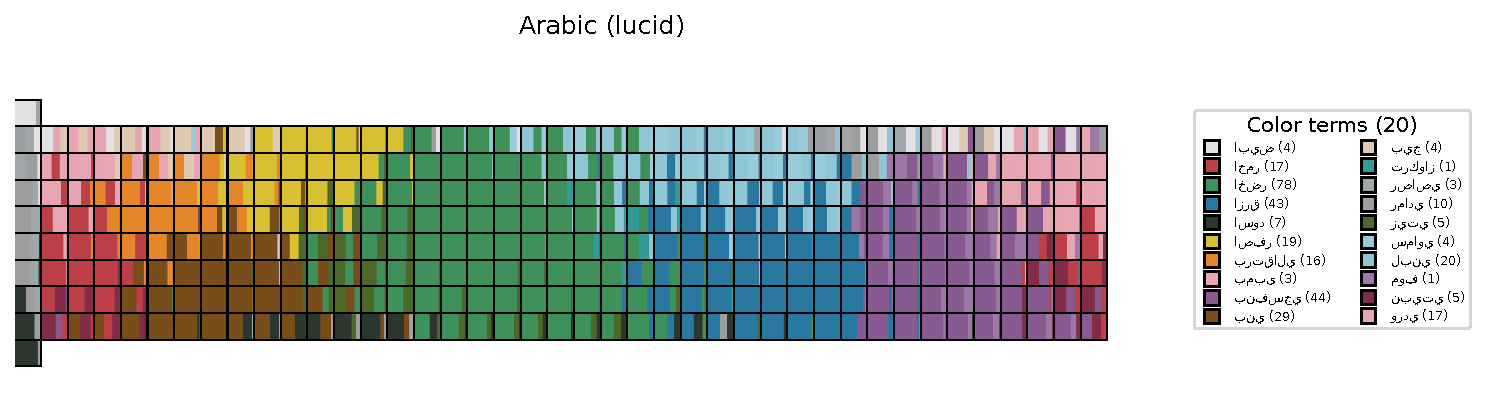
\includegraphics[page=1, width=\linewidth]{images/mode_maps/Arabic (lucid).pdf}
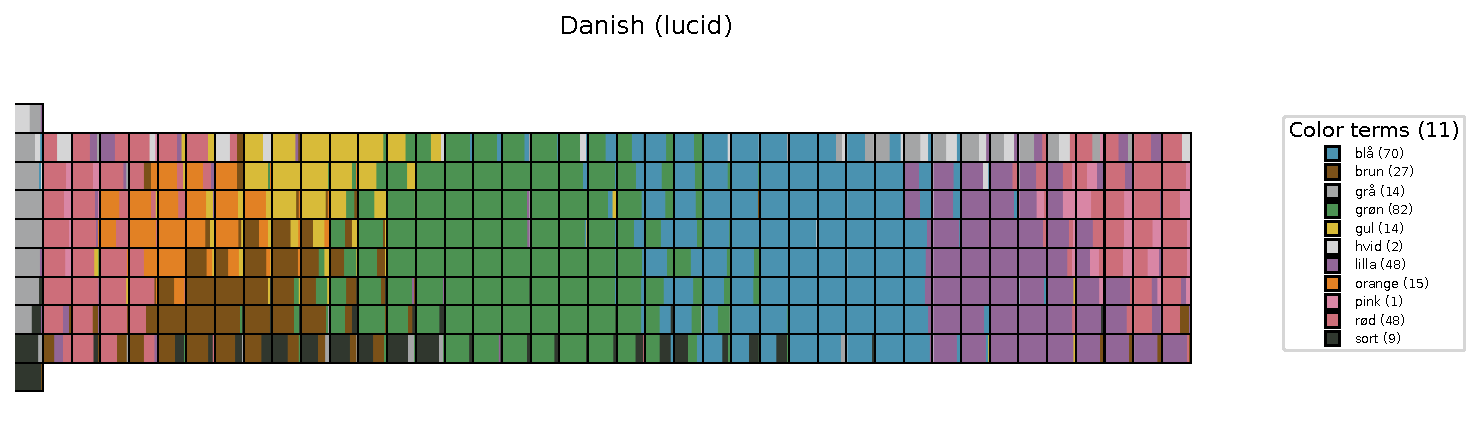
\includegraphics[page=1, width=\linewidth]{images/mode_maps/Danish (lucid).pdf}
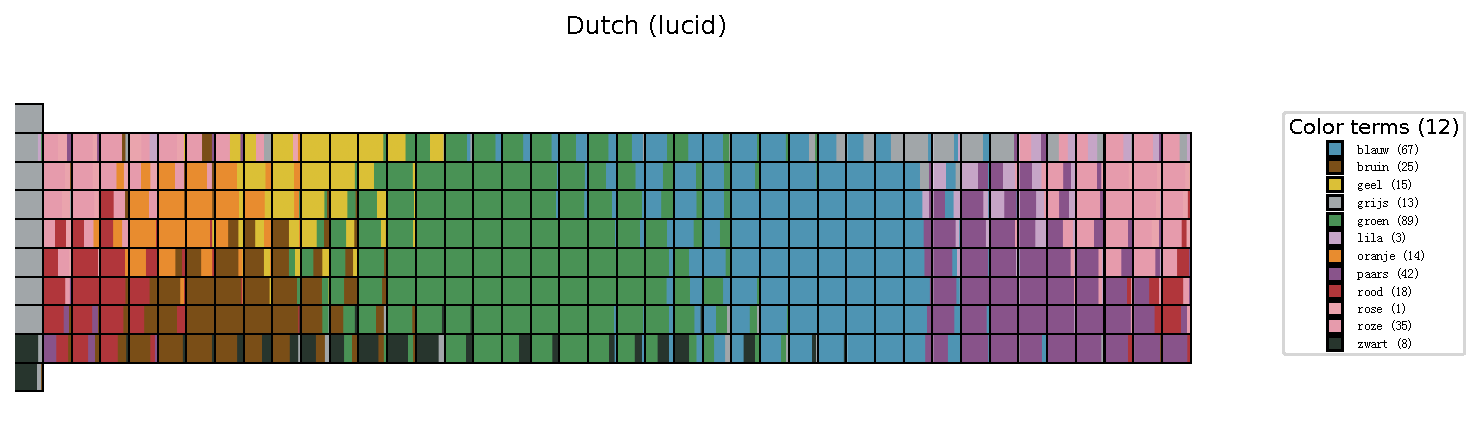
\includegraphics[page=1, width=\linewidth]{images/mode_maps/Dutch (lucid).pdf}
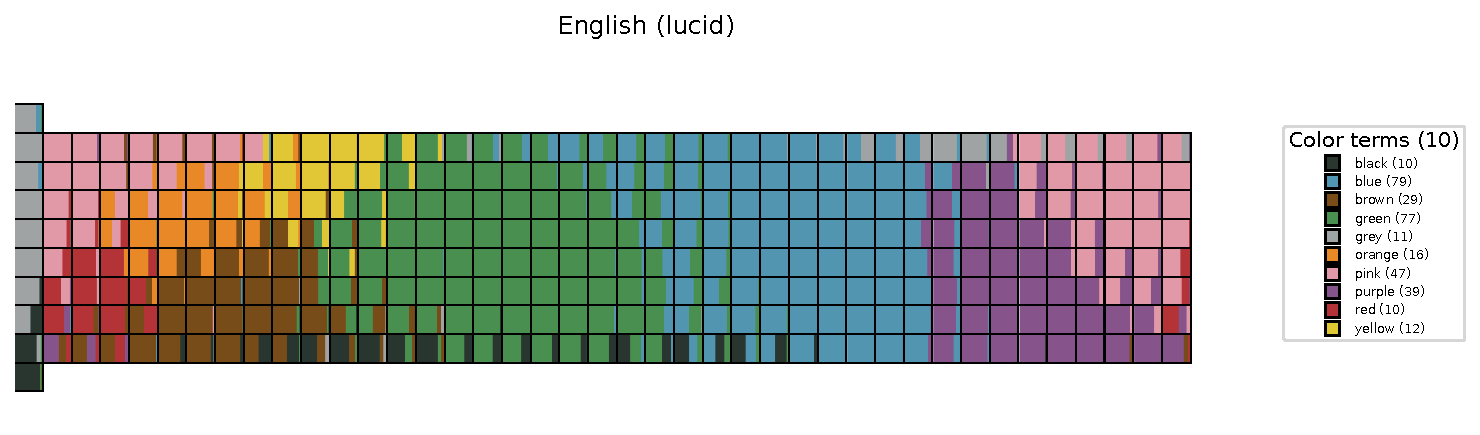
\includegraphics[page=1, width=\linewidth]{images/mode_maps/English (lucid).pdf}
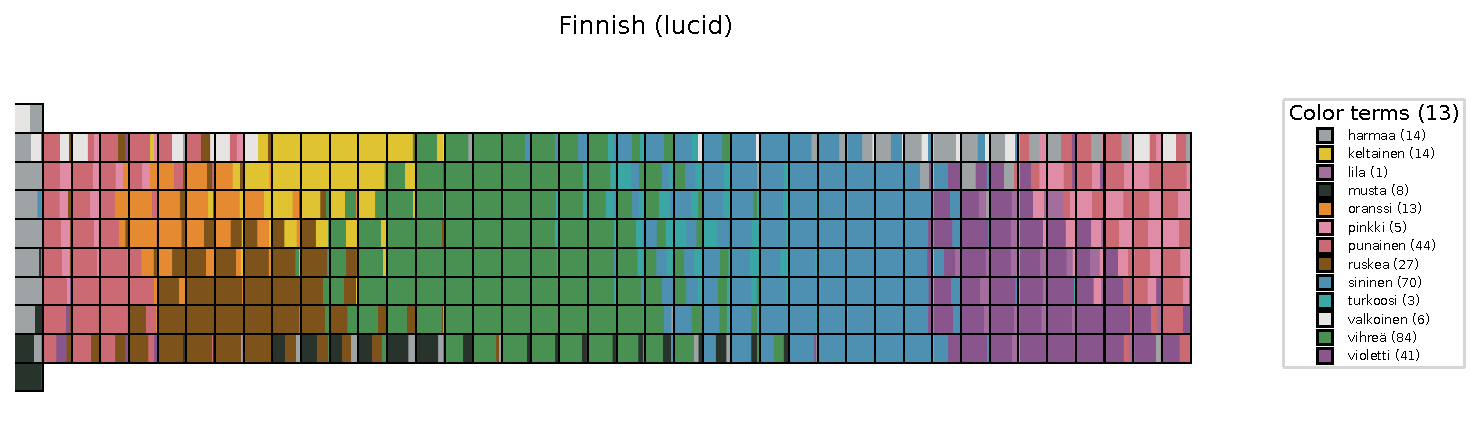
\includegraphics[page=1, width=\linewidth]{images/mode_maps/Finnish (lucid).pdf}
\caption[Proportion Maps (Arabic, Danish, Dutch, English, Finnish]{Proportion maps for Arabic, Danish, Dutch, English, Finnish and respective color terms.}
\label{fig:color_maps_1}
\end{figure}

\begin{figure}[htbp]
\centering
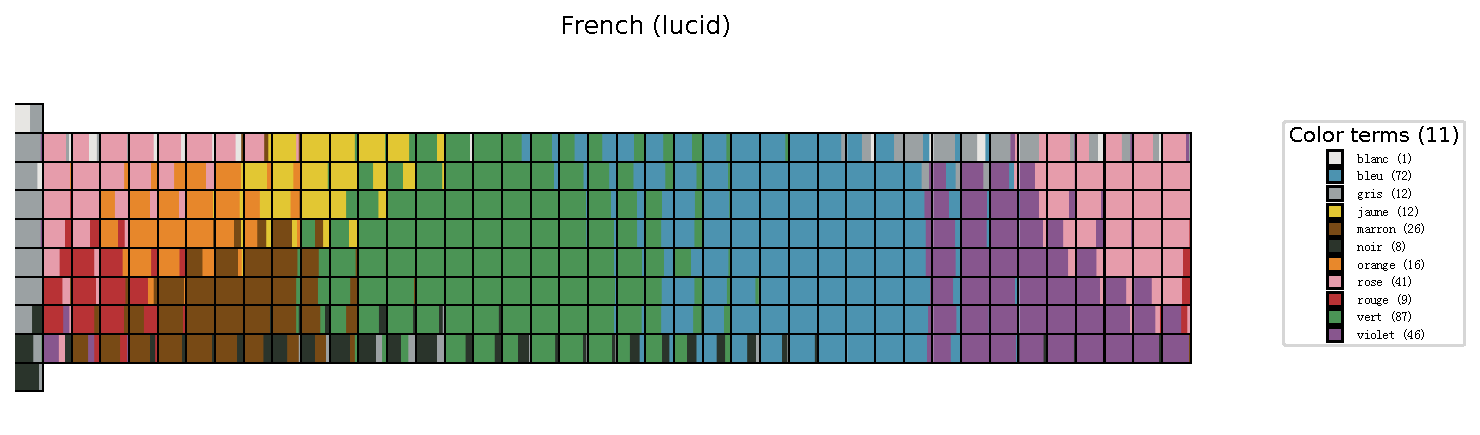
\includegraphics[page=1, width=\linewidth]{images/mode_maps/French (lucid).pdf}
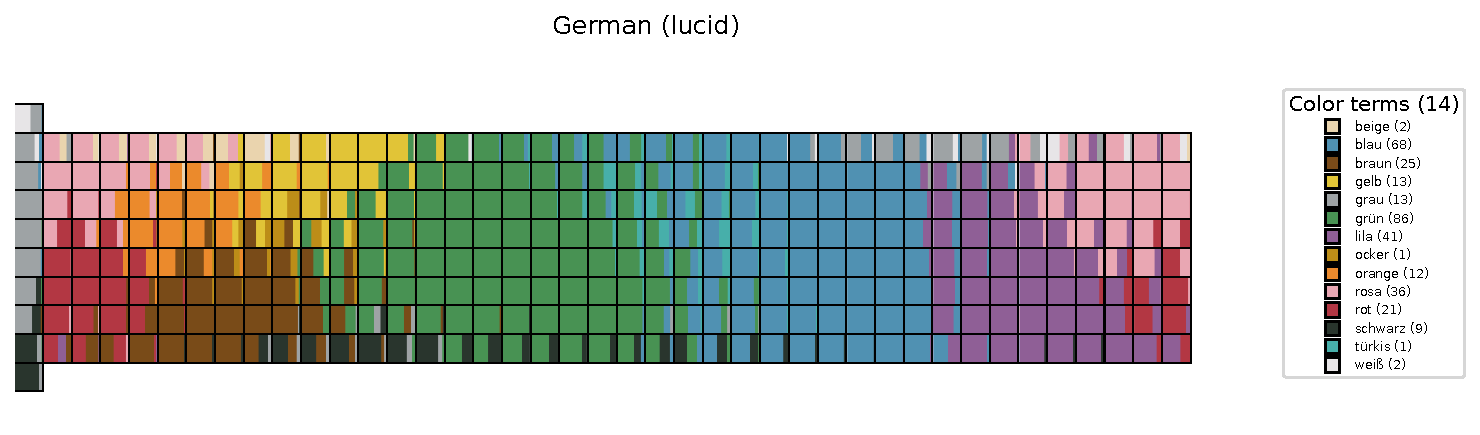
\includegraphics[page=1, width=\linewidth]{images/mode_maps/German (lucid).pdf}
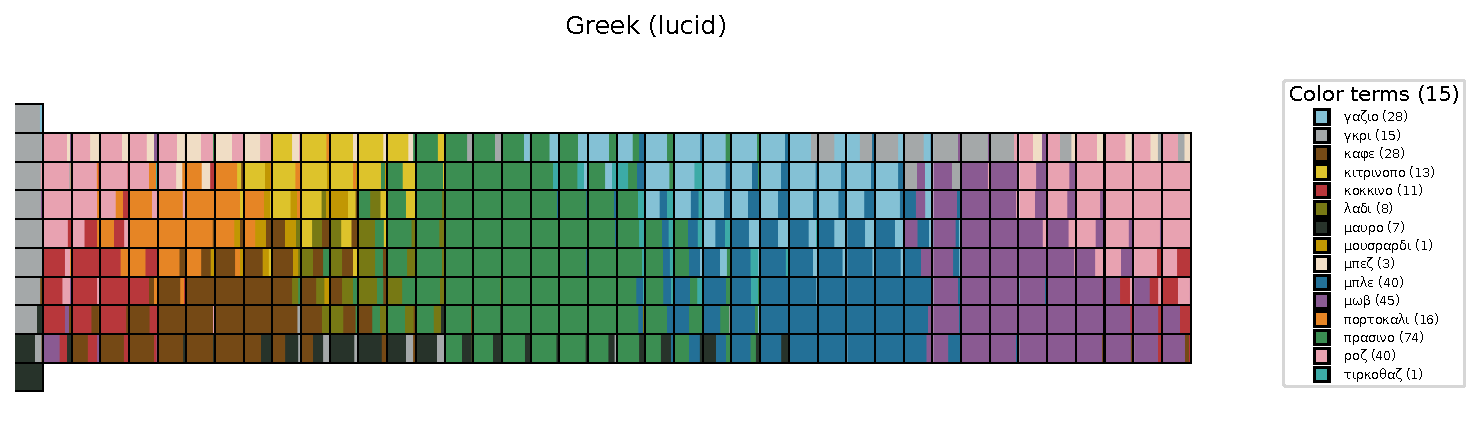
\includegraphics[page=1, width=\linewidth]{images/mode_maps/Greek (lucid).pdf}
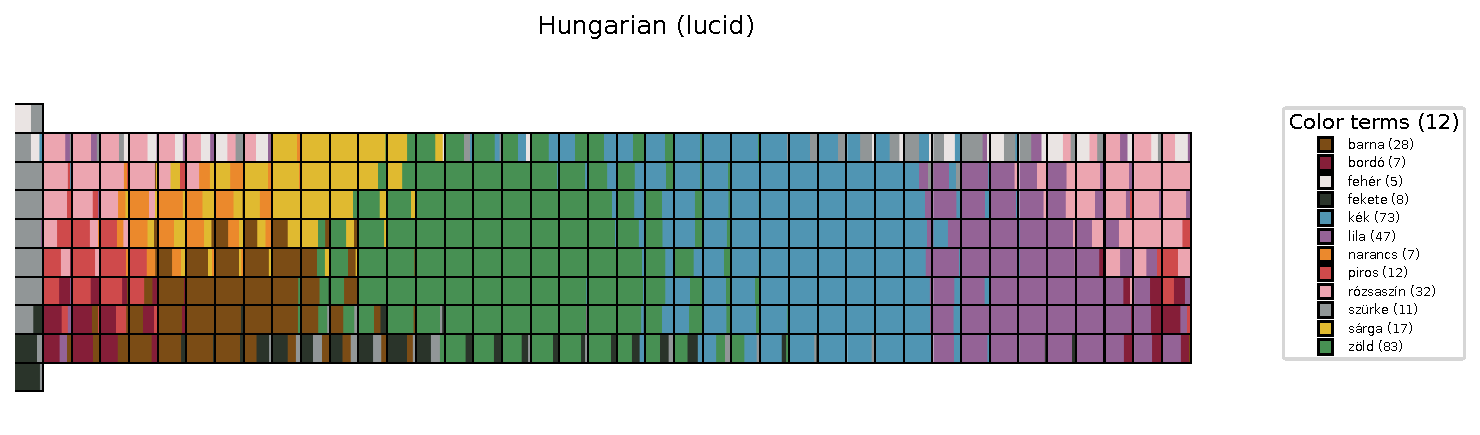
\includegraphics[page=1, width=\linewidth]{images/mode_maps/Hungarian (lucid).pdf}
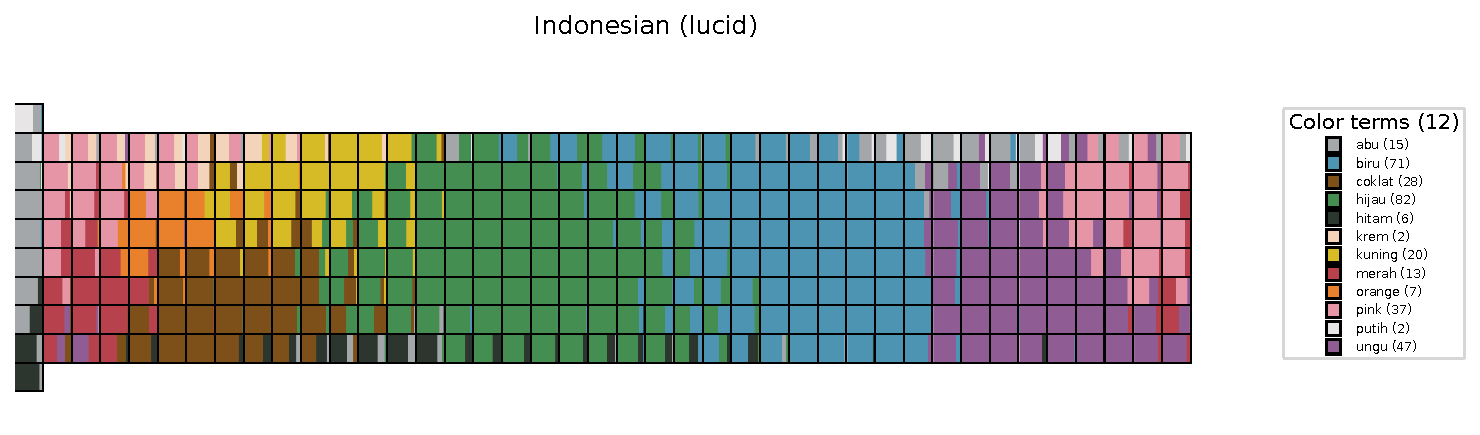
\includegraphics[page=1, width=\linewidth]{images/mode_maps/Indonesian (lucid).pdf}
\caption[Proportion Maps (French, German, Greek, Hungarian, Indonesian)]{Proportional maps for French, German, Greek, Hungarian, Indonesian and respective color terms.}
\label{fig:color_maps_2}
\end{figure}

\begin{figure}[htbp]
\centering
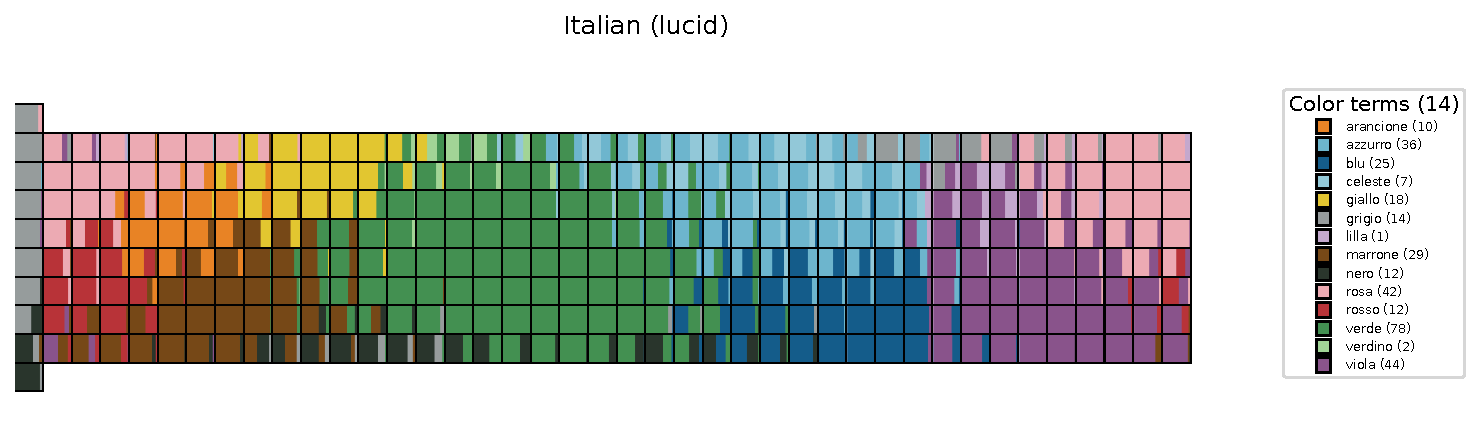
\includegraphics[page=1, width=\linewidth]{images/mode_maps/Italian (lucid).pdf}
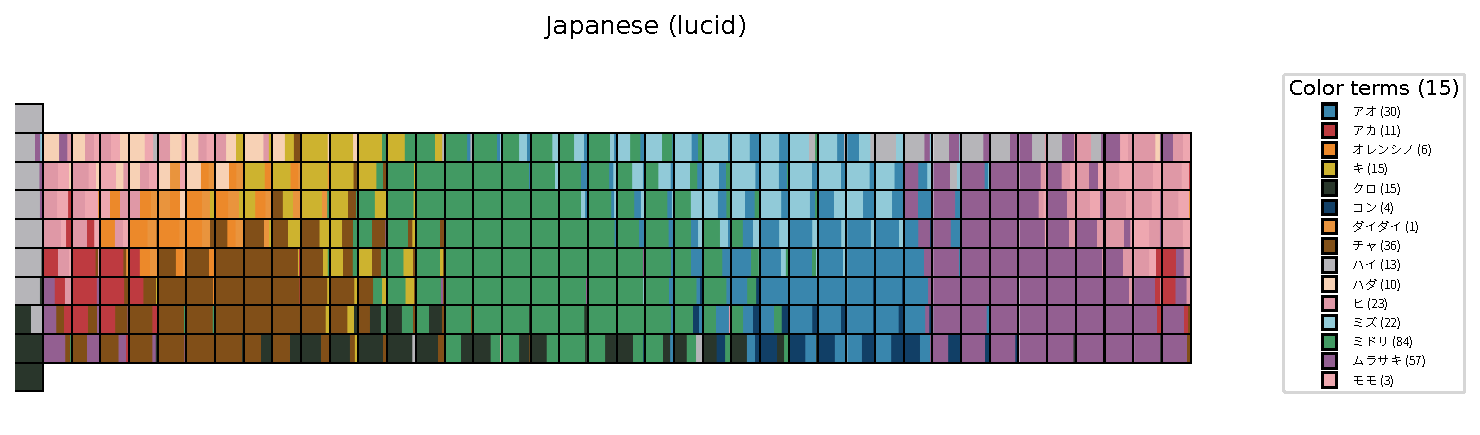
\includegraphics[page=1, width=\linewidth]{images/mode_maps/Japanese (lucid).pdf}
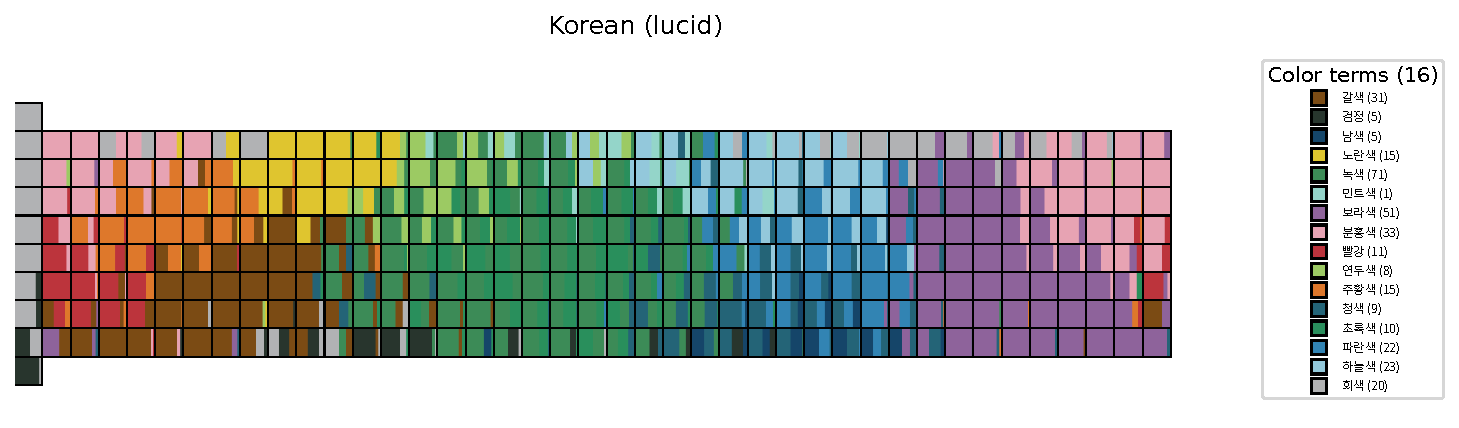
\includegraphics[page=1, width=\linewidth]{images/mode_maps/Korean (lucid).pdf}
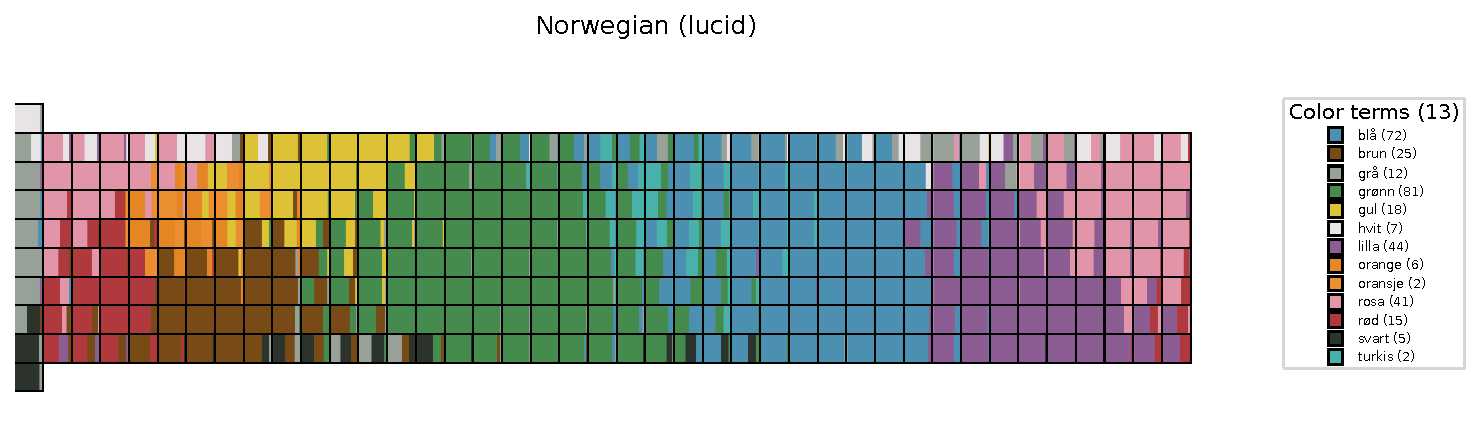
\includegraphics[page=1, width=\linewidth]{images/mode_maps/Norwegian (lucid).pdf}
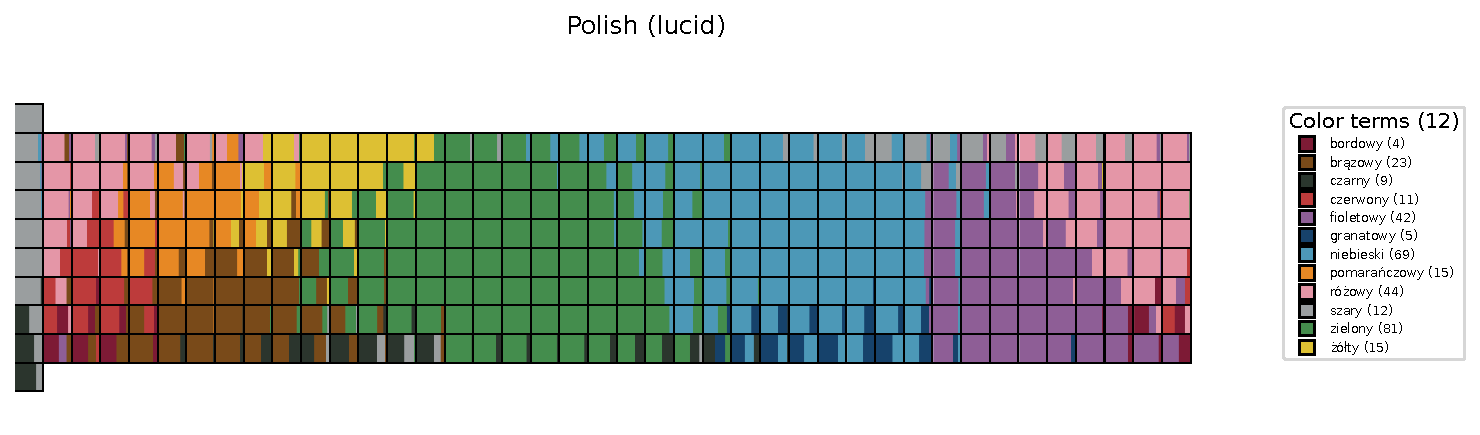
\includegraphics[page=1, width=\linewidth]{images/mode_maps/Polish (lucid).pdf}
\caption[Proportion Maps (Italian, Japanese, Korean, Norwegian, Polish)]{Proportional maps for Italian, Japanese, Korean, Norwegian, Polish and respective color terms.}
\label{fig:color_maps_3}
\end{figure}

\begin{figure}[htbp]
\centering
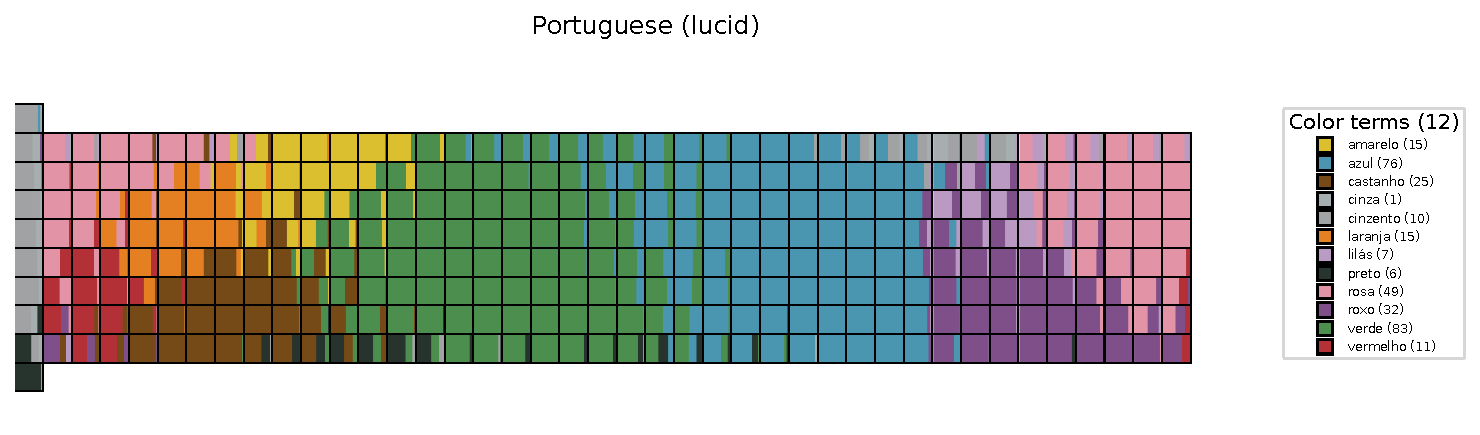
\includegraphics[page=1, width=\linewidth]{images/mode_maps/Portuguese (lucid).pdf}
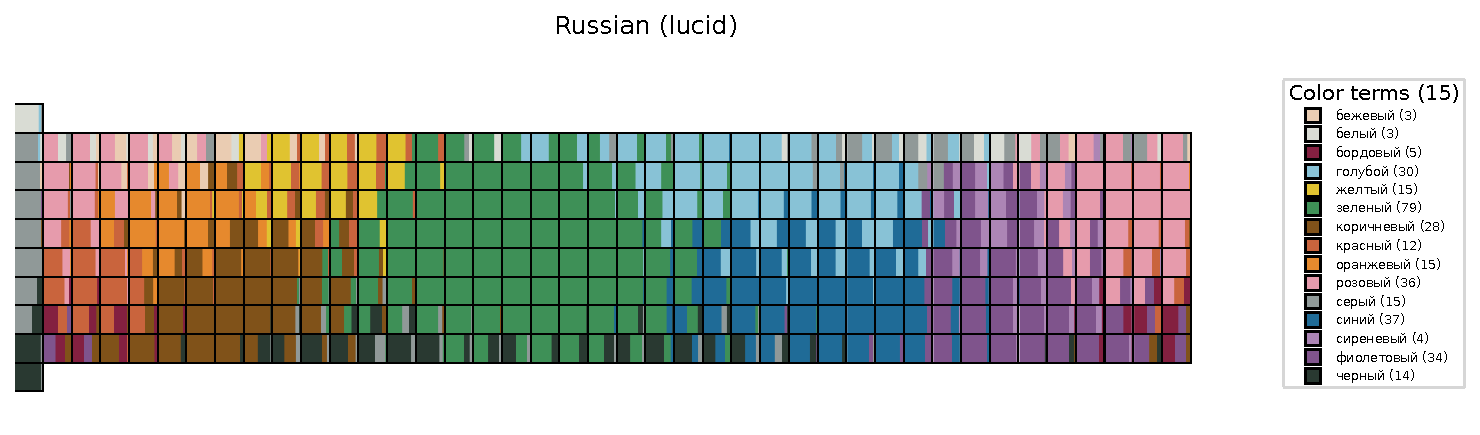
\includegraphics[page=1, width=\linewidth]{images/mode_maps/Russian (lucid).pdf}
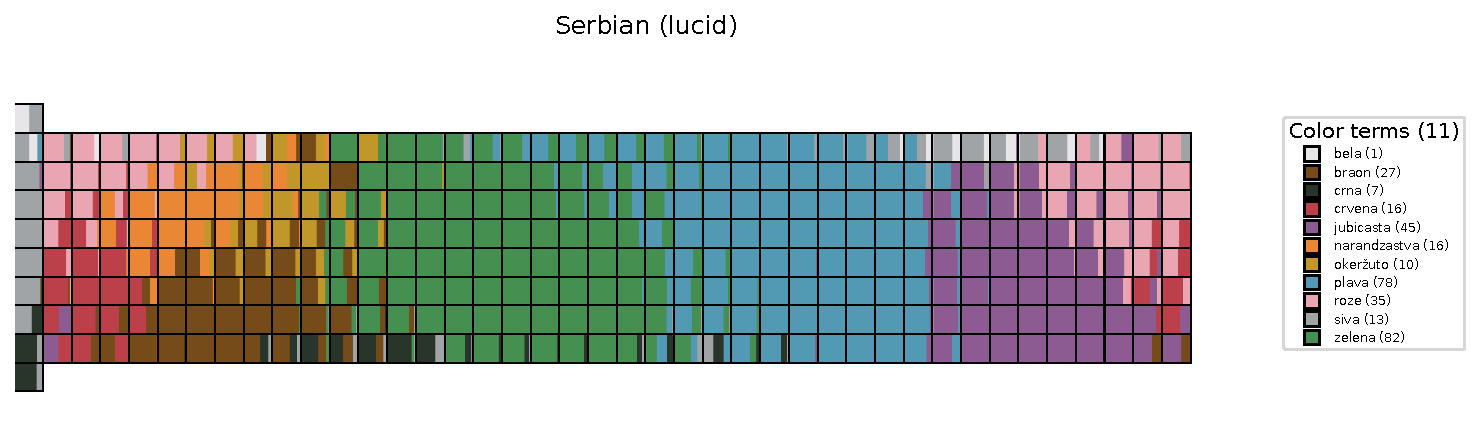
\includegraphics[page=1, width=\linewidth]{images/mode_maps/Serbian (lucid).pdf}
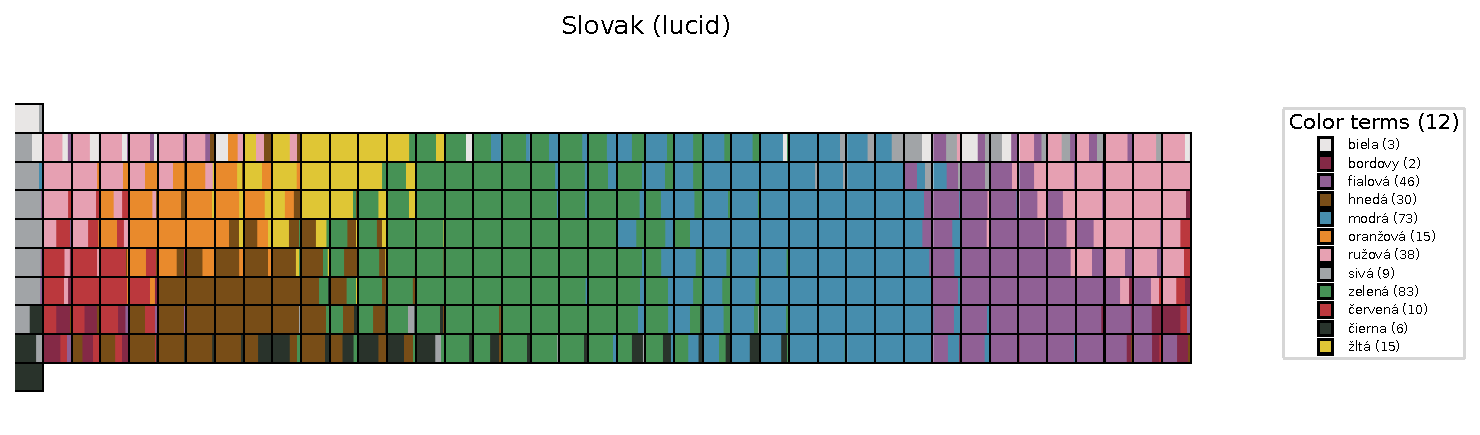
\includegraphics[page=1, width=\linewidth]{images/mode_maps/Slovak (lucid).pdf}
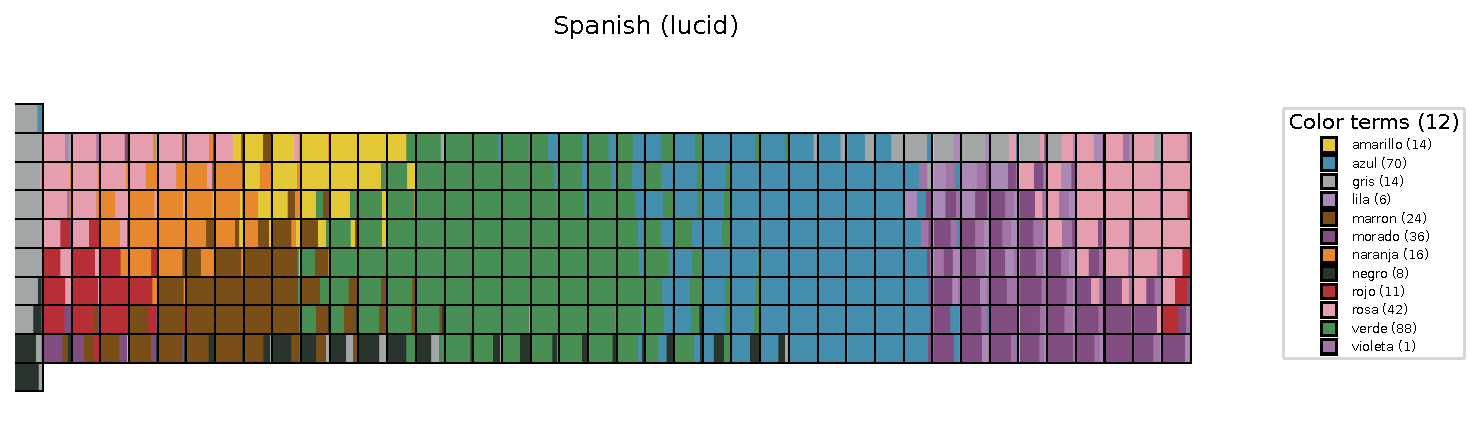
\includegraphics[page=1, width=\linewidth]{images/mode_maps/Spanish (lucid).pdf}
\caption[Proportion Maps (Russian, Serbian, Slovakian, Spanish)]{Proportional maps for Russian, Serbian, Slovakian, Spanish and respective color terms.}
\label{fig:color_maps_4}
\end{figure}

\begin{figure}[htbp]
\centering
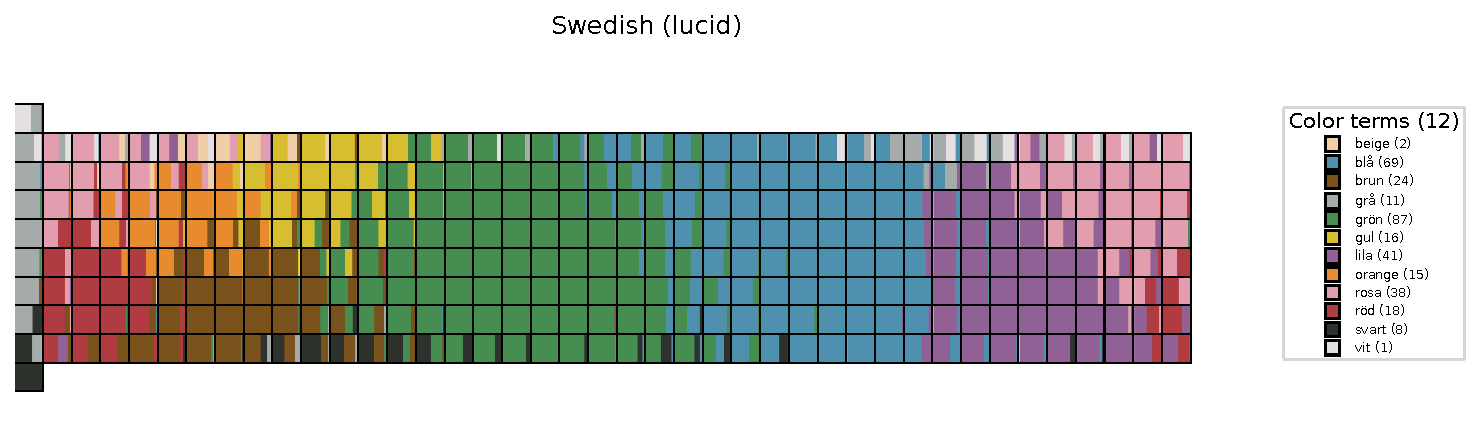
\includegraphics[page=1, width=\linewidth]{images/mode_maps/Swedish (lucid).pdf}
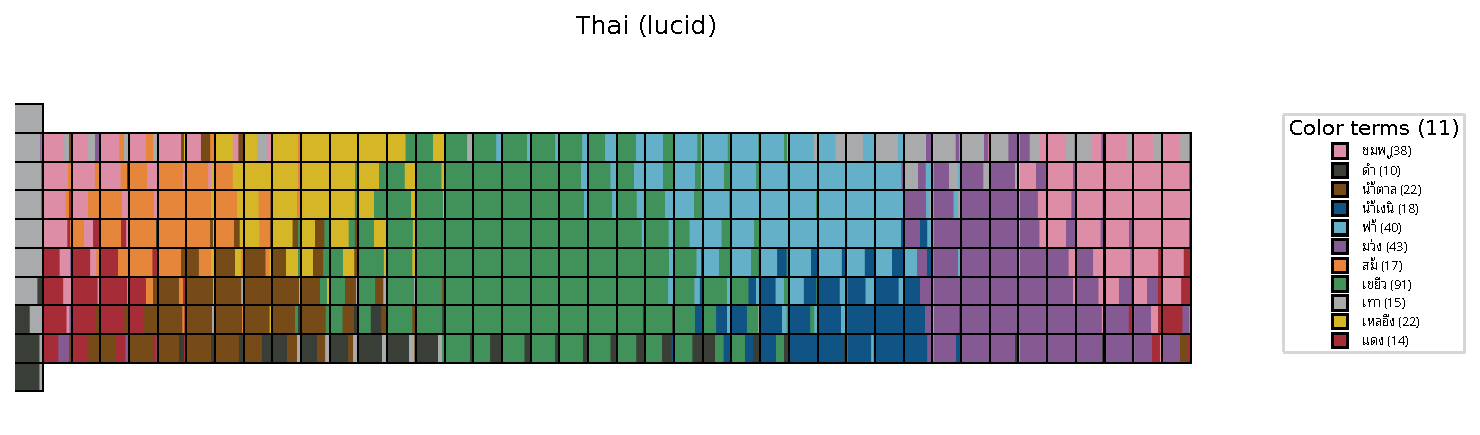
\includegraphics[page=1, width=\linewidth]{images/mode_maps/Thai (lucid).pdf}
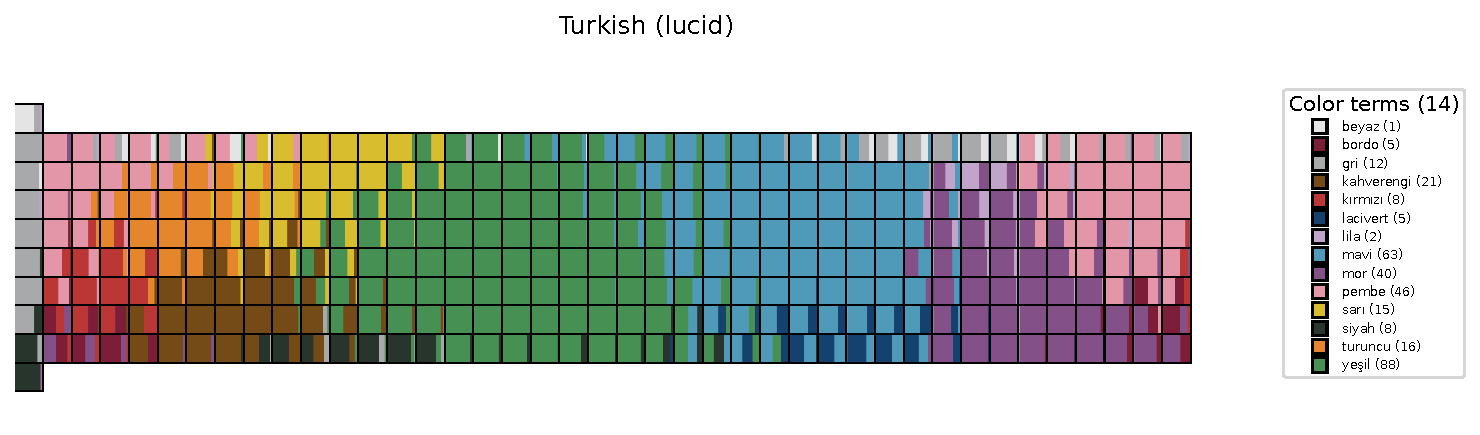
\includegraphics[page=1, width=\linewidth]{images/mode_maps/Turkish (lucid).pdf}
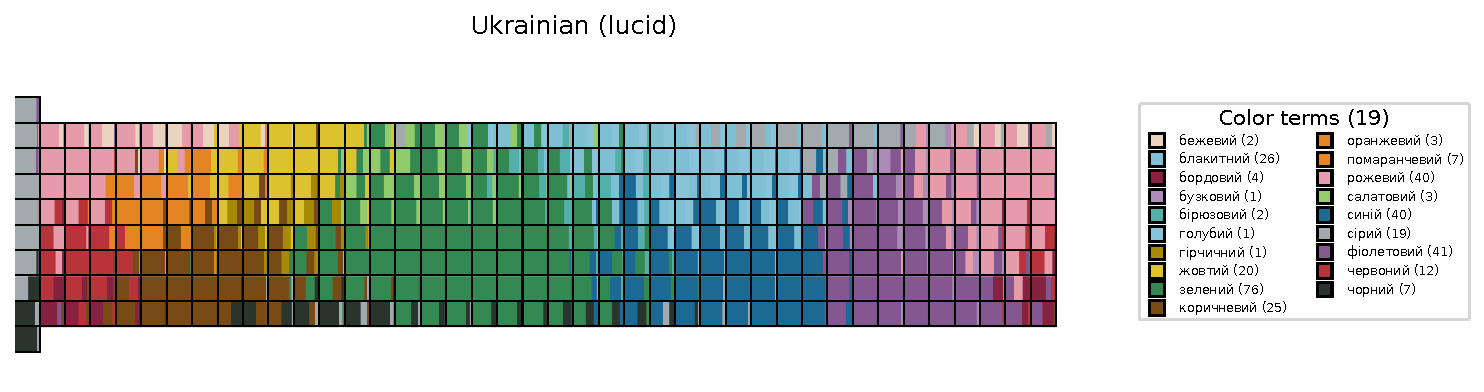
\includegraphics[page=1, width=\linewidth]{images/mode_maps/Ukrainian (lucid).pdf}
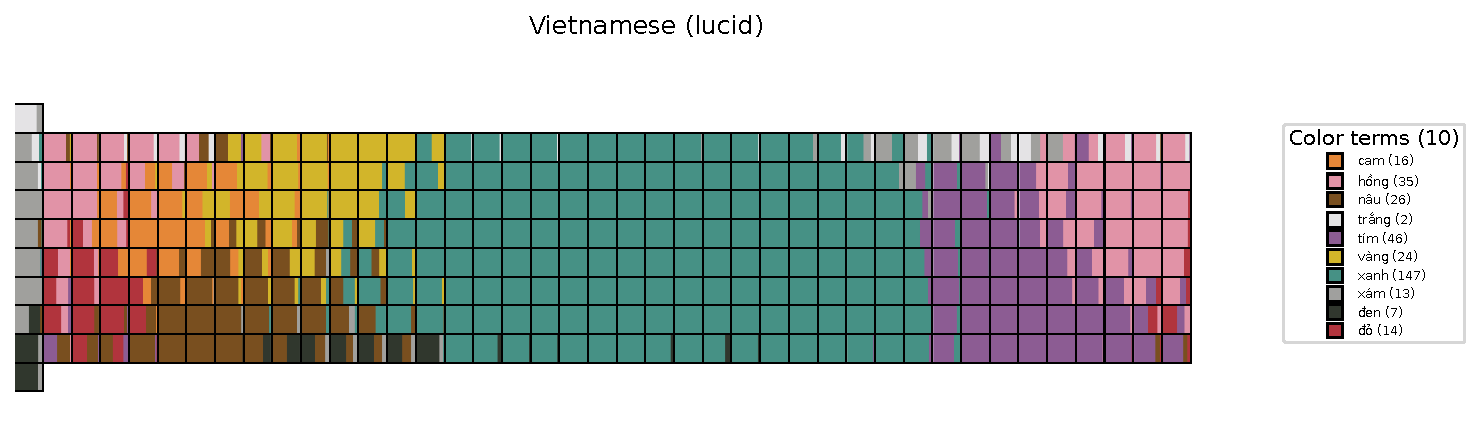
\includegraphics[page=1, width=\linewidth]{images/mode_maps/Vietnamese (lucid).pdf}
\caption[Proportion Maps (Swedish, Thai, Turkish, Ukrainian, Vietnamese)]{Proportional maps for Swedish, Thai, Turkish, Ukrainian, Vietnamese and respective color terms.}
\label{fig:color_maps_5}
\end{figure}


\subsection{Relations between languages}

\begin{figure}[h!t]
\centering
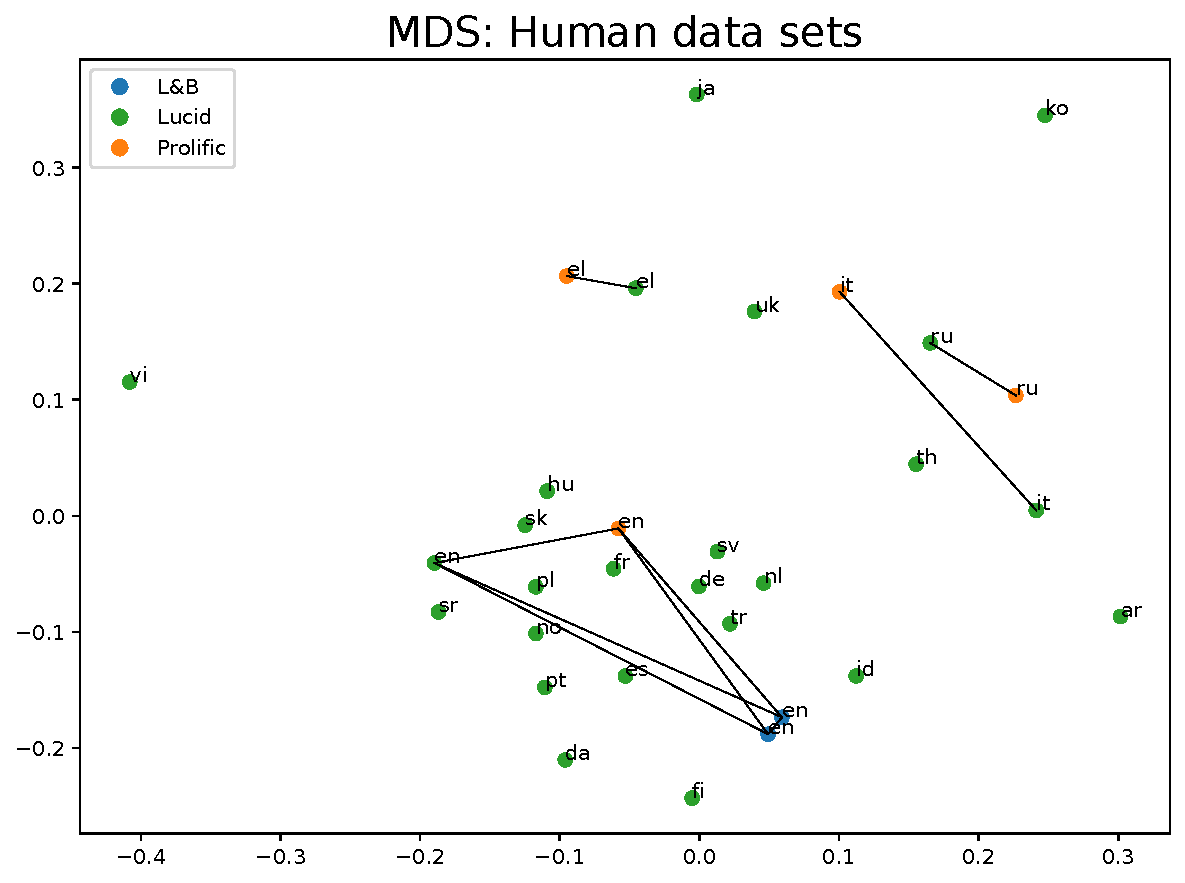
\includegraphics[page=1, width=0.49\linewidth]{images/MDS/mds_rand_index_human.pdf}
\hfill
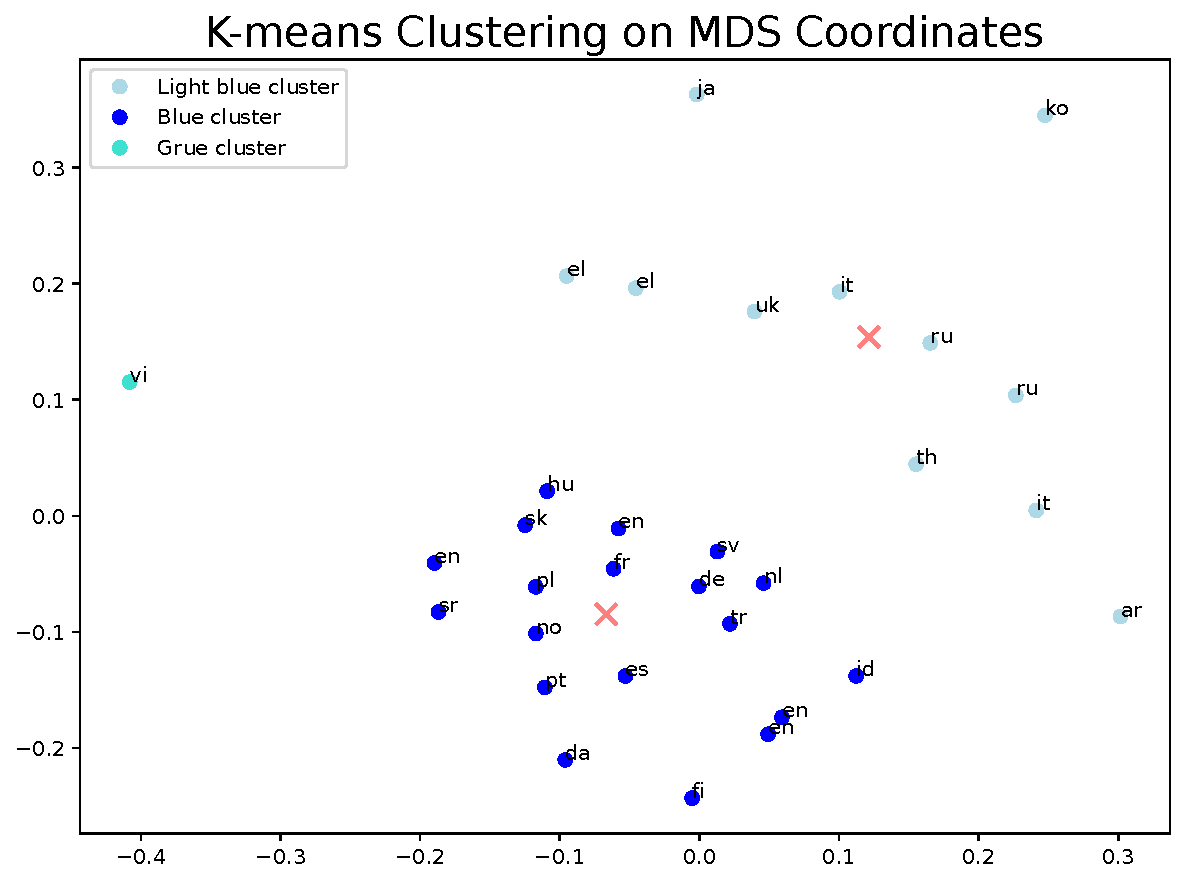
\includegraphics[page=1, width=0.49\linewidth]{images/MDS/kmeans_human.pdf}
\decoRule
\caption[MDS human data]{MDS human data. Left panel: MDS embedding based on the ARI matrix of human data (Lucid, Prolific, WCS) with lines connecting data points of the same language but different sources.
Right panel: K-means clustering (k=2) of MDS coordinates distinguishes two clusters: one representing languages with a distinct light blue category and another with a singular broad blue category.
The cluster centers are denoted by the red crosses.
Notably, Vietnamese, marked in a unique color, deviates due to its 'grue' category that merges green and blue hues.}
\label{fig:MDS_human}
\end{figure}



When observing the Rand Index Matrix directly, it is not possible to compare similarity and difference between color terms usage, as the Rand index simply provide overall distance score for each pair.
A multidimensional scaling (MDS) approach may be used to reveal the latent structure of the Rand matrix \parencite{shepard1980multidimensional}. Embedding the rand index values as a dissimilarity matrix into an MDS visually reveals the clustering of different languages and give more intuitive understanding about the similarities and dissimilarities across languages (Fig. \ref{fig:MDS_human}).
As expected, data of the same languages but different recruiters (el, ru, it, en) are mapped relatively close to each other. 
Furthermore, the constellation of languages in the MDS appears to be divided into three clusters.
First, Vietnamese is a special outlier placed in the periphery. This might be due to the large xanh category combining blue and green (grue) and a low overall number of 5.96 color terms in the lexicon (calculated as the exponent of the global entropy).
Second, a group of languages namely Hungarian, Slovakian, Serbian, Norwegian, Polish, French, Portuguese, Danish, Spanish, Swedish, Dutch, German, Turkish, Indonesian and Finish form a cluster which generally aligns strongly with the English lexicon. 
All these lexicon do distinguish between green and blue and have a mean of 8.06 [7.40, 8.73] color terms.
Additional categories to the eleven BCT are not major categories.
I will refer to this cluser as the blue cluster.
However, within the cluster different grouping tendencies can be described. 
Danish and Finish located at one extreme of the cluster both share a large red category (Finnish: punainen, Danish: rød) instead of differentiated between red and pink which is very small for Danish and Finnish. For both languages we detected a high usage of compound words (e.g. Finish: light red = vaaleanpunainen, Danish:light red = lys rød). The large red category result due to our heuristics to resolve compound words by replacing them with the base. 
Hungarian is located on the opposite side of the cluster. Reason for this might be an additional small category for dark red - bordó.


The third cluster consists of Greek, Ukraine, Japanese, Italian, Russian, Thai and Arabic.
A distinctive characteristic of these languages is the universal categorization of a 'light blue' hue, accompanied by an average lexicon comprising 10.70 [8.59, 12.81] color terms, indicative for a broadened chromatic vocabulary.
In the following I will refer to this groupe as the “light blue” cluster.
Languages of this cluster contain additional color categories in different parts of color space which makes it hard to categorize the relative position within the language.

K-means algorithm of the \textit{sklearn} library successfully distinguishes two clusters but fails to detect Vietnamese as a third cluster presumably because it is just one language (Fig. \ref{fig:MDS_human}).
The light blue cluster has a mean bootstrapped ARI to the English data of .59 (sd=.07) whereas the blue category has a higher ARI of .75 (sd=.06).




% % \section{Comparison Human and GPT4 and GPT4-V}

% \begin{figure}[h!t]
% \centering
% 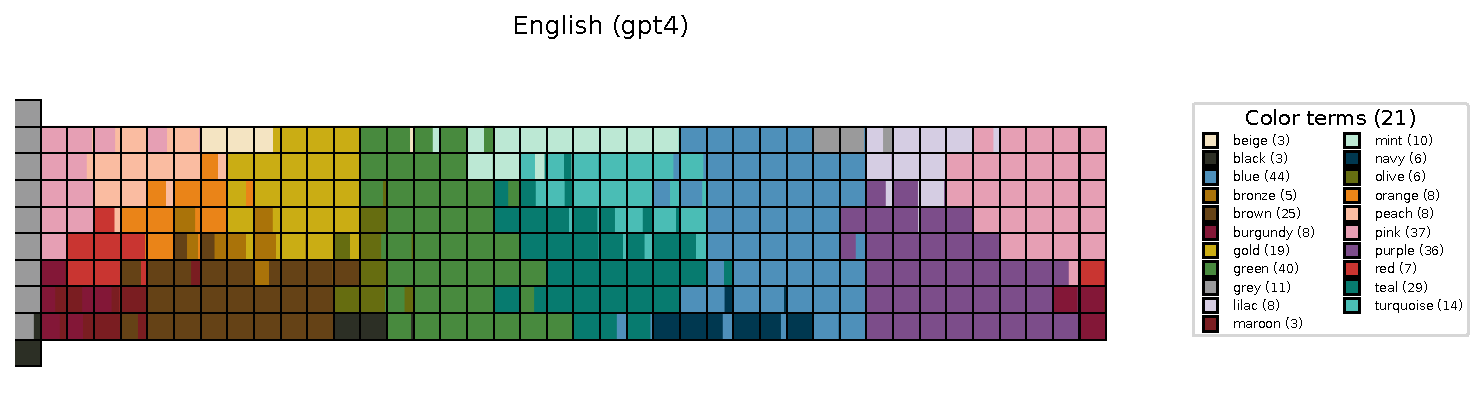
\includegraphics[width=\linewidth]{images/mode_maps_gpt4/English (gpt4).pdf}
% \hfill
% 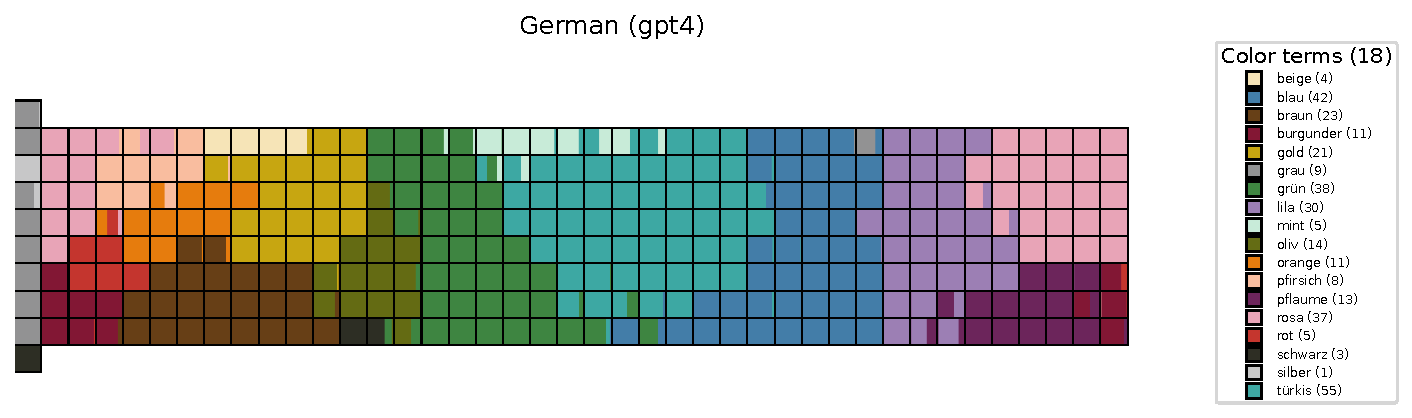
\includegraphics[width=\linewidth]{images/mode_maps_gpt4/German (gpt4).pdf}
% 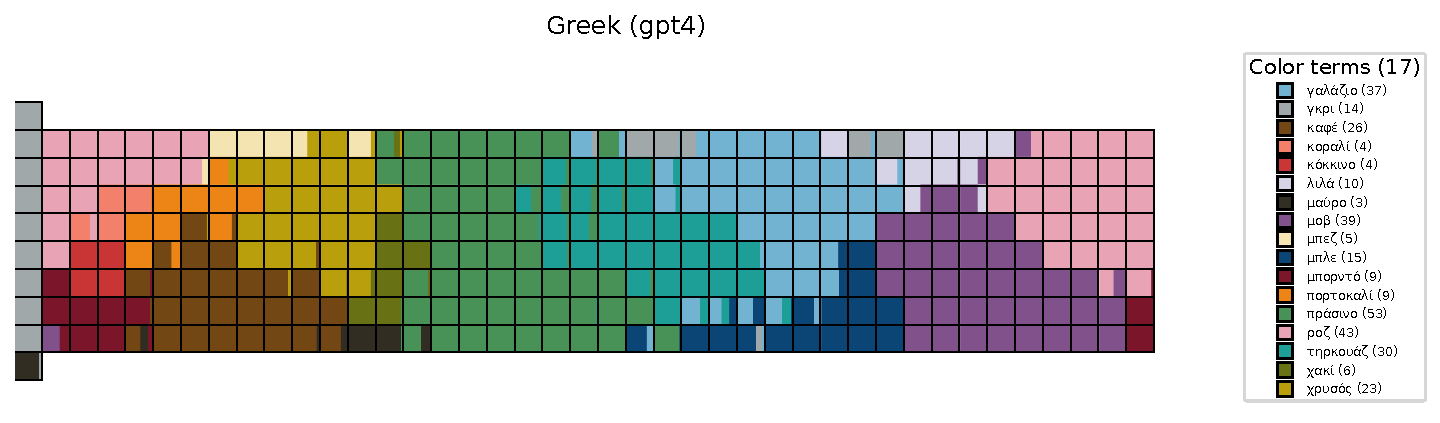
\includegraphics[width=\linewidth]{images/mode_maps_gpt4/Greek (gpt4).pdf}
% 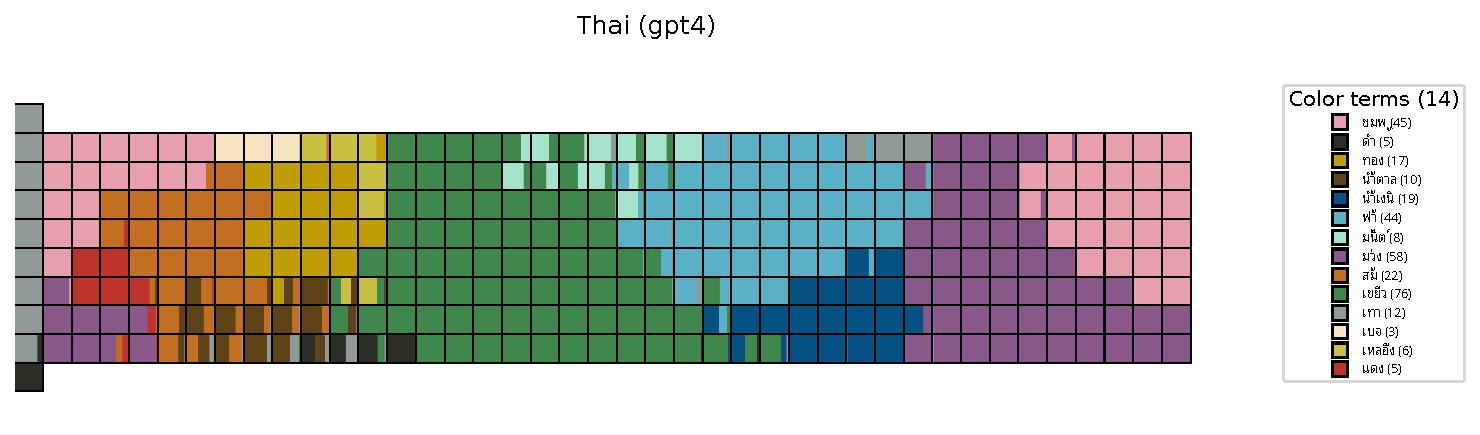
\includegraphics[width=\linewidth]{images/mode_maps_gpt4/Thai (gpt4).pdf}
% 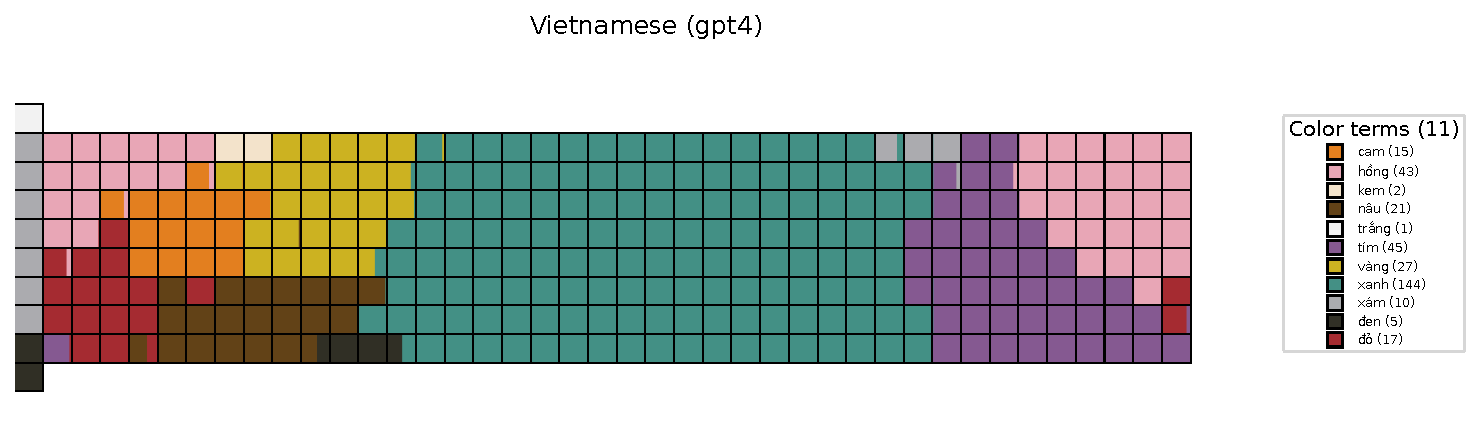
\includegraphics[width=\linewidth]{images/mode_maps_gpt4/Vietnamese (gpt4).pdf}
% \caption[GPT Proportion Plots]{Proportion plots for English, German, Greek, Thai, Vietnamese elicited from GPT4}
% \label{fig:mode-maps-gpt}
% \end{figure}

% \begin{figure}[h!t]
% \centering
% 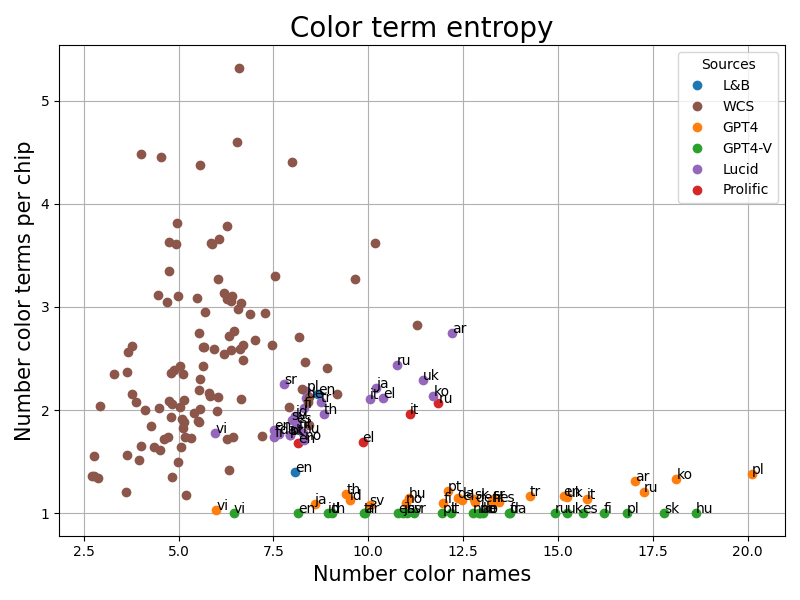
\includegraphics[page=1, width=\linewidth]{images/MDS/entropy-plot.png}
% \decoRule
% \caption[Entropy Plot]{}
% \label{fig:entropy_plot}
% \end{figure}

% \begin{figure}[h!t]
% \centering
% 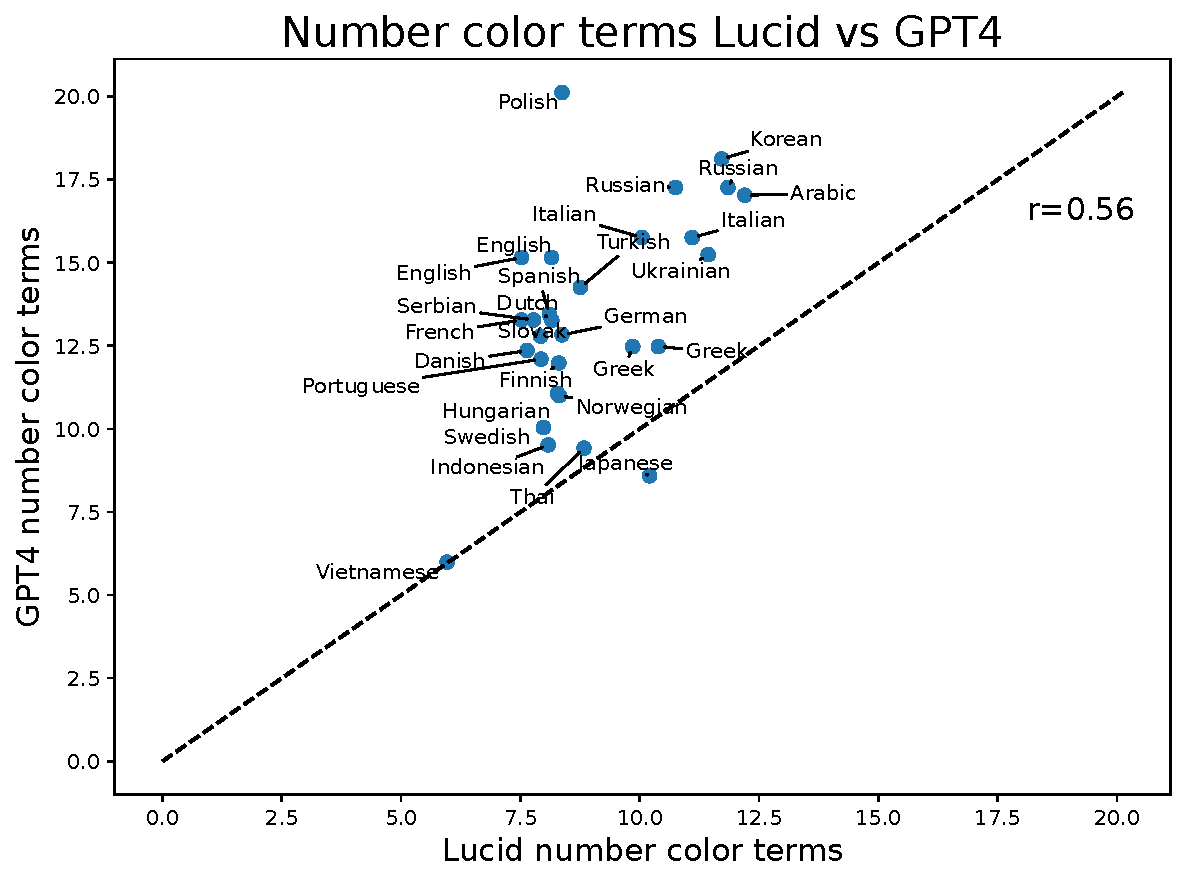
\includegraphics[page=1, width=\linewidth]{images/human_vs_gpt4.pdf}
% \decoRule
% \caption[Number Color Terms: GPT4 vs Human]{}
% \label{fig:human_vs_gpt4}
% \end{figure}

% \begin{figure}[h!t]
% \centering
% 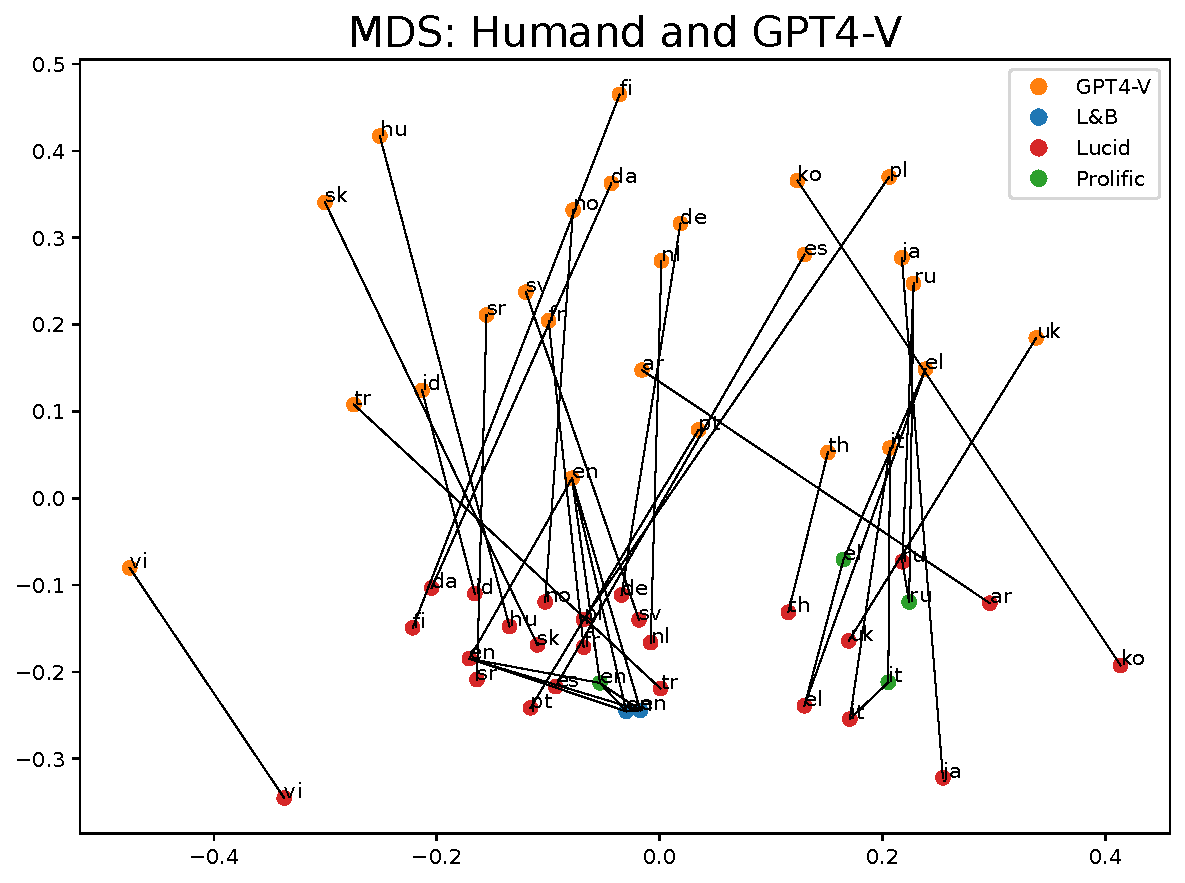
\includegraphics[page=1, width=0.49\linewidth]{images/MDS/mds_rand_index_human_gpt4-v.pdf}
% \hfill
% 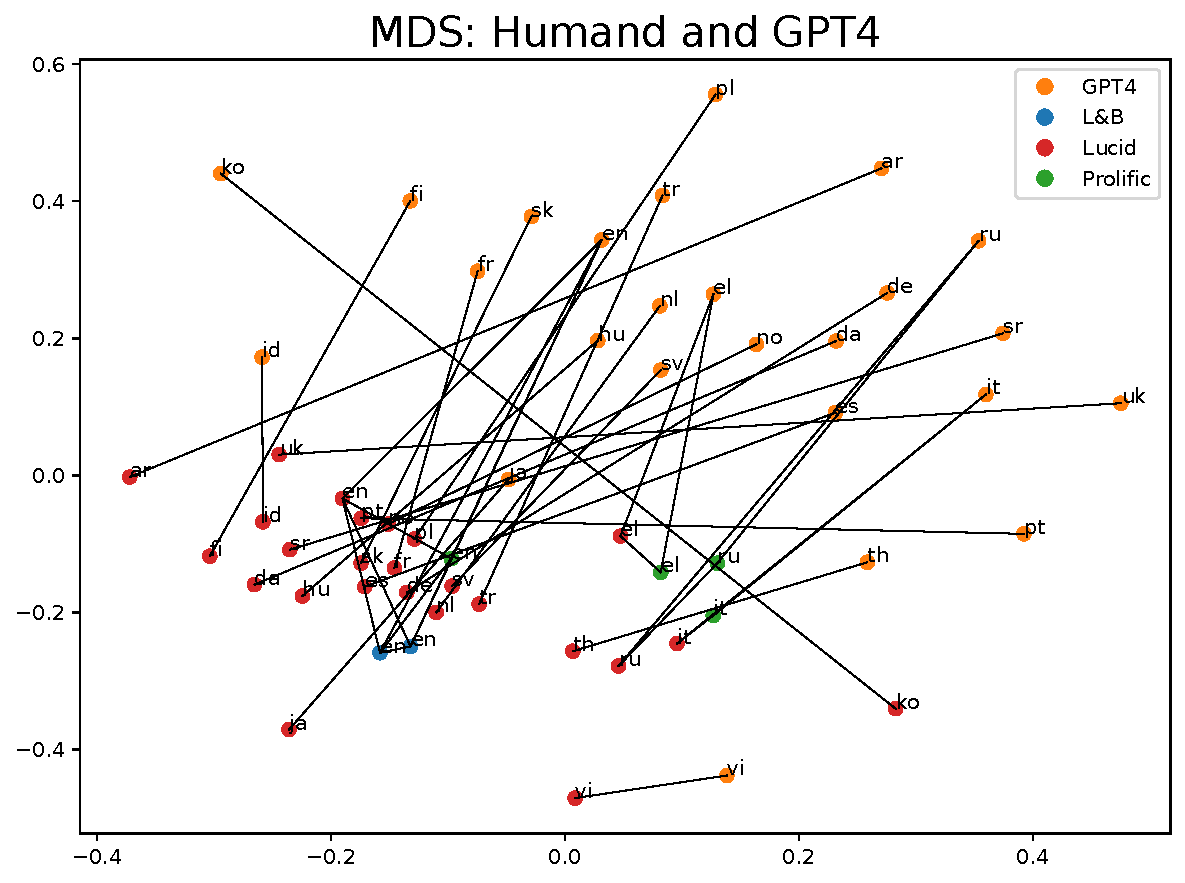
\includegraphics[page=1, width=0.49\linewidth]{images/MDS/mds_rand_index_human_gpt4.pdf}
% \decoRule
% \caption{}
% \label{fig:MDS_human-gpt}
% \end{figure}


% The proportional plots of the GPT4 data exhibit similar but more detailed naming pattern than the human data (Fig. \ref{mode-maps-gpt}.
% For English the BCT are present but subdivided by additional niche categories such as mint, navy, olive, teal and turquoise in the blue and green area. This results in a richer color lexicon of eleven additional terms compared to the human data (global entropy).
% The plots also illustrate low entropy in the responses for each chip (local entropy). Compared to human data, the individual chips show fewer different colors, reflecting a more uniform way of responding.

% Fig. \ref{fig:entropy_plot} illustrates the relationship between the local entropy on the y-axis representing consensus across answers for the single chips and the global entropy on the x-axis defined as the number of color terms in the overall dataset (exponent of the entropy on all chips).
% The different datasets cluster in different areas of the plot highlighting different naming behaviour for GPT4, GPT4-V, WCS and the collected dataset.

% The observations from above get reflected in this plot. GPT4 (orange) data cluster around regions of low local entropy reflecting the highly deterministic naming manner.
% For GPT4-V (green) we only have one answer per color which is why the local entropy equals one for all languages.
% Both human datasets cluster around higher values of local entropy. 
% The languages of the collected data (purple) use significantly more diverse color names per chip compared to GPT4 and GPT4-V (W = .0, p < 0.001 and W = .0, p < 0.001 using Wilcoxon-Rank test).
% In contrast examination of the number of color terms (global entropy, Fig. \ref{human_vs_gpt4}) used by GPT4 and GPT4-V is significantly higher than in the collected human data (W = .0, p < 0.001 and W = .0, p < 0.001 using Wilcoxon-Rank test).
% % Or: (Wilcoxon signed rank test: t(24) = 5.0, p < 0.001, and t(24) = 3.0, p < 0.001)
% However, we see that the number of color categories tend to be correlated across GPT-4-V and humans (r =.09) but not across GPT-4 and humans (r=.55), indicating that languages with a small number of categories in humans (such as Vietnamese) also tend to have fewer categories in GPT-4-V and vice versa.

% When comparing the human data we see a significant higher number of color terms in the newly collected data (9.02 [5.92, 12.12]) than in the WCS data (5.71 [2.57, 8.85]; p < 0.001)







% Also, on a single language level, humans fairly overlap with the labels proposed by GPT-4 (mean: 59\%, SD: 16\%), and the overlapping
% colors occur at a similar frequency except for Arabic (r = .06)
% and Dutch (r = .32) (.44-.90, mean: .65, SD: .13).



\section{Comparison Human and GPT4 and GPT4-V}

\begin{figure}[h!t]
\centering
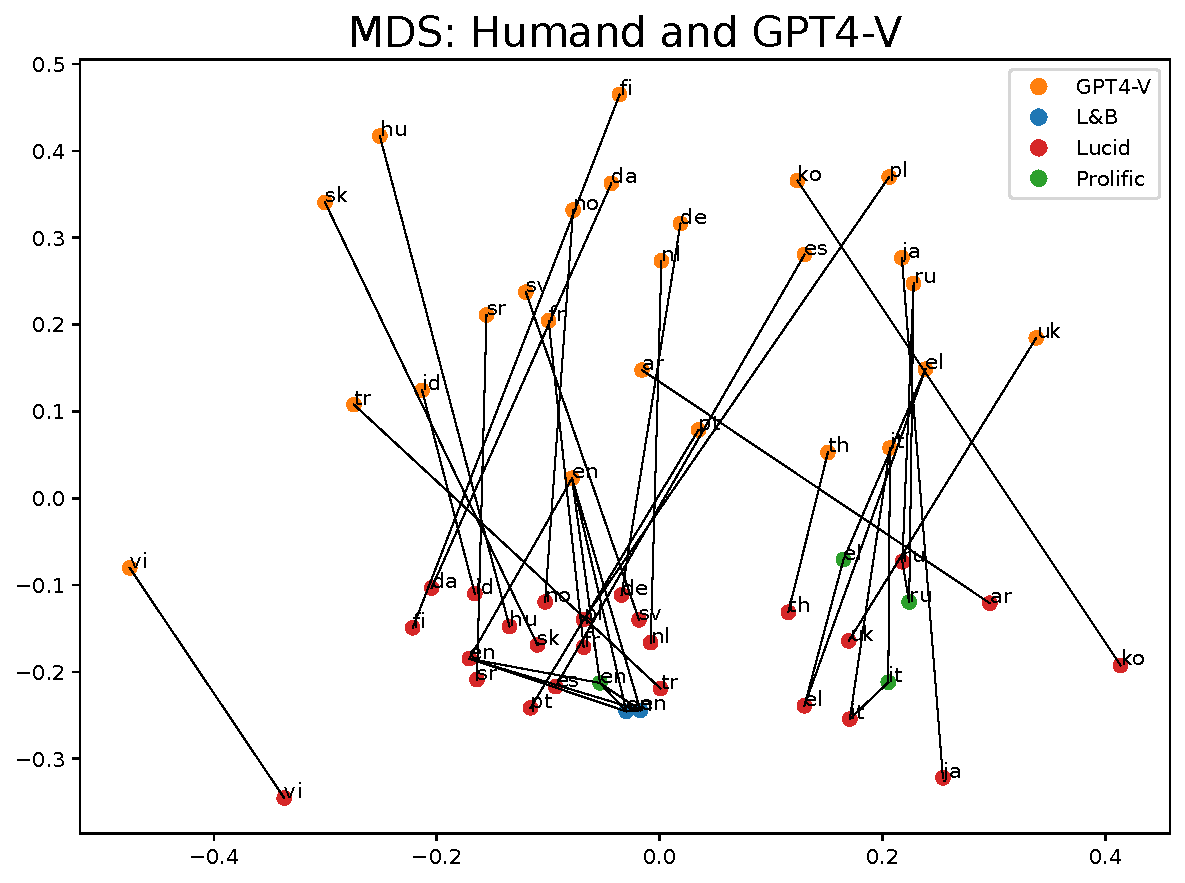
\includegraphics[page=1, width=0.49\linewidth]{images/MDS/mds_rand_index_human_gpt4-v.pdf}
\hfill
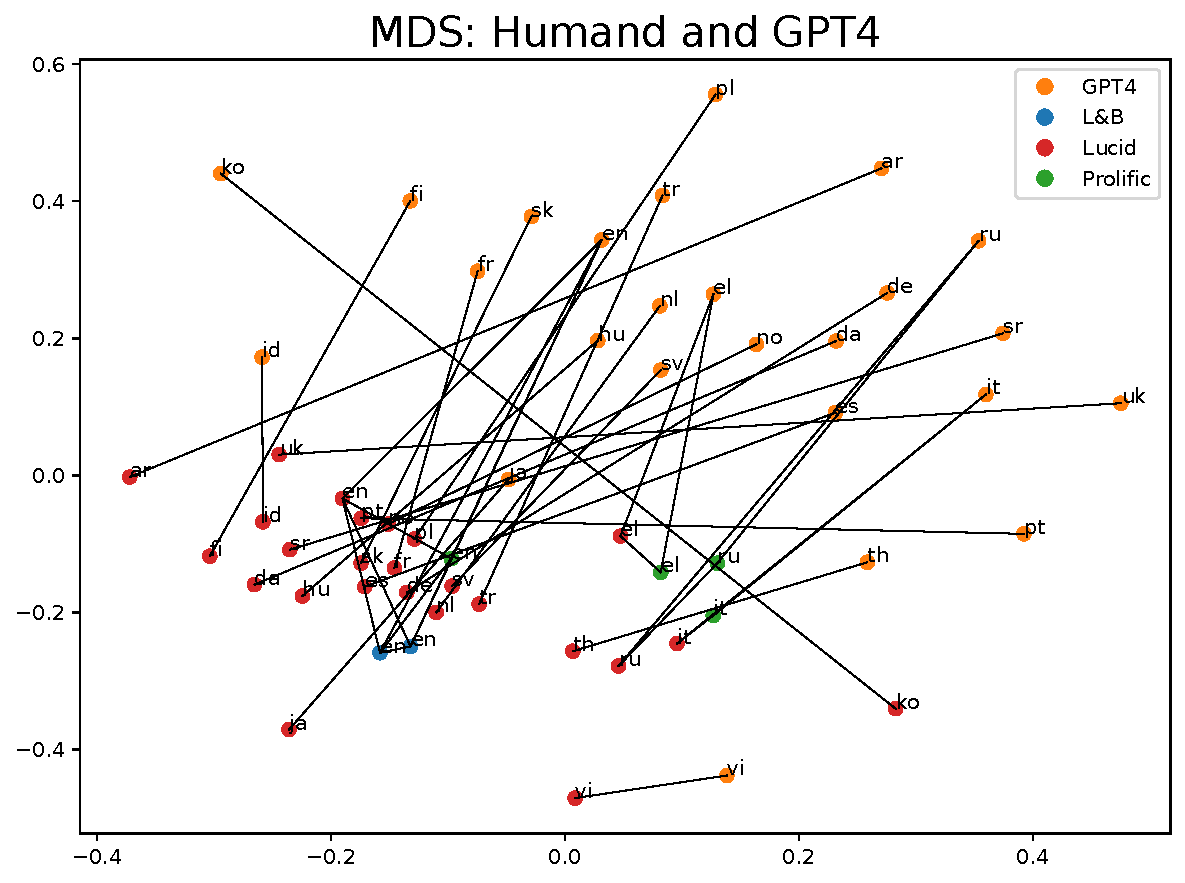
\includegraphics[page=1, width=0.49\linewidth]{images/MDS/mds_rand_index_human_gpt4.pdf}
\decoRule
\caption[MDS ARI Lucid \& GPT4/GPT4-V]{MDS human and GPT4/GPT4-V.
MDS embedding visualizes ARI matrix of human data sets and GPT4-V (left panel) and GPT4 (right panel). To highlight the comparison between different sources identical languages are connected by lines.
The clear division along the y-axis in both panels suggests it acts as a discriminator between human and GPT4 datasets.
The language pairs tend to be aligned along the dividing line which becomes visually apparent with the tendency of the lines to cross the border in a orthogonal way.
Notably, for GPT4-V, language pair positions exhibit a significant correlation which was not reproduced in the human - GPT4 plot(mainly due to outliers like Korean and Arabic.}
\label{fig:MDS_human_gpt}
\end{figure}

To investigate similarities and differences across the human and GPT4 data Fig \ref{fig:MDS_human_gpt} shows an MDS taking a distance matrix calculated from the ARI matrix as input. This MDS differs from the one shown above since we now use both human and GPT4 data. 
The plots make it visually apparent that human and GPT4 or GPT4-V data cover different parts of the MDS space.
However, the corresponding languages seem to be similarly aligned along the dividing border. This gets qualitatively apparent as the connecting lines between the same languages in the two data sets cross the dividing border in a predominantly orthogonal manner. In the GPT4 plot the y-axis is correlated with the position of the languages pairs (r=.45, p=.025; if we exclude the outlier Korean, correlation is even higher: r=.56, p=.004). Visually apparent correlation on the x-axis does not reach significance due to strong outliers like Korean, Arabic and Ukrainian.
For GPT4-V the position of the languages is correlated along the x-axis (r=.67, p < .000). The following can be derived from this: First, the two data sets obtained from humans and GPT4 or GPT4-V are fundamentally different from each other as they group into separate clusters. Second, the correlation of the relative positions of the single languages in the subgroups highlights the preserved similarity across the data sets for single languages.

\begin{figure}[h!t]
\centering
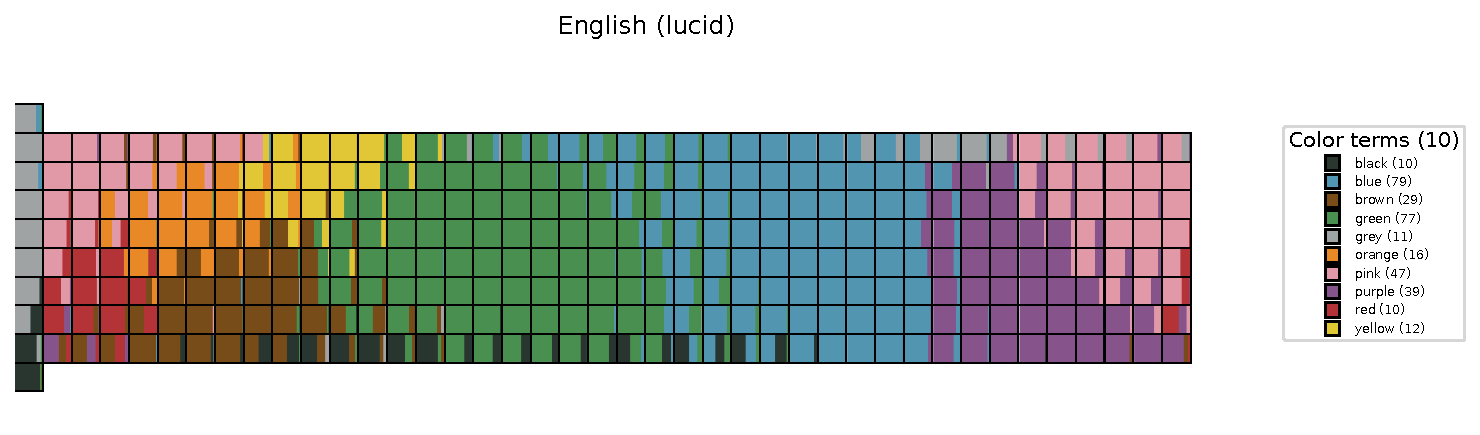
\includegraphics[width=0.49\linewidth]{images/mode_maps/English (lucid).pdf}
\hfill
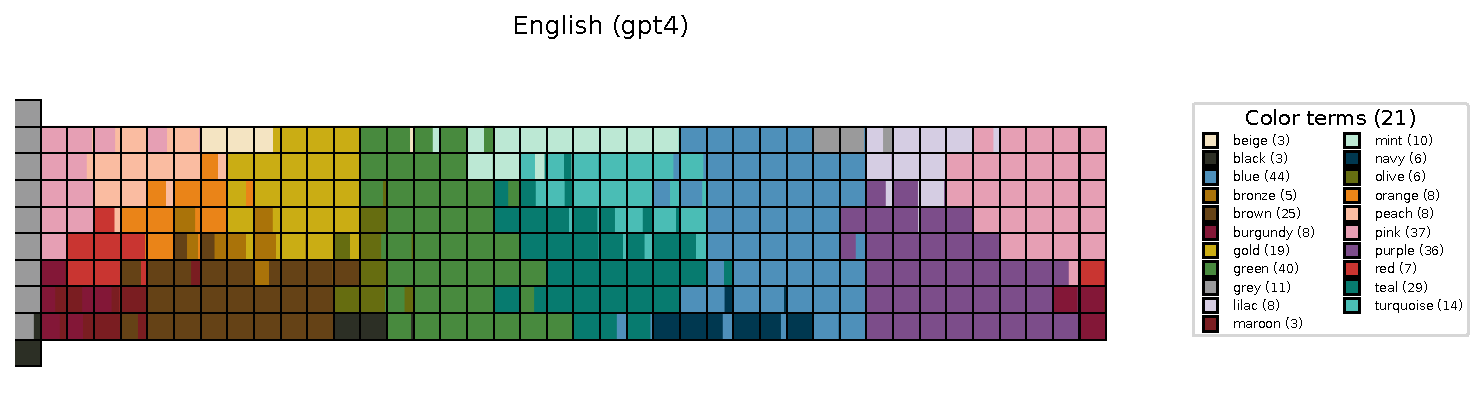
\includegraphics[width=0.49\linewidth]{images/mode_maps_gpt4/English (gpt4).pdf}
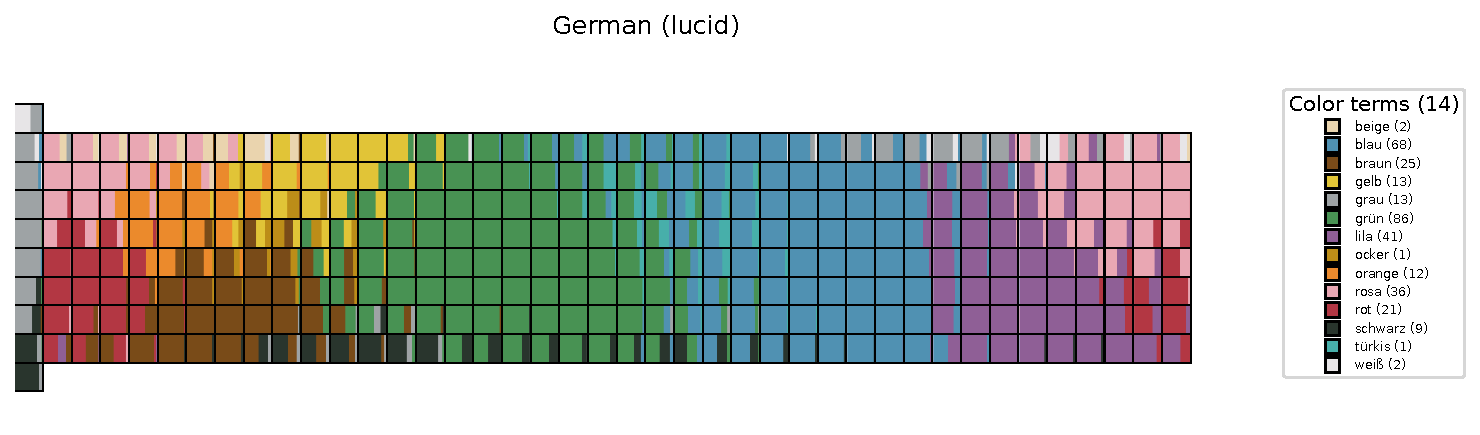
\includegraphics[width=0.49\linewidth]{images/mode_maps/German (lucid).pdf}
\hfill
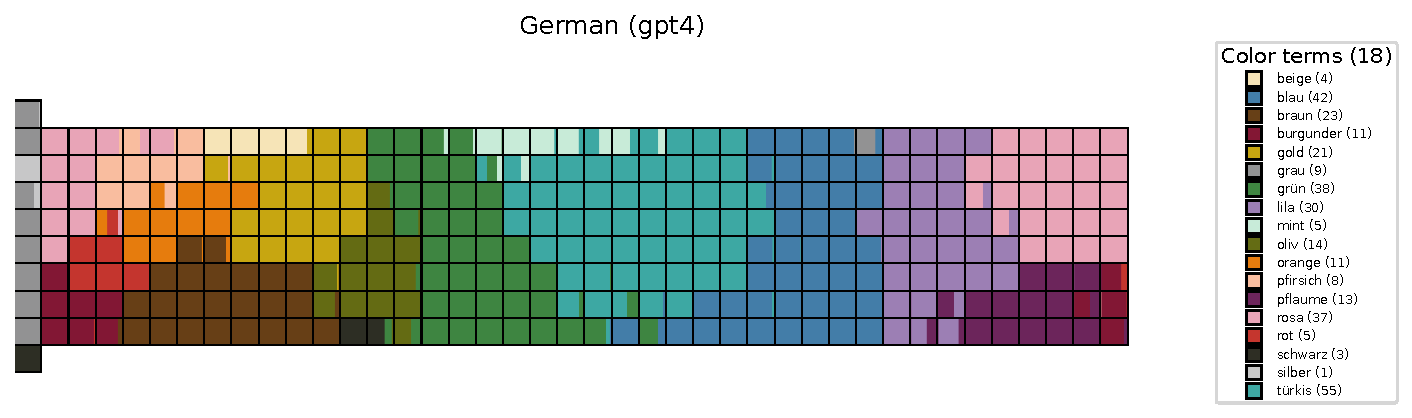
\includegraphics[width=0.49\linewidth]{images/mode_maps_gpt4/German (gpt4).pdf}
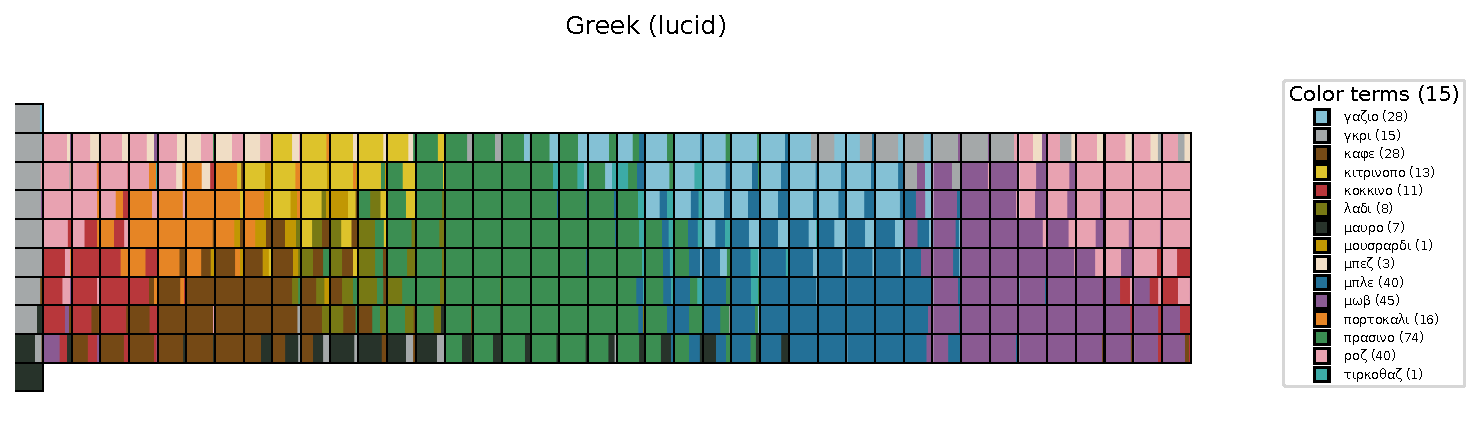
\includegraphics[width=0.49\linewidth]{images/mode_maps/Greek (lucid).pdf}
\hfill
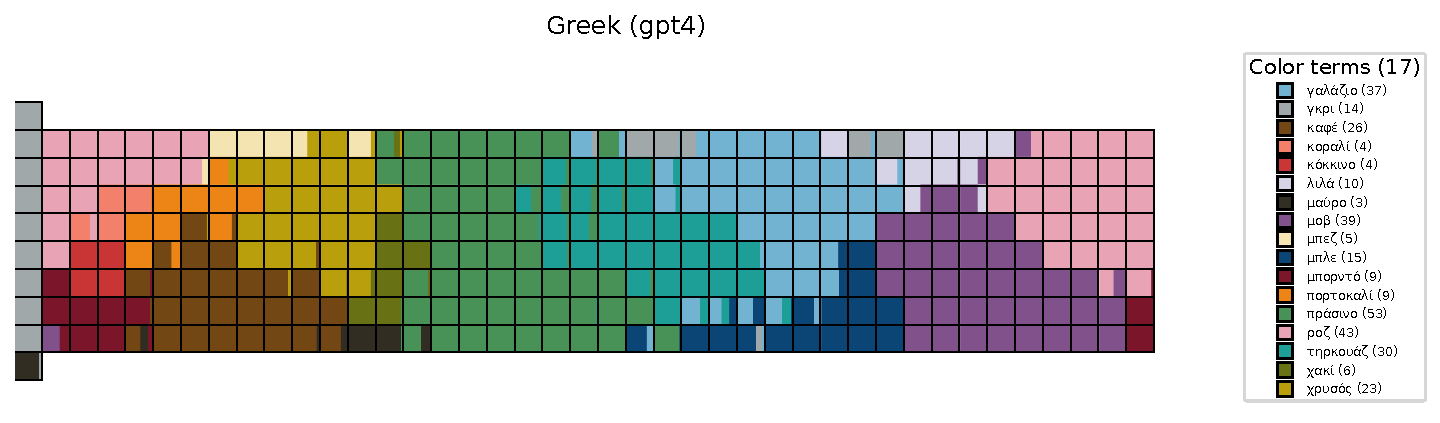
\includegraphics[width=0.49\linewidth]{images/mode_maps_gpt4/Greek (gpt4).pdf}
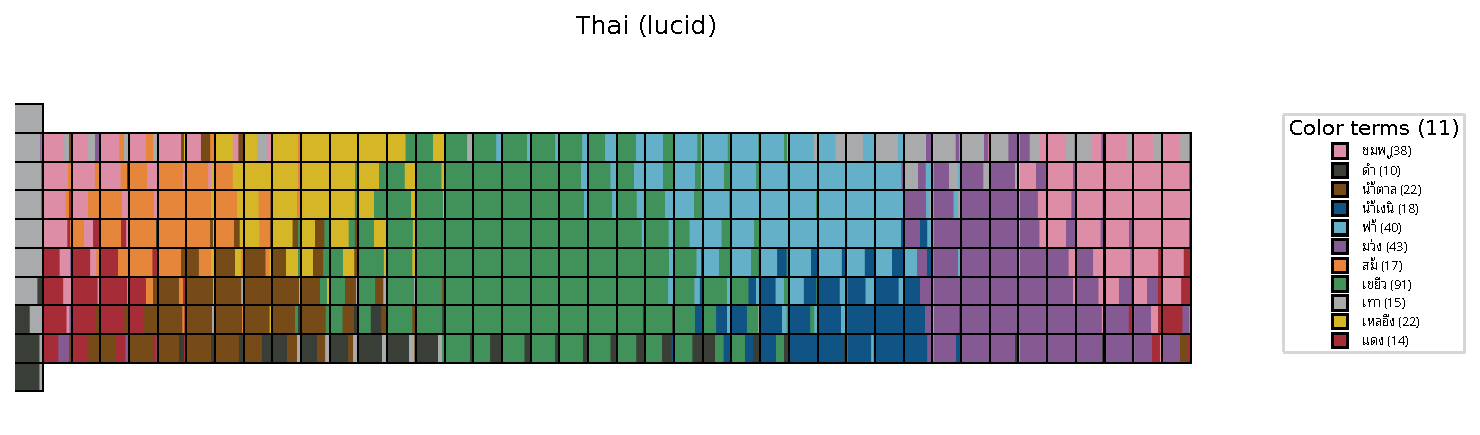
\includegraphics[width=0.49\linewidth]{images/mode_maps/Thai (lucid).pdf}
\hfill
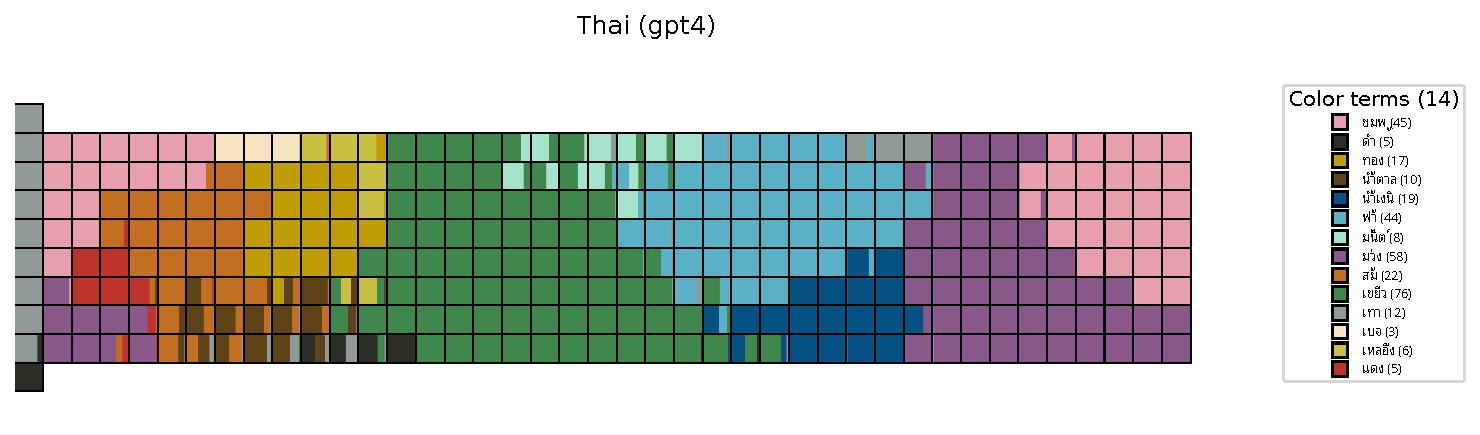
\includegraphics[width=0.49\linewidth]{images/mode_maps_gpt4/Thai (gpt4).pdf}
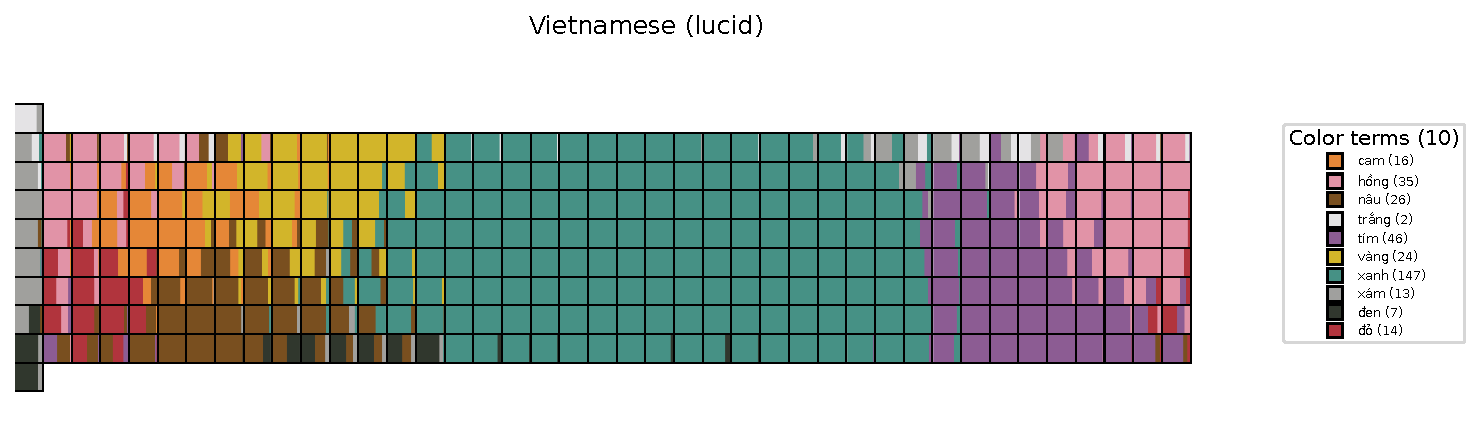
\includegraphics[width=0.49\linewidth]{images/mode_maps/Vietnamese (lucid).pdf}
\hfill
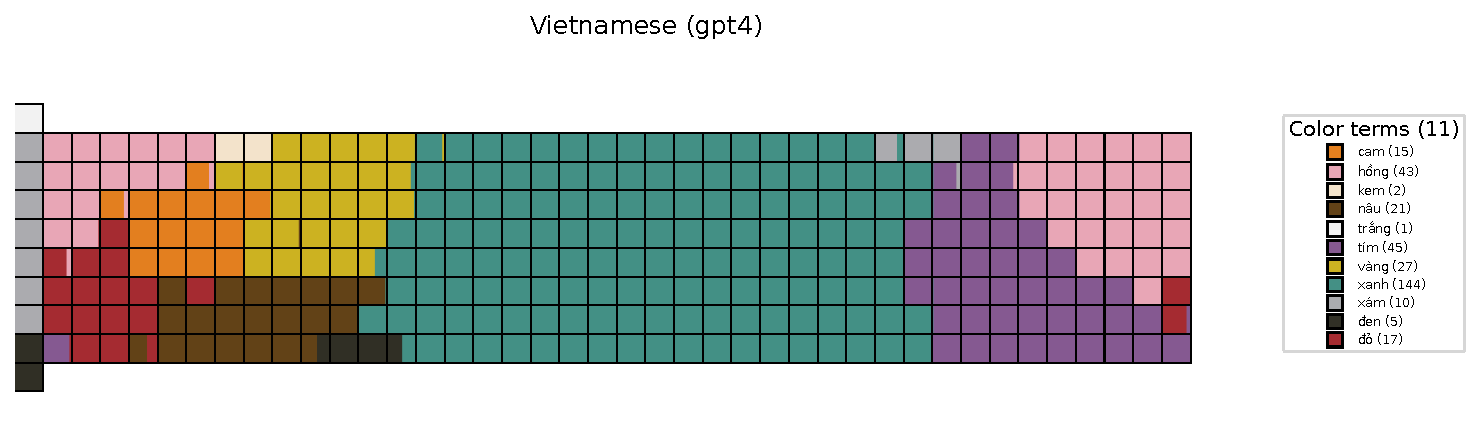
\includegraphics[width=0.49\linewidth]{images/mode_maps_gpt4/Vietnamese (gpt4).pdf}
\caption[Proportion Plots: GPT4 vs Human]{Proportion plots comparing color vocabularies for English, German, Greek, Thai, Vietnamese across human and GPT4 agents.}
\label{fig:mode-maps-human_vs_gpt}
\end{figure}


When qualitatively comparing GPT4 with human proportional plots the GPT4 data exhibit a similar but more detailed naming pattern. 
To compare data of GPT4 and Lucid, Fig. \ref{fig:mode-maps-human_vs_gpt} shows the proportional plots for English, German, Greek, Thai and Vietnamese side by side for both data sets.
Fig \ref{fig:mode-maps-gpt1} and \ref{fig:mode-maps-gpt2} show the full set of proportional plots for all languages elicited from GPT4.
For English the eleven BCT are present in the GPT4 data but subdivided by additional niche categories such as mint, navy, olive, teal and turquoise in the blue and green area. 
Turquoise is a very prominent category throughout most of the GPT4 data, even if the category is small or absent in the Lucid data (English, German, Greek).
Mint is also present in many languages of GPT4 data even if the word is not native to the languages (German, Thai, Danish, Dutch, Polish... E.g. \textthai{มิ้นต์} is the Thai writing for the English word mint and not a native Thai word).
In the case of English this results in a richer color lexicon of eleven additional terms compared to human data (global entropy). 
In Japanese however, GPT4 responds with a lower number of color terms. Especially, \japaneseText{ミズ色} the light blue category is absent.
The plots also illustrate low entropy in the responses for each chip (local entropy). Compared to human data, the individual chips show fewer different colors, reflecting a more uniform way of responding.
However, the comparison also reveals a tendency that languages such as Vietnamese which have a small color vocabulary in the human data also have fewer color terms listed for the GPT4 data. In contrast languages like German and Greek with larger color vocabularies also have higher numbers of color terms in the respective GPT4 Data.


\begin{figure}[h!t]
\centering
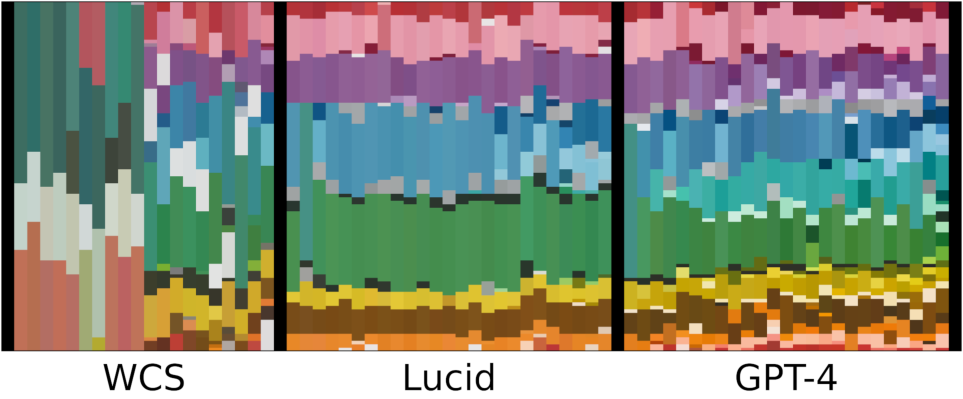
\includegraphics[page=1, width=\linewidth]{images/stream_plot.pdf}
\decoRule
\caption[Stream Plot]{Color Category Differentiation Across WCS, Lucid, and GPT4 Data Sets. This stream plot visualizes the evolution of color category vocabularies across WCS, Lucid, and GPT4 data sets, aligning languages by the number of color categories used, from those with fewer categories (left) to those with many (right). Specifically, for the WCS data set, only the 10 languages with the lowest and highest numbers of color terms are illustrated. This showcases a progression from languages utilizing as few as three color terms, similar to those observed in the WCS data set, to the more complex lexicons found in Lucid data. Remarkably, GPT4 data display a pronounced trend towards the segmentation of color space into very fine categories, exemplified by the emergence of turquoise as a distinct major color category.}
\label{fig:stream_plot}
\end{figure}

Fig \ref{fig:stream_plot} illustrates the number of color terms per collected language divided into the three examined data sets (For simplicity the GPT4-V data are not presented).
For the 110 languages in the WCS dataset the 20 languages with the lowest and highest number of color terms are depicted.
This visualization gives an intuitive understanding in how the three data sets differ. The WCS includes languages of very few color terms, essentially differentiating between warm, cold and light. It also contains languages with higher numbers of color terms overlapping in the number and size of the color categories in the collected data on Lucid. 
The GPT4 Data however show a growing differentiation far beyond the Lucid data.



\begin{figure}[h!t]
\centering
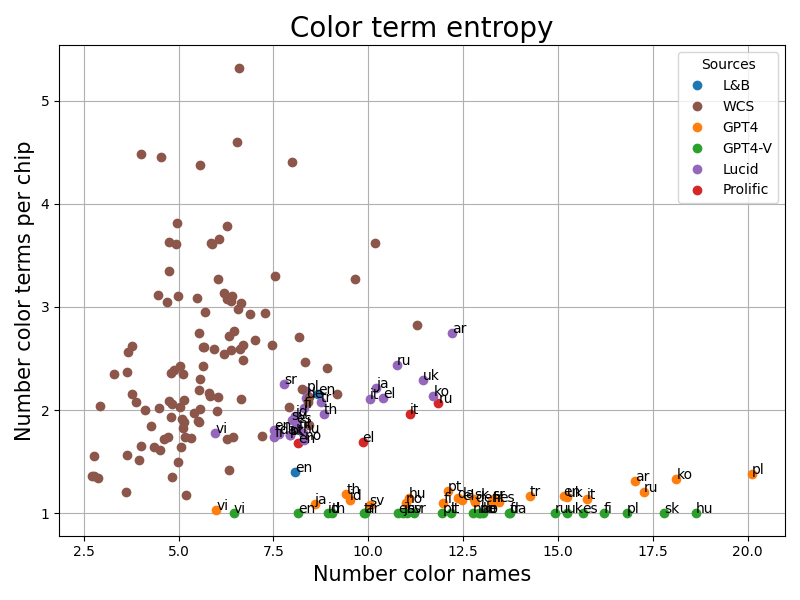
\includegraphics[page=1, width=\linewidth]{images/MDS/entropy-plot.png}
\decoRule
\caption[Entropy Plot]{Entropy Plot: Number of color terms for single chips (exp of local entropy) compared to number of color terms overall (exp. of global entropy) for WCS, Lucid, Prolific, GPT4, and GPT4-V.
GPT4 and GPT4-V exhibit relatively large color lexica and deterministic response behavior (Low local entropy in GPT4-V because of procedure).
Local entropy of human data (Lucid, Prolific, WCS, L\%B) is consistently higher and overlaps across data sets. 
Compared to the WCS, the other human datasets containing data from industrialized languages have larger color vocabularies. This supports \textcite{gibsonColor2017}'s hypothesis that industrialization may drive the development of new color terms.}
\label{fig:entropy_plot}
\end{figure}

Thus global vs. local entropy might drive the differences we see in the mixed MDS plots from above. This relationship is investigated on Fig \ref{fig:entropy_plot} which plots local entropy on the y-axis vs. global entropy on the x-axis. Global entropy here means the number of color terms computed as the exponent of the entropy on all chips.
Again we see distinct clusters for the data of the WCS, the newly collected data, GPT4 and GPT4-V.
The human data sets are adjacent but differ in the number of mean color terms significantly. As reported earlier the WCS languages cover a significant small number of color terms on average. The variance in both data sets are equally high (WCS=1.60, Lucid=1.58).
However, across all data sets the WCS data show the highest local entropy and therefore lowest consensus.

In contrast, the GPT4 data shows a more deterministic character. GPT4 and GPT4-V use significantly less diverse color names per chip compared to the collected human data ( p<.001 for both cases via Wilcoxon-Rank test).
The opposite effect can be observed for the total number of color term. The color lexicon of the GPT4 and GPT4-V data are significantly larger than for the human data ( p<.001 for both cases via Wilcoxon-Rank test).

\begin{figure}[h!t]
\centering
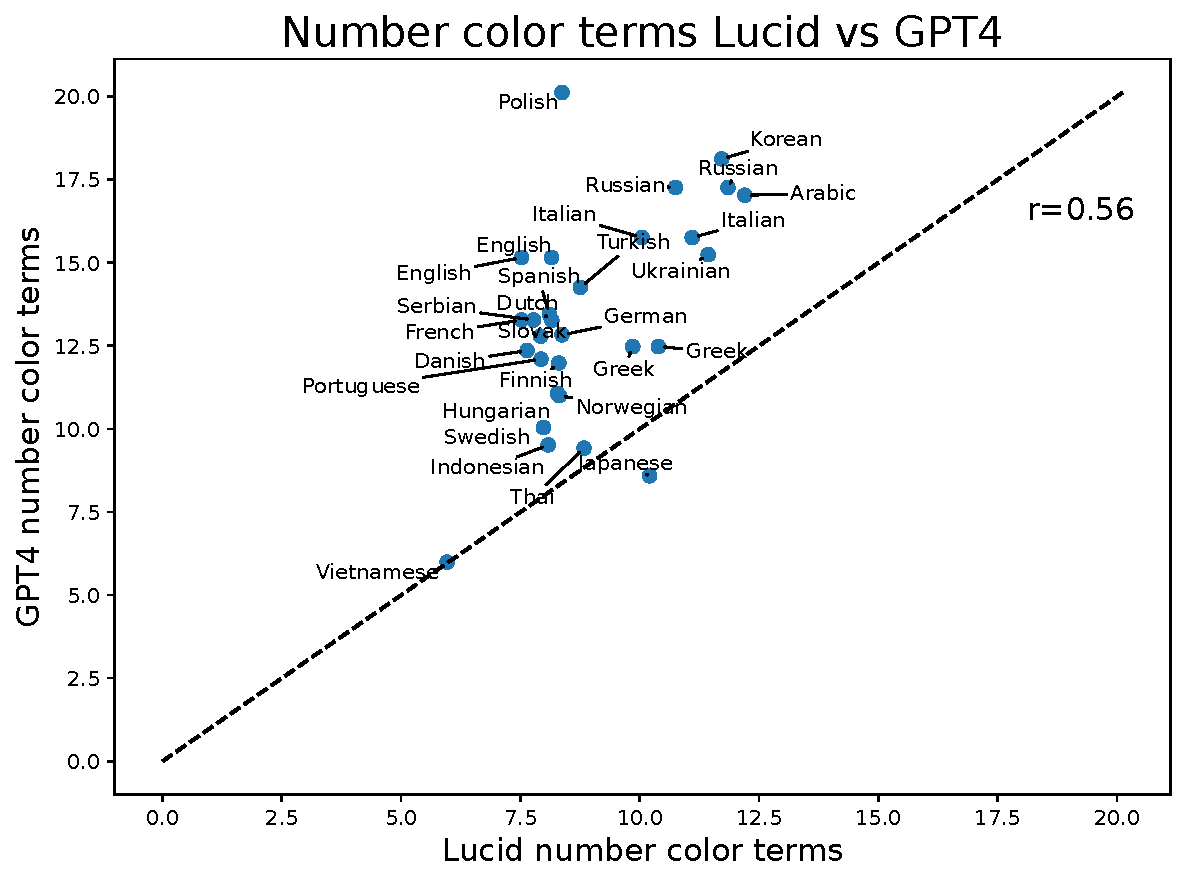
\includegraphics[page=1, width=\linewidth]{images/human_vs_gpt4.pdf}
\decoRule
\caption[Number of color terms]{Number of color terms across languages for Lucid and GPT4. Data indicate larger color vocabularies for GPT4 compared to Lucid data (except Japanese). However, the number of color terms is correlated across languages, proposing that languages with few color terms in Lucid data tend to have a smaller number of color terms in GPT as well.}
\label{fig:human_vs_gpt4}
\end{figure}

However, we see that the number of color categories tend to be strongly correlated across languages for GPT4 and humans (r=.56, p=.002, Fig. \ref{fig:human_vs_gpt4}) but rather weak across GPT4-V and humans (r=.14, p=.479). This indicates that languages with a small number of categories in humans (such as Vietnamese) also tend to have fewer categories in GPT4 and vice versa.
Japanese is one exception here. As mentioned earlier the GPT4 data do not even include the major light blue category. 

Moreover, high correlation of the global entropy with the y-axis in Fig. \ref{fig:MDS_human_gpt} was found for Lucid - GPT4 and Lucid - GPT4-V (r=.79, p<.000, r=.78, p<.000) highlighting that the difference between the two respective data sets are mainly based on the global entropy. 
For the x-axis correlation was lower but still significant (r=.51, p<.000, r=.32, p<.015).

\begin{figure}[h!t]
\centering
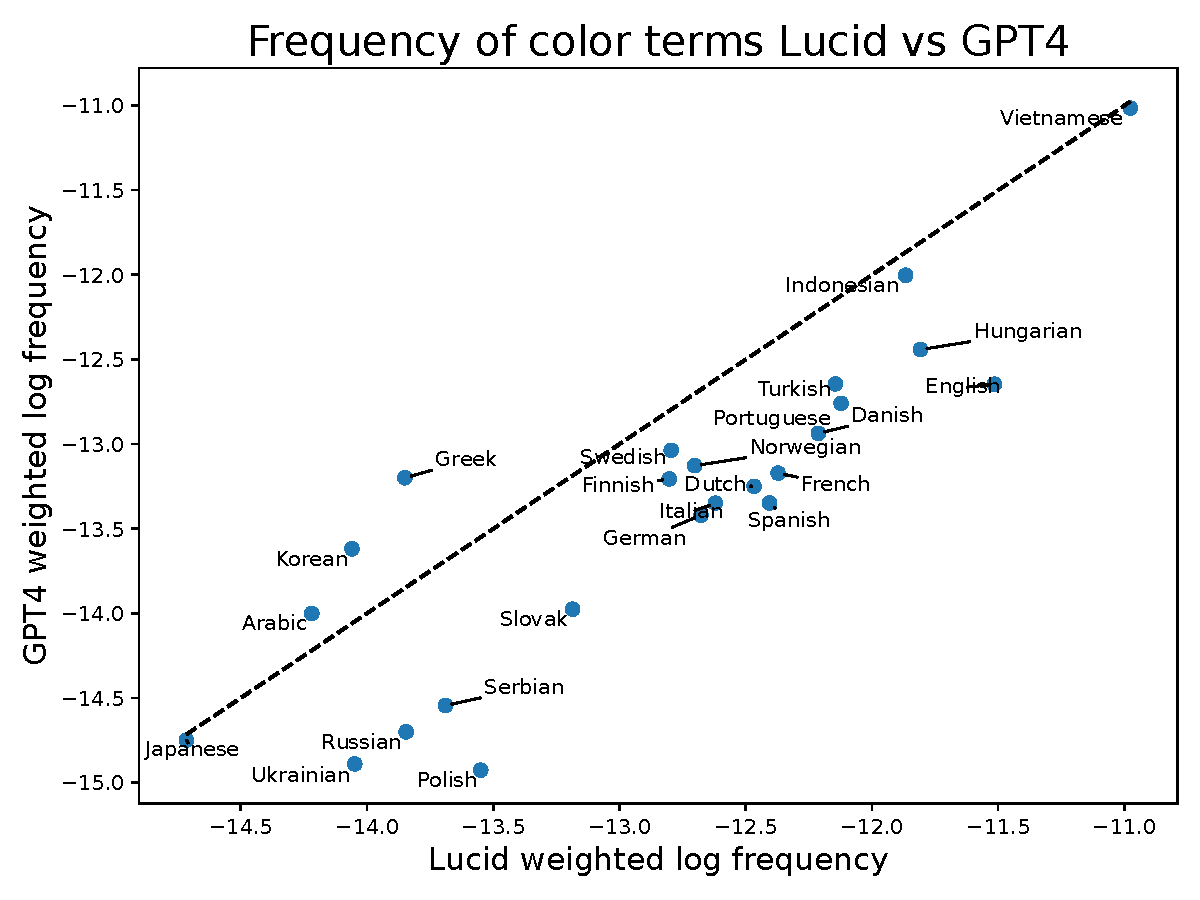
\includegraphics[page=1, width=\linewidth]{images/frequency_plot.pdf}
\decoRule
\caption[Frequency of Color terms]{Logarithmic mean frequency of color terms across languages comparing human data with GPT4 output. The data suggest that GPT4 uses color terms that are less commonly used in the respective languages.}
\label{fig:frequency_plot}
\end{figure}

A further examination of the list of color terms across human and GPT4 data showed a higher usage of infrequently used color terms in the respective languages for GPT4 (Fig. \ref{fig:frequency_plot}).
Apart from Arabic, Korean and Greek GPT4 employ overall less frequently used color terms. This might be related to the specific scripts they used. Compared to the other languages the cleaning heuristics apply fundamental changes in these cases such as the conversion into another script. This might case that the single terms might be less efficiently mapped to words in the respective language.
Whereas the distinction between GPT4 and human is almost significant (p=.059, via the Mann-Whitney U test) the relation is still highly correlated (r=.87, p<.000).


\begin{figure}[h!t]
\centering
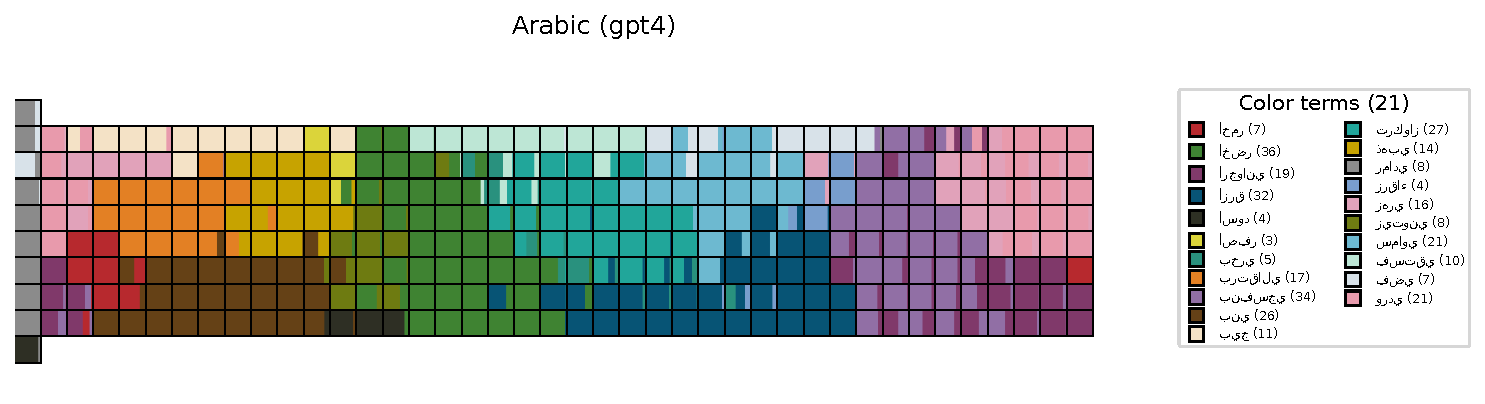
\includegraphics[width=0.49\linewidth]{images/mode_maps_gpt4/Arabic (gpt4).pdf}
\hfill
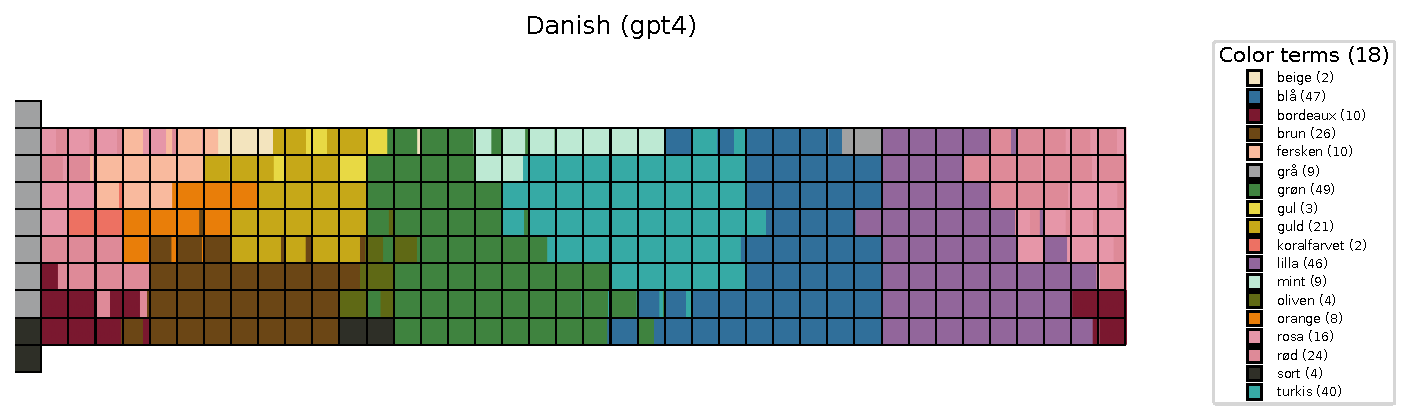
\includegraphics[width=0.49\linewidth]{images/mode_maps_gpt4/Danish (gpt4).pdf}
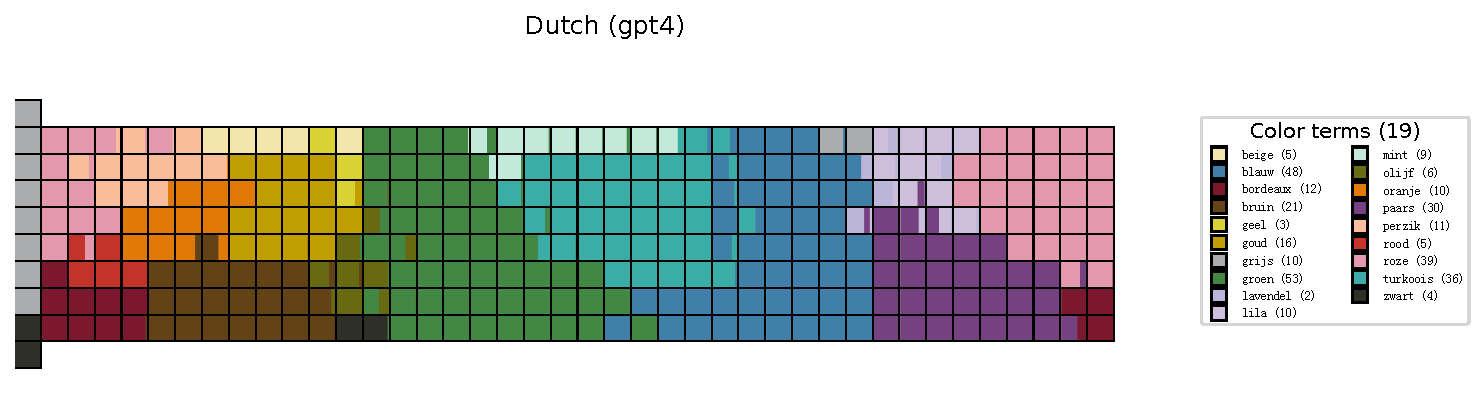
\includegraphics[width=0.49\linewidth]{images/mode_maps_gpt4/Dutch (gpt4).pdf}
\hfill
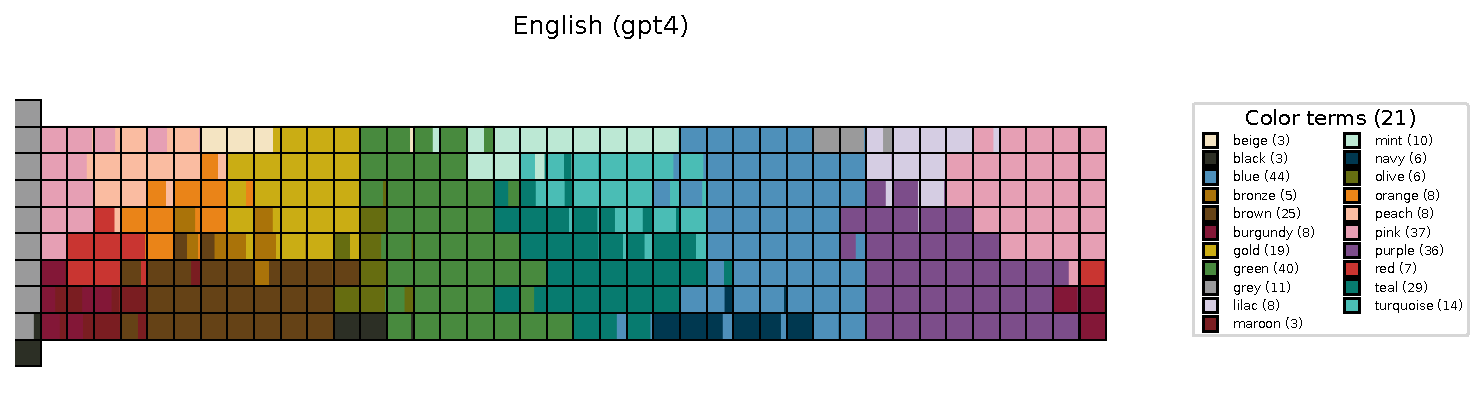
\includegraphics[width=0.49\linewidth]{images/mode_maps_gpt4/English (gpt4).pdf}
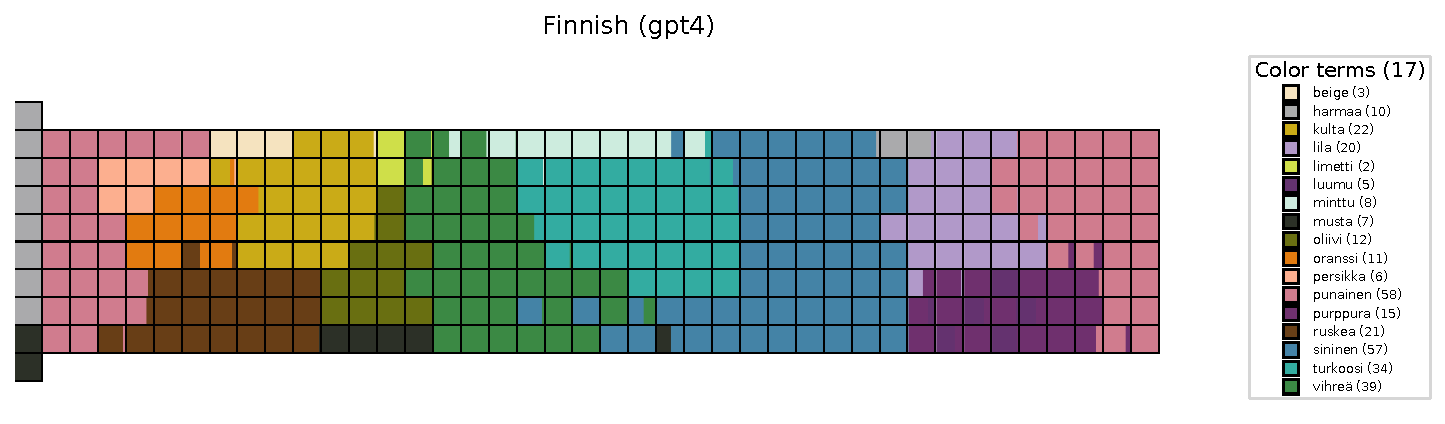
\includegraphics[width=0.49\linewidth]{images/mode_maps_gpt4/Finnish (gpt4).pdf}\hfill
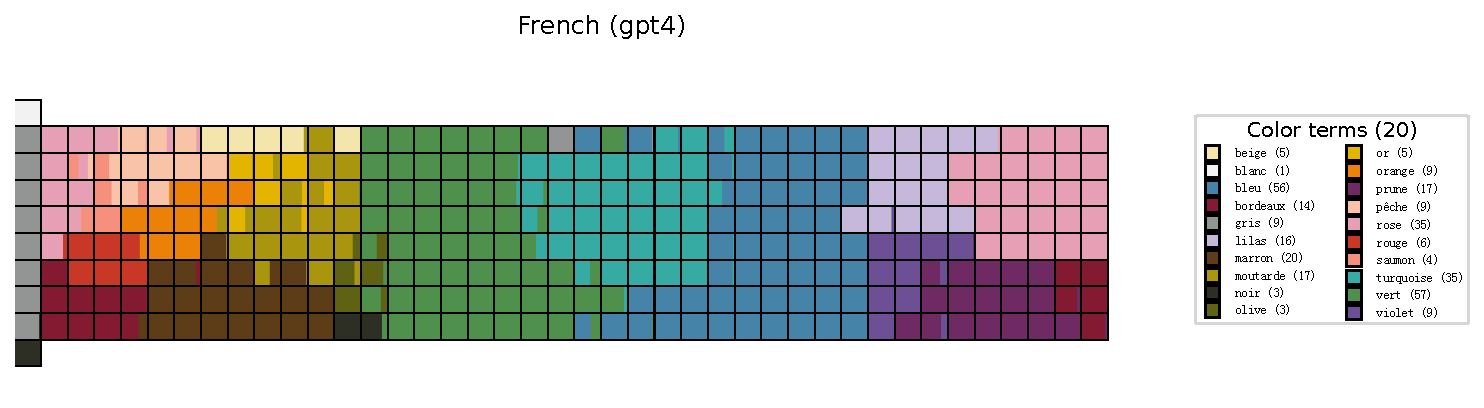
\includegraphics[width=0.49\linewidth]{images/mode_maps_gpt4/French (gpt4).pdf}
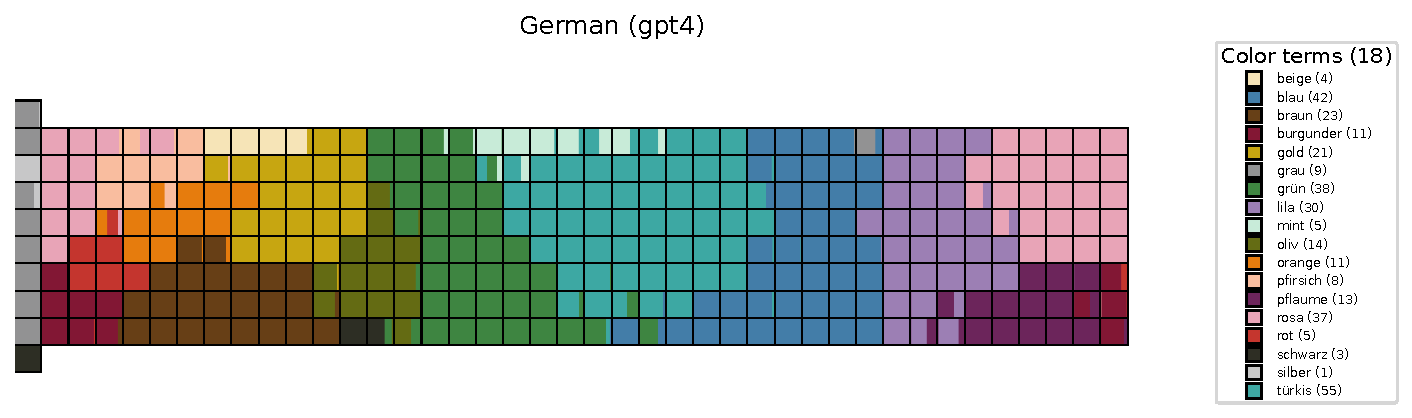
\includegraphics[width=0.49\linewidth]{images/mode_maps_gpt4/German (gpt4).pdf}\hfill
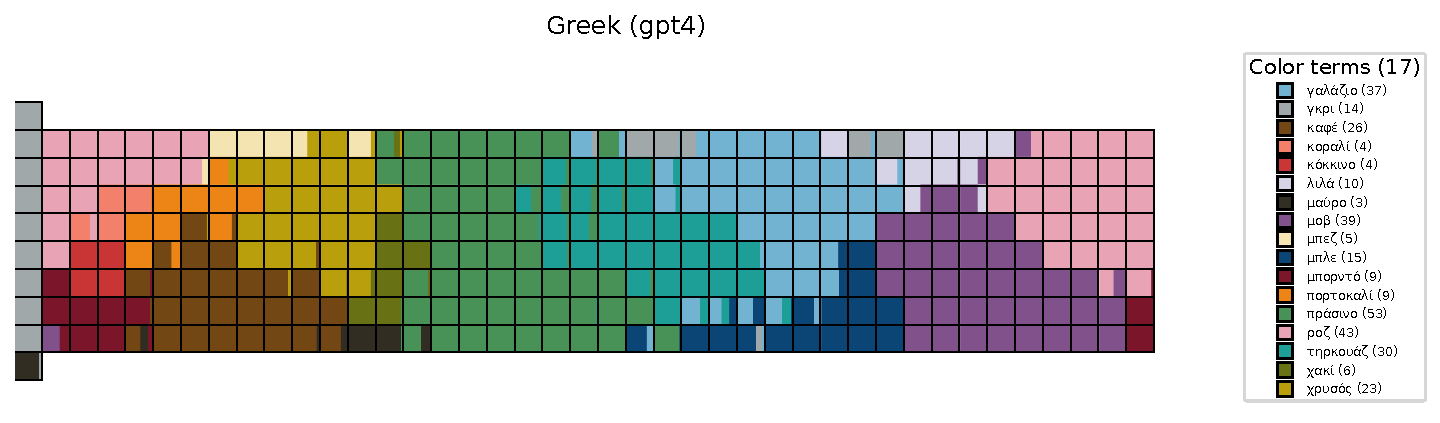
\includegraphics[width=0.49\linewidth]{images/mode_maps_gpt4/Greek (gpt4).pdf}
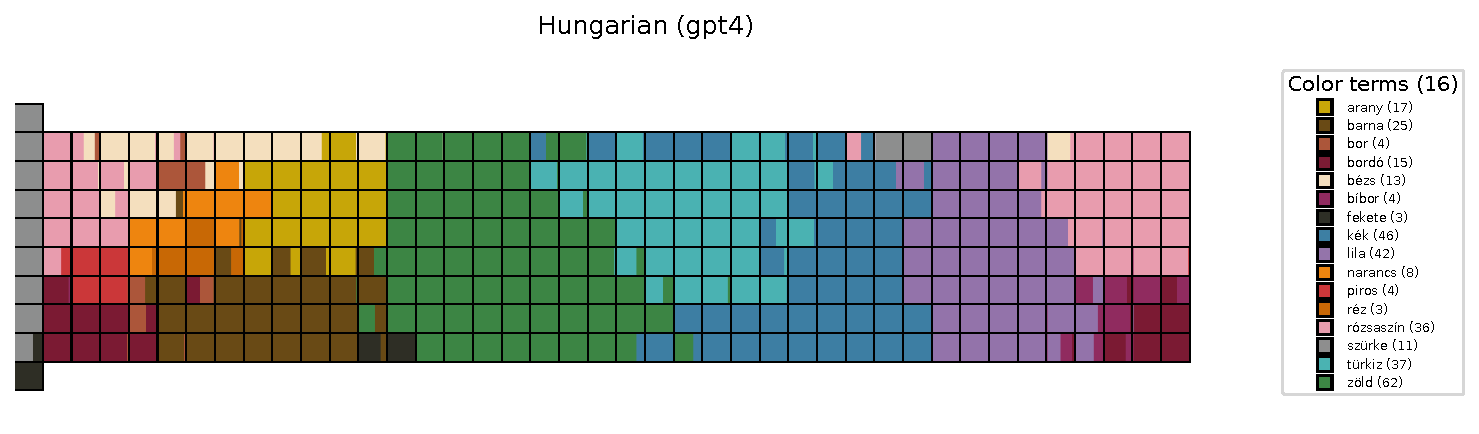
\includegraphics[width=0.49\linewidth]{images/mode_maps_gpt4/Hungarian (gpt4).pdf}
\hfill
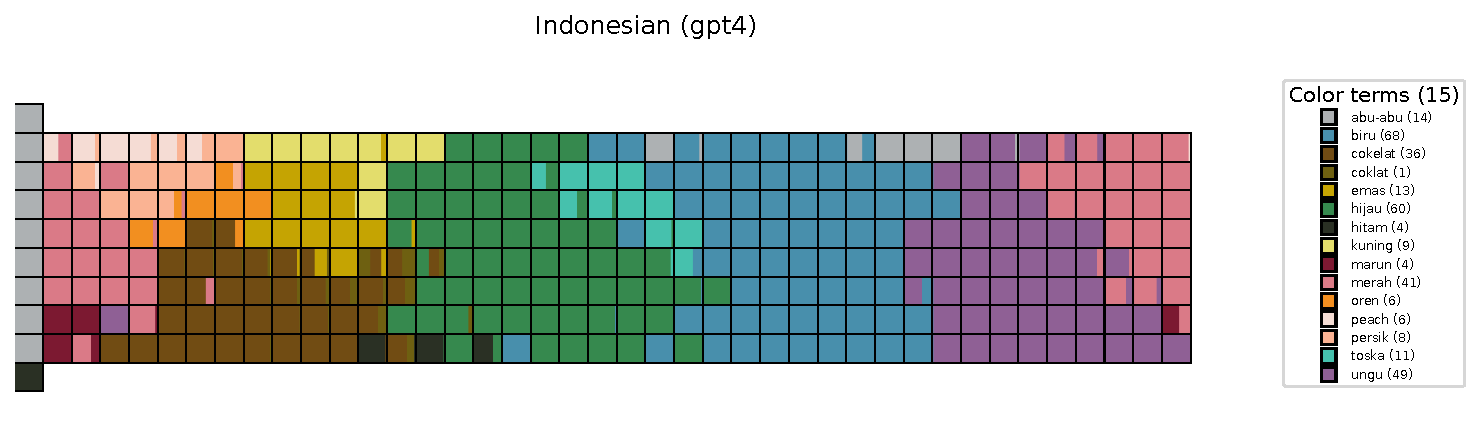
\includegraphics[width=0.49\linewidth]{images/mode_maps_gpt4/Indonesian (gpt4).pdf}
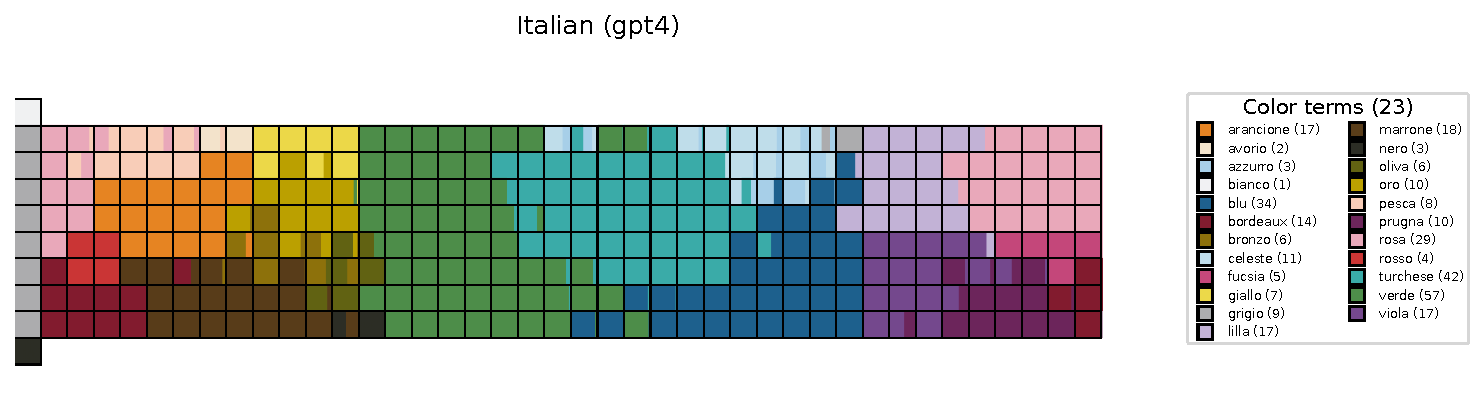
\includegraphics[width=0.49\linewidth]{images/mode_maps_gpt4/Italian (gpt4).pdf}
\hfill
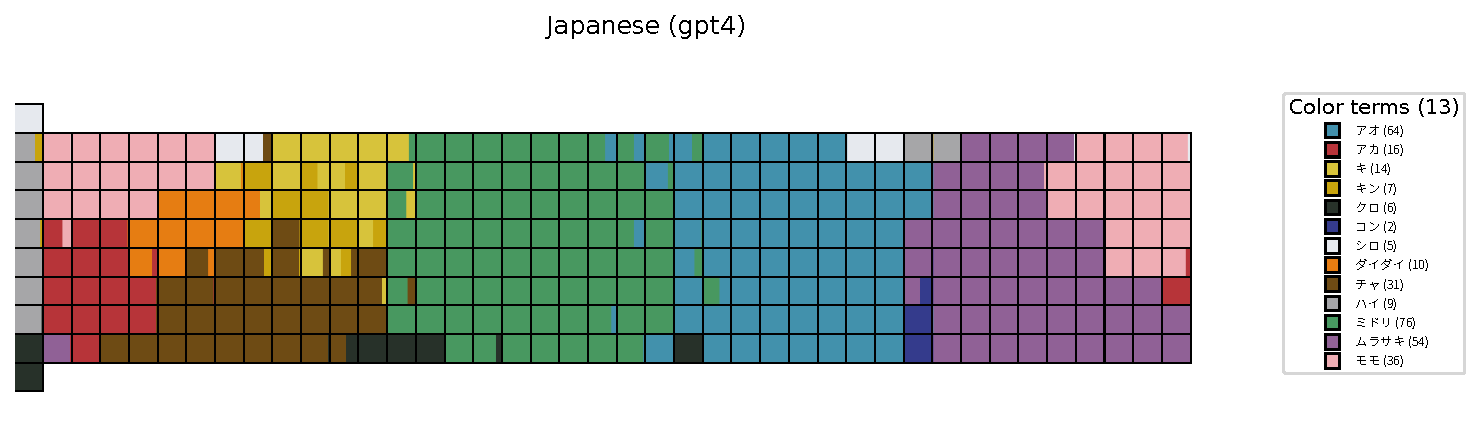
\includegraphics[width=0.49\linewidth]{images/mode_maps_gpt4/Japanese (gpt4).pdf}
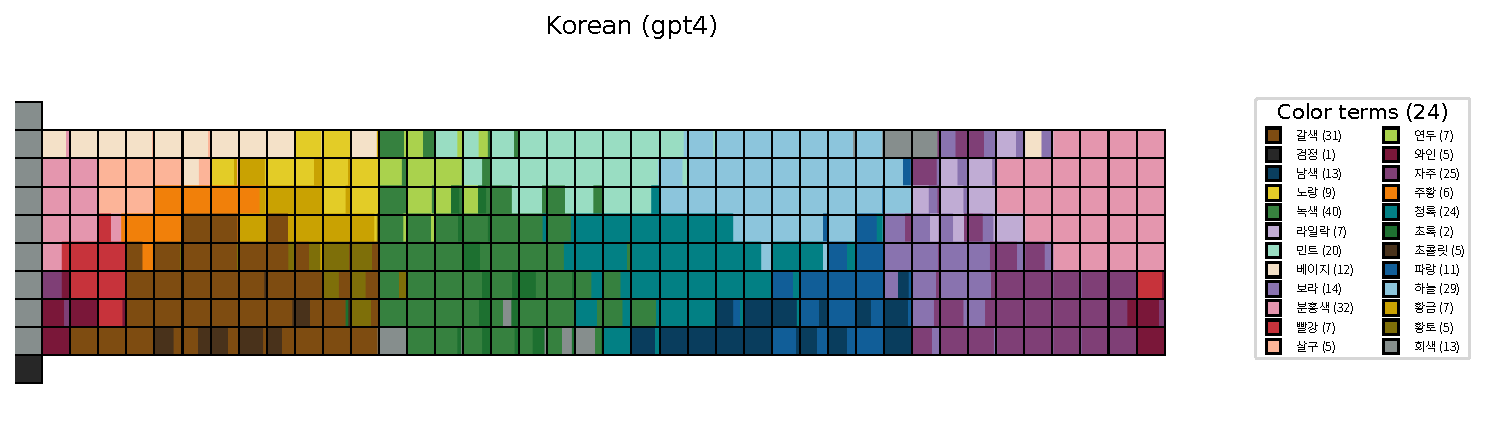
\includegraphics[width=0.49\linewidth]{images/mode_maps_gpt4/Korean (gpt4).pdf}
\hfill
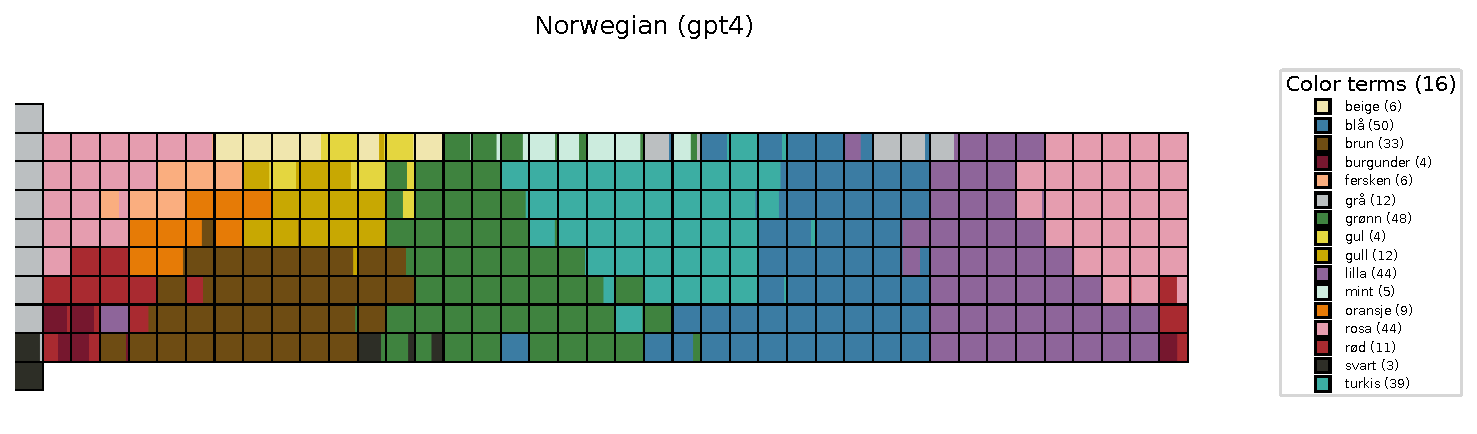
\includegraphics[width=0.49\linewidth]{images/mode_maps_gpt4/Norwegian (gpt4).pdf}
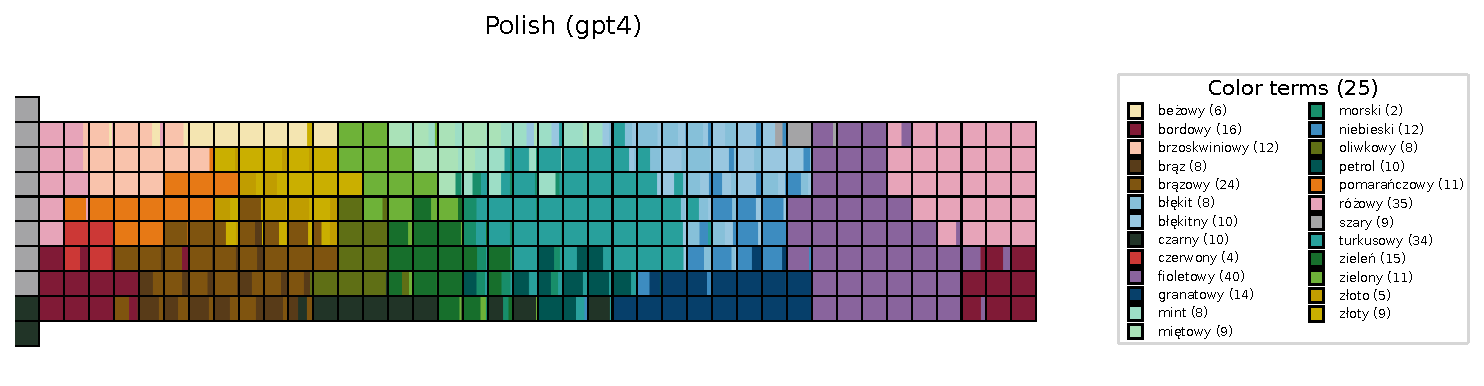
\includegraphics[width=0.49\linewidth]{images/mode_maps_gpt4/Polish (gpt4).pdf}
\hfill
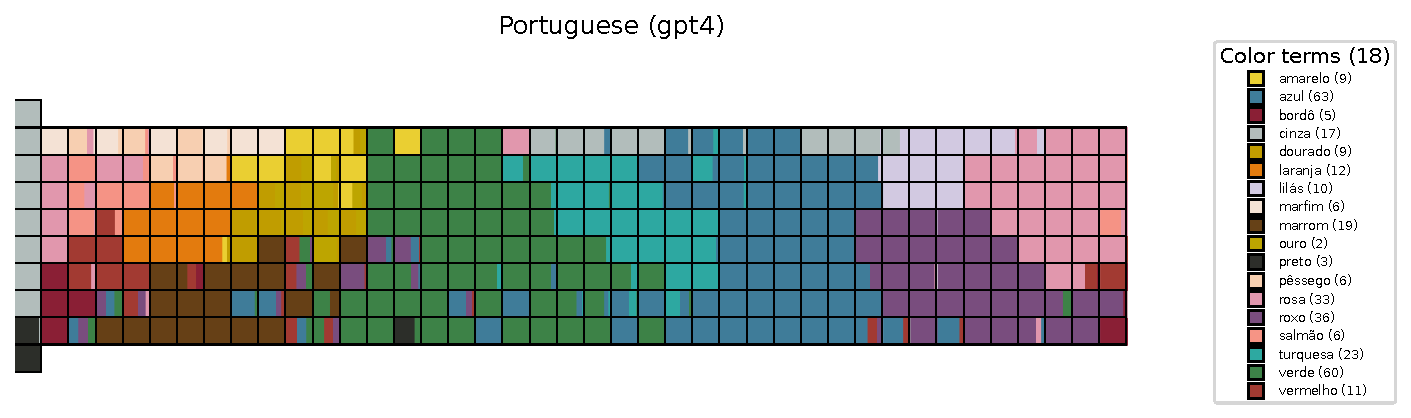
\includegraphics[width=0.49\linewidth]{images/mode_maps_gpt4/Portuguese (gpt4).pdf}
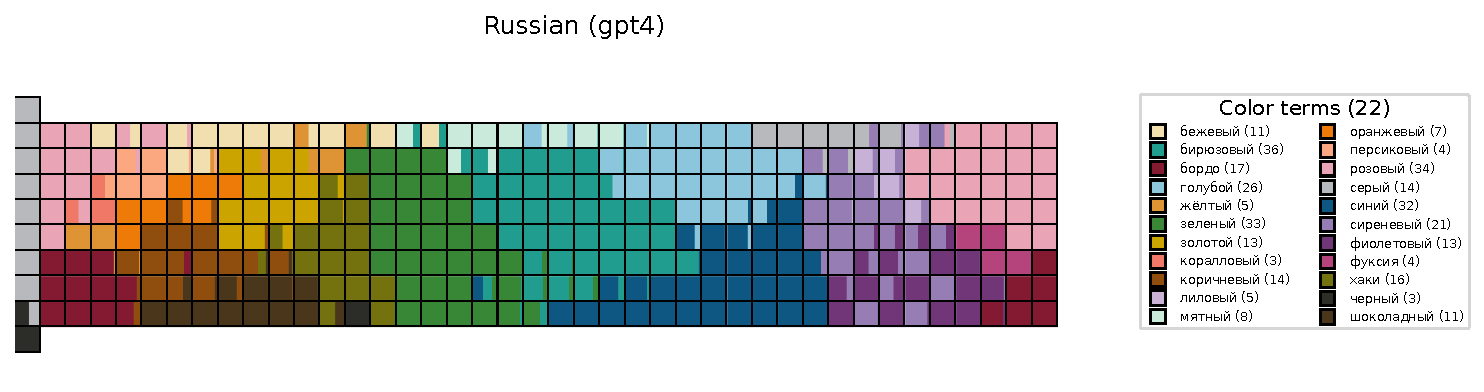
\includegraphics[width=0.49\linewidth]{images/mode_maps_gpt4/Russian (gpt4).pdf}
\hfill
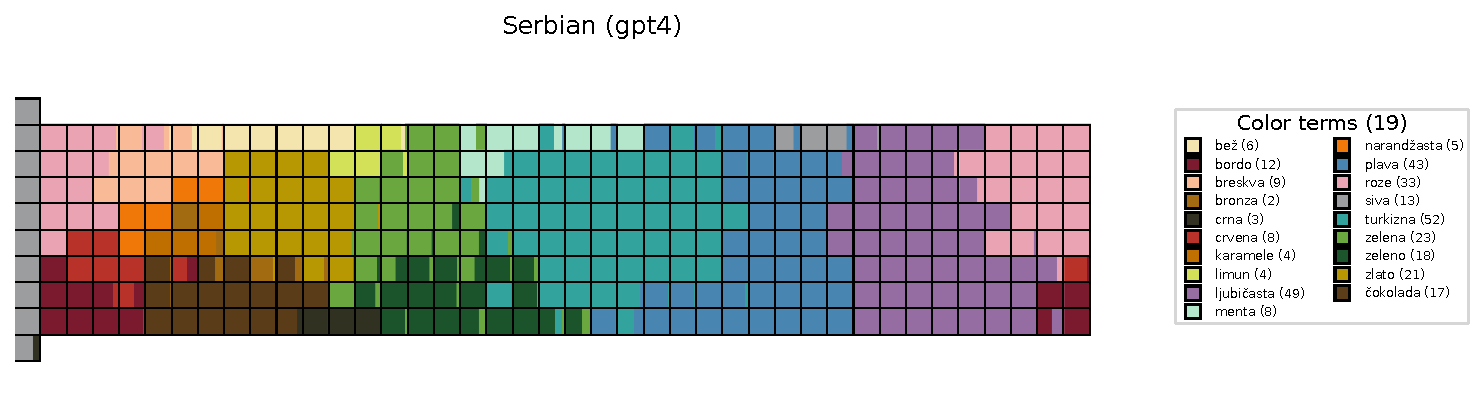
\includegraphics[width=0.49\linewidth]{images/mode_maps_gpt4/Serbian (gpt4).pdf}
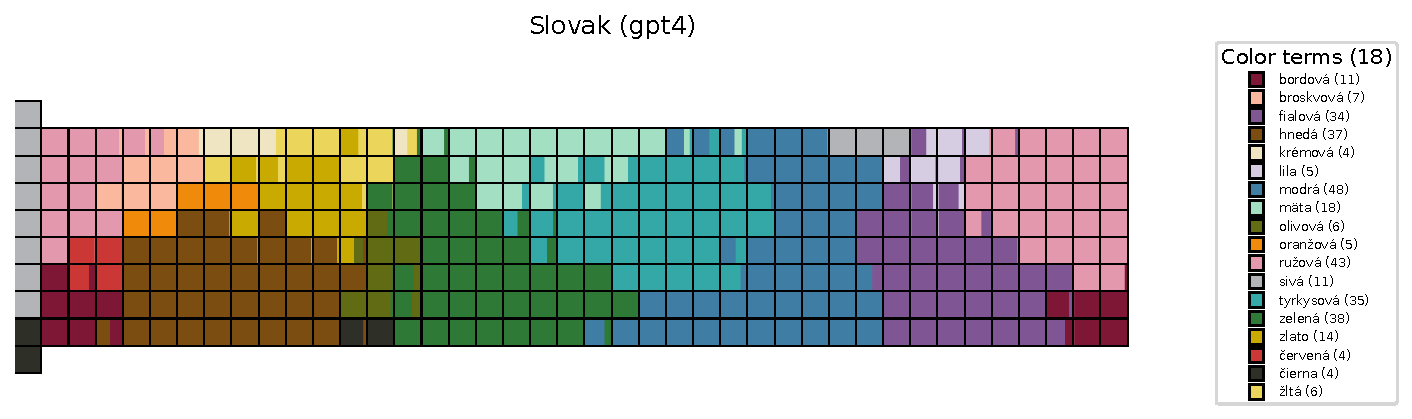
\includegraphics[width=0.49\linewidth]{images/mode_maps_gpt4/Slovak (gpt4).pdf}
\hfill
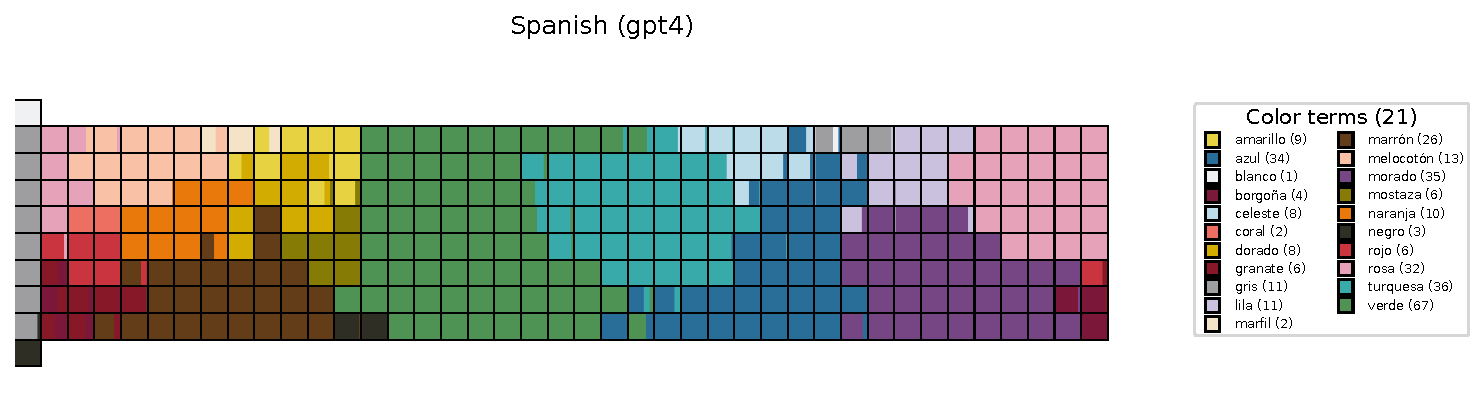
\includegraphics[width=0.49\linewidth]{images/mode_maps_gpt4/Spanish (gpt4).pdf}
\caption[GPT4 Proportion Plots]{GPT4 Proportion Plots}
\label{fig:mode-maps-gpt1}
\end{figure}


\begin{figure}[h!t]
\centering
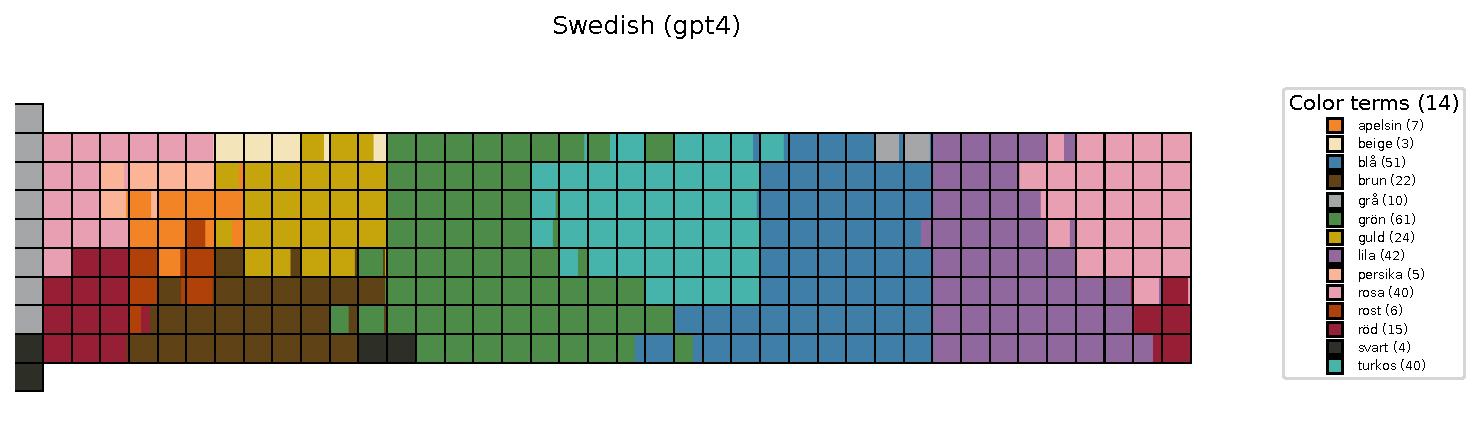
\includegraphics[width=0.49\linewidth]{images/mode_maps_gpt4/Swedish (gpt4).pdf}
\hfill
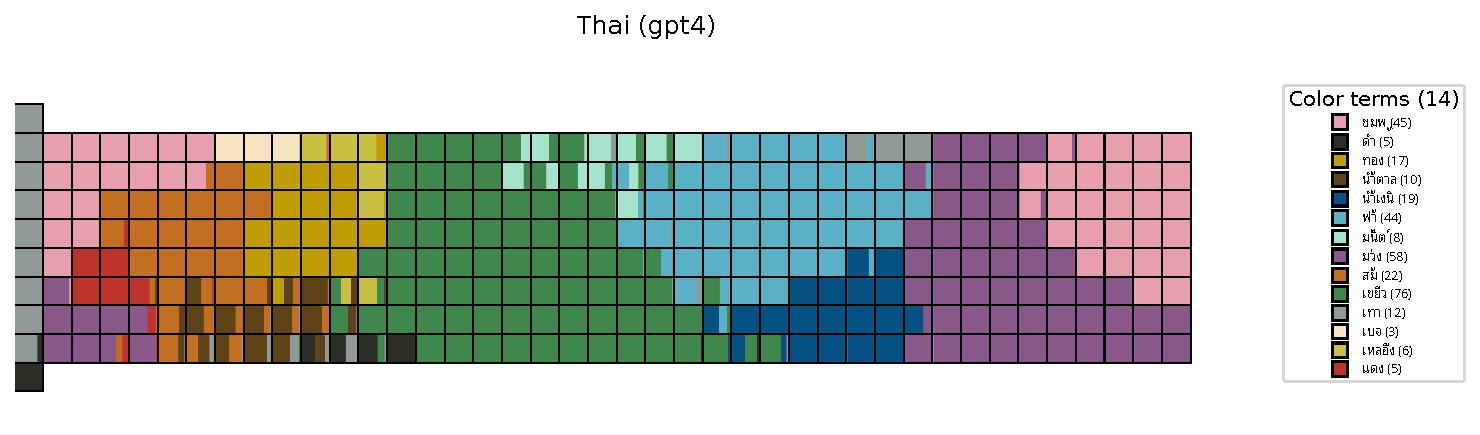
\includegraphics[width=0.49\linewidth]{images/mode_maps_gpt4/Thai (gpt4).pdf}
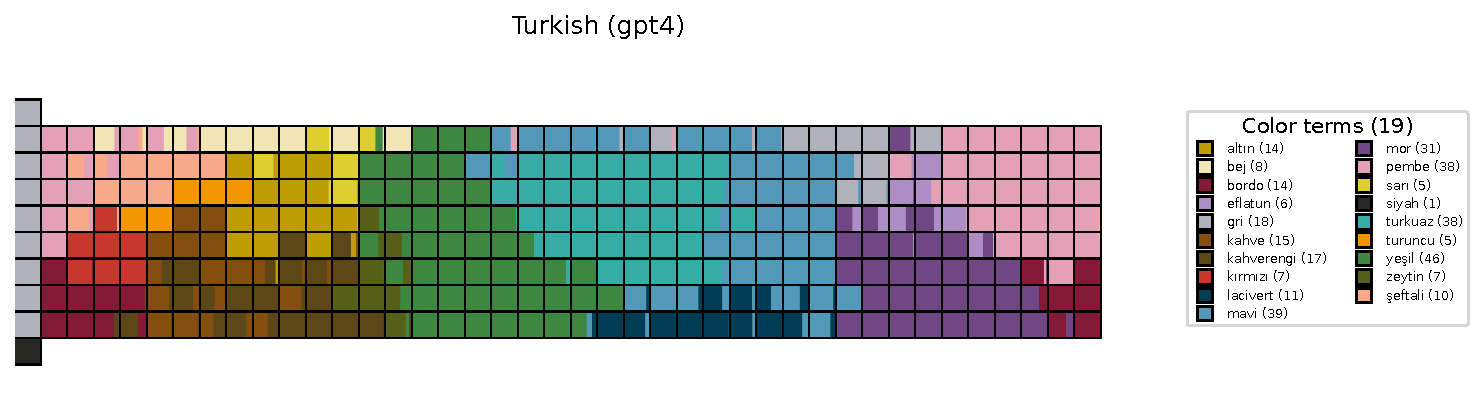
\includegraphics[width=0.49\linewidth]{images/mode_maps_gpt4/Turkish (gpt4).pdf}
\hfill
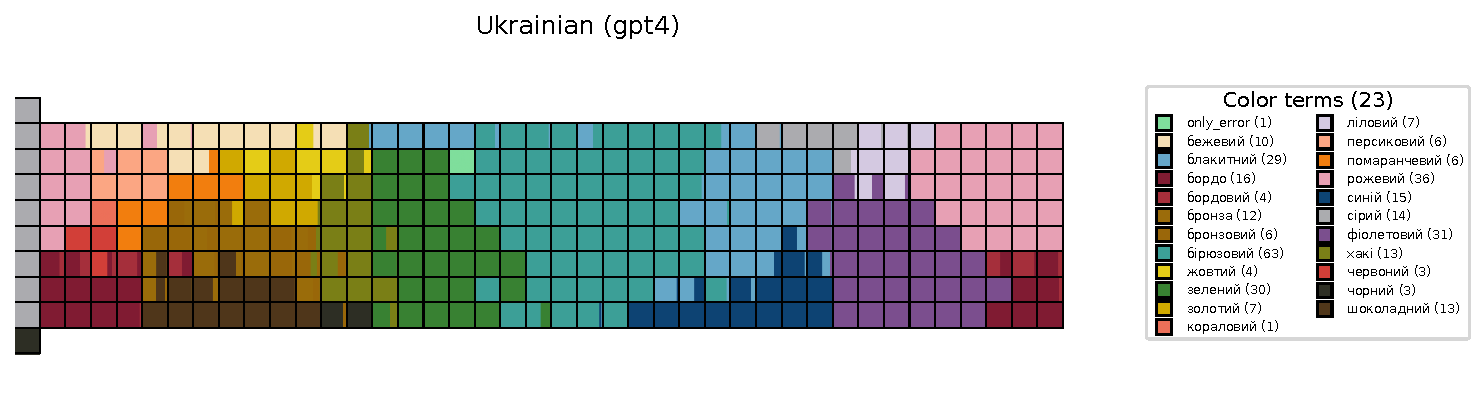
\includegraphics[width=0.49\linewidth]{images/mode_maps_gpt4/Ukrainian (gpt4).pdf}
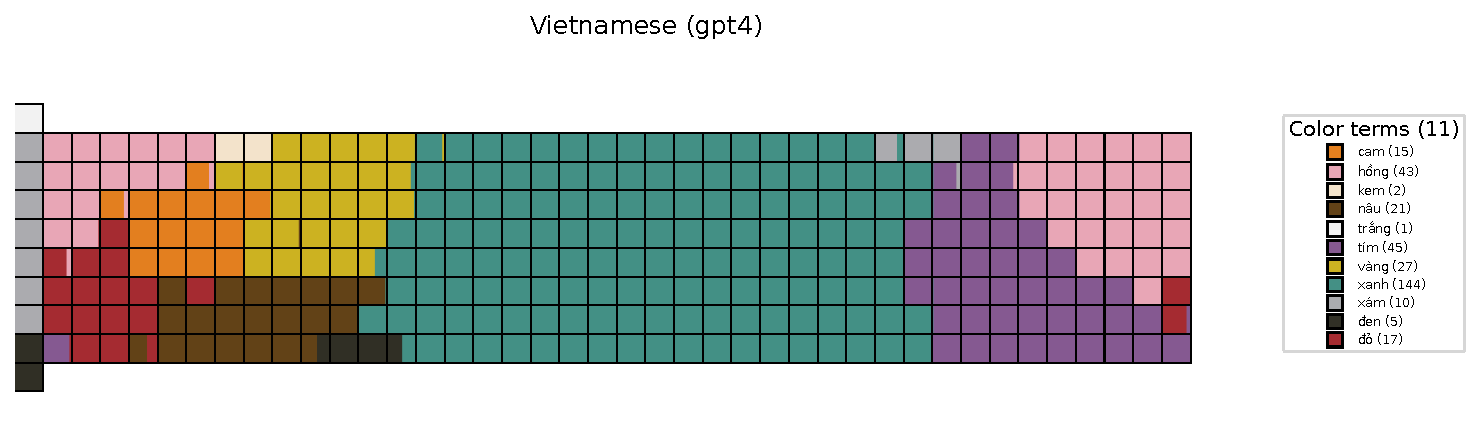
\includegraphics[width=0.49\linewidth]{images/mode_maps_gpt4/Vietnamese (gpt4).pdf}
\caption[GPT4 Proportion Plots]{GPT4 Proportion Plots}
\label{fig:mode-maps-gpt2}
\end{figure}


\chapter{Discussion}
Basis for the investigations of this project is the quality of the elicited data. Split half ARI was sufficiently high across the whole data set. Furthermore, a comparison with \textcite{lindseyColor2014}'s lab experiment and the data collected using Prolific as a traditional recruiter shows high ARI and therefore allows to relate the data sets to each other.

The Lucid data show higher overall ARI than the WCS dataset indicating a higher homogeneity across the languages. Newly examined languages use a higher number of color terms on average which is conform with the hypothesis of \textcite{berlinBasic1969} that languages develop new color terms when getting in touch with industrialized languages such as English.

In the single languages the white category was observed to be very small or absent which is due to the procedure of the experiment. The condition of the blue category was able to categorize most of the differences across languages. Using a MDS the languages were divided into a grue category, consisting solely of Vietnamese, the blue group of languages containing a large blue category and a light blue cluster with the blue category divided into a blue and a light blue category.

Investigations on the GPT4 data showed fundamental differences to the Lucid data. However, the relative positions of the languages within the batches are correlated for both GPT4 and GPT4-V. The comparison between individual languages showed a high overlap in the color terms used between GPT4 and Lucid data, even though GPT4 always used more specific color terms. Apparently, for many languages, GPT4 used loanwords from the English vocabulary to name niche colors like mint. This suggests a certain blurring of languages in GPT4's language production. The global and local entropy was then discovered to be responsible for much of the clustering in the MDS (Lucid-GPT4). For GPT4 and GPT4-V we saw very high global entropy reflecting what was stated above and low local entropy, which indicates a deterministic answering mechanism for GPT4. As expected, global entropy was higher in the Lucid dataset of industrialized languages, compared to the WCS languages, mostly unwritten languages. Local entropy was higher for the WCS but overlapped with the Lucid data. This means that the data sets are fundamentally different but still similar enough to form continuing and comparable data. Despite the differences, the number of color terms was correlated across GPT4 and Lucid data, meaning that languages of few color names in Lucid also had fewer color names in the GPT4 data. As mentioned above, GPT4 used more niche words for small categories. This was quantified by the average weighted log frequency which was lower for GPT4 data.


\section{Human Data}
Relative linguistics addresses the question whether language is shaped by thoughts or vice versa. To answer this question, much research has focused on the area of color terms because they have a direct physical correspondence. It was found that different languages use different numbers and constellations of color terms to subdivide color space. However, universal rules shaping these naming patterns were found and examined using, among others, the WCS dataset. \textcite{kayWorld2009} suspected that close cultural exchange between languages diminishes differences across languages as a globalization effect. Because of this in the WCS only languages spoken by small scale societies of limited cultural influence where examined. Industrialized countries were excluded from this data collection. They claimed to have found eleven BCT (equivalent to the English color names: \textit{black, white, red, yellow, green, blue, brown, orange, pink, purple, and gray}. They hypothesized that languages use these color categories or a subset of them. 

The collected data on lucid partially confirm these findings. For a large number of languages, labeled earlier as the blue cluster, we found high similarity to the English naming pattern and the number of major color categories. The grue category in Vietnamese also adapts to the evolutionary hypothesis that new categories emerge by partitioning of old categories. 

However, naming patterns of the languages previously grouped under the light blue cluster show major deviations. Most importantly, the additional universally present category \textit{light blue} shows a sophisticated division of the blue category. In Italian the blue category is even differentiated in three categories.
In addition, further diversification occurs such as \textgreek{λαδι} - oil as a major category between green and brown for Greek or \textkorean{연두색} for light green in Korean.
On the basis of these findings the limitation to the eleven BCT has to be rejected. Further, the preserved diversities across languages in spite of heavy exposure to cultural influence of internet users questions the hypothesized equalizing effect of globalization.
As expected, we were able to partly systematize the occurrence of additional color terms such as the light blue category in a high number of languages.
However, there were also other color categories emerging in single languages (e.g. \textgreek{λαδι} in greek) specific to the respective languages.

All measures of data quality such as split half ARI of single languages and comparisons between recruiters are sufficiently high and allow to contextualize our data to the literature. 
With minor exceptions the results for the single languages appear reasonable, ensuring the cleaning heuristics to work as expected.

Fig. \ref{fig:entropy_plot} highlights that the human data, both from WCS and from Lucid, form a continuum of growing number of color terms with the Lucid data located at the higher end, containing significantly more color terms. 
This confirms the hypothesis of \textcite{gibsonColor2017} that elevated contact to synthetic objects through industrialization drives the emergence and usage of more specific color terms. However, the mean ARI was significantly lower in all Lucid languages, indicating a more homogeneous data set overall. This in turn suggests a globalization effect in the industrialized languages. Finally, it should be noted that the cultural influence of globalization weakens diversity but does not completely eliminate it.



% The absence of the white category is most likely due to the way we present the stimulus \ref{fig:col-trail}. The square of color is presented on a white page. When showing very light chips a side effect might be that they never meet exactly the white of the page right next to the stimulus. The task undeliberately turn into a distinction task which makes it easy for people to see the very light color.



\section{Comparing Lucid - GPT4 Data}
The experiment was conducted in an analog manner using GPT4 and GPT4-V as agents. This was mainly done for two reasons. As LLMs evolve and enhance their capabilities, reliance on them by people intensifies. LLMs provide multifaceted assistance, assuming important roles and even supplanting jobs.
However, as LLMs are deep neural networks trained on large text corpora, we cannot be sure how exactly they work. Are they simulating human agents or behaving utterly different? At the same time LLMs can help to understand to what extend the perceptual environment can be recovered from language, which is a long standing problem in cognitive science.

As expected, we found correlation in the number of color terms for the same languages in GPT4 and Lucid data. Languages of smaller color term vocabularies in the human data tend to have fewer BCT named by GPT4. This result clearly supports the hypothesis that language specific naming patterns are conserved in the respective texts and subsequently reproduced by LLMs. Examining the behaviour of e.g. GPT4 then indeed can help to disentangle the relationship of language and its influence on perception.

However, we found fundamental differences between human and GPT4 data. The responding behaviour of GPT4 was much more deterministic on single chip level - almost robot-like, colloquially speaking. That means that GPT4 failed to mimic human-like behavior. Furthermore, GPT4 used much more niche color terms of lower usage frequency that did not occur in the Lucid data, indicating that GPT4 lacks common sense of what words should be used in an everyday conversation or what we referred to as BCT.

Considering GPT4 as a multilingual agent significantly influenced by globalization, the data indeed showed notable effects. For instance, English color terms like mint appeared in languages where mint is not a native word. This suggests that in some cases GPT4 mixes up words from different languages and imports them when the languages are missing terms for a particular hue.



% categories like mint imported from english


% Usage of infrequent color terms:
% GPT lacks common sense of which color terms are commonly used in an every day conversation.
\section{Limitations}

When asking participants to name colors, aiming to detect differences in these labeling patterns, it is key to actually present the exactly same colors. In e.g. the WCS and \textcite{lindseyColor2014} this was ensured by the use of the 330 physical Musell chips of high quality.
For this experiment this was not possible due to the fact that we use an online experiment approach. Therefore, we had to accommodate to the fact that every participant uses their own potentially calibrated screen to present the colors and then name it. In fact, different screen models, even with different calibration settings, display colors significantly differently \parencite{kwak2000characterisation}. As a consequence, this noise is included into our data, compared to the in-lab settings.
However, there are techniques to counteract this issue such as gamma correction. \textcite{xiao2011visual} invented a procedure to determine the current state of calibration of a screen based on the observers’ visual luminance judgements for the three channels red, green and blue. This is a very promising approach that was also implemented as a pre screen test for PsyNet. However, testing this procedure and establishing the scientific justification exceeded the time available for this master's thesis.

As mentioned in the introduction, online experiments also impose other limitations. The most basic criticism is the inability to maintain controlled environmental conditions, a standard rigorously upheld in laboratory-based experiments. It cannot be prevented that participants multitask at the same time. While this is certainly true, the collected data showed high similarity to the in-lab experiment conducted by \textcite{lindseyColor2014}. An option to further justify the results of this experiment would be to do a control experiment under lab conditions. Comparison between the remote procedure and the control experiment could then reveal the extend of influence of the online conditions have.

The sample of 25 languages is already a substantial set but does not include enough languages of the global South in particular, South America and Africa \parencite{barrett2020towards, blasi2022over}. Nonetheless, the innovative recruitment strategy has yielded reliable data, breaking ground for future data collection efforts in these regions. Looking forward we can potentially recruit even larger group of languages and cultures.

Ultimately, we believe this work paves the way for using diverse recruiting and machine learning to understand the human mind.
The results show high consistency across Lucid and the more traditional recruiter Prolific.
This lays the foundation for further leveraging Lucid's enormous recruiting potential.
For many languages we saw newly emerging color terms which can in part be condensed into major color categories such as light blue.
This indicates that the set of BCT is not ultimately restricted to eleven terms.
It is the duty of future research to monitor this development.
Furthermore, the preserved cross language differences within the GPT4 data has proven LLMs to be able to contribute to the science of color terms and thus to decipher the relation between thought and language.



\chapter{Code Availability} % Main appendix title
\label{code_availability} % Change X to a consecutive letter; for referencing this appendix elsewhere, use \ref{AppendixX}

The code for the psynet experiment is available here: \\
\url{https://gitlab.com/computational-audition-lab/wcs/color-naming-experiment}

The code used in order to clean, analyze and visualize data is available here: \\
\url{https://github.com/jakobpete/MasterThesisCode}


%\bibliographystyle{apacite}
\printbibliography[heading=bibintoc]

%\setlength{\bibleftmargin}{.125in}
%\setlength{\bibindent}{-\bibleftmargin}

%\listoffigures
%\bibliography{bibliography}
\end{document}
